\documentclass[12pt]{thesul}
%----------------------------------------------------------------------
%                               Packages
%----------------------------------------------------------------------
\usepackage[french]{babel}
\usepackage{acronym} % \ac[p], \acl[p], \acs[p], \acf[p]
\usepackage[sorting=none]{biblatex}
\bibliography{biblio.bib}
\usepackage{booktabs} % \toprule, \midrule, \cmidrule, \bottomrule
\usepackage{cancel} % \cancel
\usepackage{caption}
\usepackage{csquotes}
\usepackage{hyperref}
\hypersetup{hidelinks}
\usepackage[inline]{enumitem}
\setlist[enumerate]{label=(\roman*)} %% <- set the base level label separately
\usepackage{import} % \import
\usepackage[french]{minitoc}

\usepackage{xcolor}
\AtBeginDocument{
\definecolor{pdfurlcolor}{rgb}{0,0,0}
\definecolor{pdfcitecolor}{rgb}{0,0,0}
\definecolor{pdflinkcolor}{rgb}{0,0,0}
\definecolor{light}{gray}{.85}
\definecolor{vlight}{gray}{.95}
\definecolor{darkgreen}{RGB}{77,172,38}
\definecolor{darkblue}{RGB}{5,113,176}
\definecolor{mydarkblue}{RGB}{116,173,209}
\definecolor{mydarkblueid}{RGB}{83,154,198}
\definecolor{mylightblue}{RGB}{171,217,233}
\definecolor{mydarkorange}{RGB}{244,109,67}
\definecolor{mylightorange}{RGB}{252,153,54}
\definecolor{mydarkred}{RGB}{215,48,39}
\definecolor{mydarkpurple}{RGB}{140,107,177}
\definecolor{mydarkpurpleid}{RGB}{136,86,167}
}

\usepackage{amssymb}
\usepackage{amsmath}
\interdisplaylinepenalty=2500
\newtheorem{definition}{Définition}
\newtheorem{subdefinition}{Définition}[definition]
\newtheorem{myrule}{Règle}
\newtheorem{property}{Propriété}
\newtheorem{subproperty}{Propriété}[property]
\usepackage{MnSymbol} % \dashrightarrow

\usepackage{algorithm, algpseudocode}
\floatname{algorithm}{Algorithme} % Renomme caption de "Algorithm" -> "Algorithme"

\newcommand\CONDITION[2]%
  {\begin{tabular}[t]{@{}l@{}l@{}}
     #1&#2
   \end{tabular}%
  }
  \algdef{SE}[WHILE]{While}{EndWhile}[1]%
  {\algorithmicwhile\ \CONDITION{#1}{\ \algorithmicdo}}%
  {\algorithmicend\ \algorithmicwhile}
\algdef{SE}[FOR]{For}{EndFor}[1]%
  {\algorithmicfor\ \CONDITION{#1}{\ \algorithmicdo}}%
  {\algorithmicend\ \algorithmicfor}
\algdef{S}[FOR]{ForAll}[1]%
  {\algorithmicforall\ \CONDITION{#1}{\ \algorithmicdo}}
\algdef{SE}[REPEAT]{Repeat}{Until}{\algorithmicrepeat}[1]%
  {\algorithmicuntil\ \CONDITION{#1}{}}
\algdef{SE}[IF]{If}{EndIf}[1]%
  {\algorithmicif\ \CONDITION{#1}{\ \algorithmicthen}}%
  {\algorithmicend\ \algorithmicif}%
\algdef{C}[IF]{IF}{ElsIf}[1]%
  {\algorithmicelse\ \algorithmicif\ \CONDITION{#1}{\ \algorithmicthen}}

\usepackage[draft,inline,nomargin,index]{fixme}
\fxsetup{theme=color,mode=multiuser,inlineface=\itshape,envface=\itshape}
\FXRegisterAuthor{mn}{amn}{Matthieu}

\usepackage{tikz} % \begin{tikzpicture} \end{tikzpicture}
\usetikzlibrary{calc}
\usetikzlibrary{graphs}
\usetikzlibrary{quotes}
\usetikzlibrary{shapes.misc}

\usepackage[caption=false,font=footnotesize,labelfont=sf,textfont=sf]{subfig}

\usepackage{pifont} % \ding
\renewcommand{\checkmark}{\ding{51}}
\newcommand{\ballotx}{\ding{55}}

\usepackage{xspace} % \xspace

% Commands
%---------
\newcommand{\cf}[1]{(cf. \autoref{#1}, page \pageref{#1})}
\newcommand{\eg}{e.g.\xspace}
\newcommand{\ie}{c.-à-d.\xspace}

\newcommand{\hb}{\emph{happens-before}\xspace}

\newcommand{\inbb}[1]{\in \mathbb{#1}}
\newcommand{\new}{\textbf{new}}
\newcommand{\trm}[1]{\mathit{#1}}
\newcommand{\set}[1]{\left\{#1\right\}} % set brace notation

\newcommand{\betterid}[3]{\trm{#1}^{\trm{#2}}_{\trm{#3}}}
\newcommand{\id}[3]{$\trm{#1}^{\trm{#2}}_{\trm{#3}}$}
\newcommand{\epoch}[1]{$\varepsilon_{#1}$}
\newcommand{\lid}{<_{id}}
\newcommand{\leqid}{$\leq_{id}$~}
\newcommand{\lepoch}{$<_{\varepsilon}$~}
\newcommand{\leqepoch}{$\leq_{\varepsilon}$~}
\newcommand{\ltuple}{<_{t}}

\newcommand{\botn}{\bot_\mathbb{N}}
\newcommand{\topn}{\top_\mathbb{N}}
\newcommand{\logootuple}[1]{\langle \text{pos}_{#1},\text{nodeId}_{#1},\text{seq}_{#1} \rangle}

\newcommand{\bigO}[1]{$\mathcal{O}(#1)$}

\newcommand{\widthletter}{2em}
\newcommand{\widthblock}{3em}
\newcommand{\widthoriginepoch}{1.33em}
\newcommand{\widthepoch}{1.65em}

% Définit noms pour \autoref
%---------
\newcommand{\algorithmautorefname}{Algorithme}
\newcommand{\annexautorefname}{Annexe}
\newcommand{\definitionautorefname}{Définition}
\newcommand{\propertyautorefname}{Propriété}
\newcommand{\subfigureautorefname}{Figure}
\newcommand{\subpropertyautorefname}{Propriété}

% Tikz styles
\tikzset{
    common/.style={anchor=west, draw, rectangle, minimum height=6mm},
    letter/.style={common, minimum width=\widthletter},
    block/.style={common, minimum width=\widthblock},
    epoch/.style={letter, rounded rectangle, rounded rectangle east arc=0pt, minimum width=\widthepoch},
    point/.style={insert path={ node[scale=5*sqrt(\pgflinewidth)]{.} }},
    node/.style={draw, circle, minimum size=1em},
    op/.style={draw, circle, minimum size=2.7em},
    causalop/.style={op, double=white, inner sep=2pt},
    gc-rule-1/.style={dashed, thick, darkblue},
    gc-rule-2/.style={densely dotted, thick, darkgreen},
    cross/.style={
        path picture={
            \draw[mydarkred, very thick]
                (path picture bounding box.south east)--(path picture bounding box.north west)
                (path picture bounding box.south west)--(path picture bounding box.north east);
        }
    }
}


%-------------------------------------------------------------------
%                             Marges
%-------------------------------------------------------------------

% pour positionner les vraies marges:
%\SetRealMargins{1mm}{1mm}

%-------------------------------------------------------------------
%                             En-têtes
%-------------------------------------------------------------------

% Les en-têtes: quelques exemples
%\UppercaseHeadings
%\UnderlineHeadings
%\newcommand\bfheadings[1]{{\bf #1}}
%\FormatHeadingsWith{\bfheadings}
%\FormatHeadingsWith{\uppercase}
%\FormatHeadingsWith{\underline}
\newcommand\upun[1]{\uppercase{\underline{\underline{#1}}}}
\FormatHeadingsWith\upun

\newcommand\itheadings[1]{\textit{#1}}
\FormatHeadingsWith{\itheadings}

% pour avoir un trait sous l'en-tete:
\setlength{\HeadRuleWidth}{0.4pt}

%-------------------------------------------------------------------
%                         Les références
%-------------------------------------------------------------------

\NoChapterNumberInRef
\NoChapterPrefix

%-------------------------------------------------------------------
%                           Brouillons
%-------------------------------------------------------------------

% ceci ajoute une marque « brouillon » et la date
\ThesisDraft

%-------------------------------------------------------------------
%                   Pour collecter un glossaire et un index
%-------------------------------------------------------------------

\makeglossary
\makeindex

%-------------------------------------------------------------------
%                           Acronymes
%-------------------------------------------------------------------

% Acronyms
% --------
% \input{assets/acronyms.tex}
\acrodef{ADT}[ADT]{Abstract Data Type}
\acrodefplural{ADT}[ADTs]{Abstract Data Types}
\acrodef{API}[API]{Application Programming Interface}
\acrodef{AW}[AW]{\emph{Add-Wins}}
\acrodef{CCI}[CCI]{Convergence, Causality preservation, Intention preservation}
\acrodef{CL}[CL]{\emph{Causal-Length}}
\acrodef{CRDT}[CRDT]{Conflict-free Replicated Data Type}
\acrodefplural{CRDT}[CRDTs]{Conflict-free Replicated Data Types}
\acrodef{FIFO}[FIFO]{First In, First Out}
\acrodef{GC}[GC]{Garbage Collection}
\acrodef{JIT}[JIT]{Just-In-Time}
\acrodef{LCA}[PPAC]{Plus Petit Ancêtre Commun}
\acrodef{LUB}[LUB]{Least Upper Bound}
\acrodef{LWW}[LWW]{\emph{Last-Writer-Wins}}
\acrodef{MUTE}[MUTE]{Multi User Text Editor}
\acrodef{MV}[MV]{\emph{Multi-Value}}
\acrodef{OC}[OC]{Operation Commutativity}
\acrodef{OT}[OT]{Operational Transformation}
\acrodefplural{OT}[OT]{Operational Transformations}
\acrodef{P2P}[P2P]{Pair-à-Pair}
\acrodef{PKI}[PKI]{Public Key Infrastructure}
\acrodef{PT}[PT]{Precedence Transitivity}
\acrodef{RADT}[RADT]{Replicated Abstract Data Type}
\acrodefplural{RADT}[RADTs]{Replicated Abstract Data Types}
\acrodef{RGA}[RGA]{Replicated Growable Array}
\acrodef{RW}[RW]{\emph{Remove-Wins}}
\acrodef{SEC}[SEC]{Cohérence forte à terme}
\acrodef{TTF}[TTF]{Tombstone Transformation Function}
\acrodefplural{TTF}[TTF]{Tombstone Transformation Functions}
\acrodef{WebRTC}[WebRTC]{Web Real-Time Communication}

%-------------------------------------------------------------------
%                           Couleurs
%-------------------------------------------------------------------

% \input{assets/colours.tex}

%-------------------------------------------------------------------
%                     Global custom tikz commands
%-------------------------------------------------------------------

% \input{assets/tikz_presets.tex}

\begin{document}


      \OddHead={{\leftmark\rightmark}{\hfil\slshape\rightmark}}
      \EvenHead={{\leftmark}{{\slshape\leftmark}\hfil}}
      \OddFoot={\hfil\thepage}
      \EvenFoot={\thepage\hfil}
      \pagestyle{ThesisHeadingsII}


%-------------------------------------------------------------------
%                          Encadrements
%-------------------------------------------------------------------

% encadre les chapitres dans la table des matières:
% (ces commandes doivent figurer apres \begin{document}

\FrameChaptersInToc
%\FramePartsInToc


%-------------------------------------------------------------------
%            Réinitialisation de la numérotation des chapitres
%-------------------------------------------------------------------

% Si la commande suivante est présente,
% elle doit figurer APRÈS \begin{document}
% et avant la première commande \part
\ResetChaptersAtParts

%-------------------------------------------------------------------
%               mini-tables des matières par chapitre
%-------------------------------------------------------------------

% préparer les mini-tables des matières par chapitre.
% (commande de minitoc.sty)
\dominitoc

%-------------------------------------------------------------------
%                         Page de titre:
%-------------------------------------------------------------------

\ThesisTitle{Ré-identification sans coordination dans les types de données répliquées sans conflits (CRDTs)}
\ThesisDate{TODO: Définir une date}
\ThesisAuthor{Matthieu Nicolas}

% Type de la these
\ThesisUL
% Jury:

% (ne pas mettre de \\ apres la dernière entree)

% Exemple de création d'une nouvelle catégorie dans le jury:

\NewJuryCategory{family}{\it Membre de la famille :}
                        {\it Membres de la famille :}

\family={Mon frère\\Ma sœur}

\def\blanc{\hspace*{1cm}}

\President    = {Stephan Merz}
\Rapporteurs  = {Le rapporteur 1&de Paris\\
                 Le rapporteur 2\\
                 \blanc suite&taratata\\
                 Le rapporteur 3}
\Examinateurs = {L'examinateur 1&d'ici\\
                 L'examinateur 2}
%\Invites=       {}

% Création de la page de titre:
\MakeThesisTitlePage

%-------------------------------------------------------------------


%-------------------------------------------------------------------
%                          remerciements
%-------------------------------------------------------------------

%\DontFrameThisInToc
\begin{ThesisAcknowledgments}
WIP
\end{ThesisAcknowledgments}

%-------------------------------------------------------------------
%                            dédicace
%-------------------------------------------------------------------

\begin{ThesisDedication}
WIP
\end{ThesisDedication}


%-------------------------------------------------------------------
%                  écriture de `Chapitre' et `Partie'
%                      dans la table des matières
%-------------------------------------------------------------------

\WritePartLabelInToc
\WriteChapterLabelInToc

%-------------------------------------------------------------------
%                        table des matières
%-------------------------------------------------------------------

\tableofcontents

%-------------------------------------------------------------------
%              Exemple d'utilisation de \SpecialSection
%-------------------------------------------------------------------
%\SpecialSection{Introduction générale}

\DontWriteThisInToc
\listoffigures

\mainmatter
\NumberThisInToc
\chapter*{Introduction}
\minitoc
\section{Contexte}

\begin{itemize}
  \item Systèmes collaboratifs (wikis, plateformes de contenu, réseaux sociaux) et leurs bienfaits (qualité de l'info, vitesse de l'info (exemple de crise ?), diffusion de la parole).
    Démocratisation (sic) de ces systèmes au cours de la dernière décennie.
  \item En raison du volume de données et de requêtes, adoptent architecture décentralisée.
    Permet ainsi de garantir disponibilité, tolérance aux pannes et capacité de passage à l'échelle.
  \item Mais échoue à adresser problèmes non-techniques : confidentialité, souveraineté, protection contre censure, dépendance et nécessité de confiance envers autorité centrale.
  \item À l'heure où les entreprises derrière ces systèmes font preuve d'ingérence et d'intérêts contraires à ceux de leurs utilisateur-rices (Cambridge Analytica, Prism, non-modération/mise en avant de contenus racistes \footnote{\emph{Algorithms of Oppression}, Safiya Umoja Noble}\footnote{\url{https://www.researchgate.net/publication/342113147_The_YouTube_Algorithm_and_the_Alt-Right_Filter_Bubble}}\footnote{\url{https://www.wsj.com/articles/the-facebook-files-11631713039}}, invisibilisation de contenus féministes, dissolution du comité d'éthique de Google\footnote{\url{https://www.bbc.com/news/technology-56135817}}, inégalité d'accès à la méta-machine affectante\footnote{\emph{Je suis une fille sans histoire}, Alice Zeniter, p. 75}\footnote{Qui cite \emph{Les affects de la politique}, Frédéric Lordon}\footnote{\url{https://www.bbc.com/news/technology-59011271}}), parait fondamental de proposer les moyens technologiques accessibles pour concevoir et déployer des alternatives.
  \item \mnnote{TODO: Voir si angle écologique/réduction consommation d'énergie peut être pertinent.}
  \item Systèmes pair-à-pair sont une direction intéressante pour répondre à ces problématiques, de part leur absence d'autorité centrale, la distribution des tâches et leur conception mettant le pair au centre.
    Mais posent de nouvelles problématiques de recherche.
  \item Ces systèmes ne disposent d'aucun contrôle sur les noeuds qui les composent.
    Le nombre de noeuds peut donc croître de manière non-bornée et atteindre des centaines de milliers de noeuds.
    La complexité des algorithmes de ces systèmes ne doit donc pas dépendre de ce paramètre, ou alors de manière logarithmique.
  \item De plus, ces noeuds n'offrent aucune garantie sur leur stabilité.
    Ils peuvent donc rejoindre et participer au système de manière éphèmère.
    S'agit du phénomène connu sous le nom de churn.
    Les algorithmes de ces systèmes ne peuvent donc pas reposer sur des mécanismes nécessitant une coordination synchrone d'une proportion des noeuds.
  \item Finalement, ces noeuds n'offrent aucune garanties sur leur fiabilité et intentions.
    Les noeuds peuvent se comporter de manière byzantine.
    Pour assurer la confidentialité, l'absence de confiance requise et le bon fonctionnement du système, ce dernier doit être conçu pour résister aux comportements byzantins de ses acteurs.
  \item Ainsi, il est nécessaire de faire progresser les technologies existantes pour les rendre compatible avec ce nouveau modèle de système.
    Dans le cadre de cette thèse, nous nous intéressons aux mécanismes de réplication de données dans les systèmes collaboratifs pair-à-pair temps réel.
\end{itemize}

\section{Questions de recherche et contributions}

\subsection{Ré-identification sans coordination pour \acp{CRDT} pour Séquence}

\begin{itemize}
  \item Systèmes collaboratifs permettent aux utilisateur-rices de manipuler et éditer un contenu partagé.
    Pour des raisons de performance, ces systèmes autorisent généralement les utilisateur-rices à effectuer des modifications sans coordination.
    Leur copies divergent alors momentanément.
    Un mécanisme de synchronisation leur permet ensuite de récupérer l'ensemble des modifications et de les intégrer, de façon à converger.
    Cependant, des modifications peuvent être incompatibles entre elles, car de sémantiques contraires.
    Un mécanisme de résolution de conflits est alors nécessaire.
  \item Les \acp{CRDT} sont des types de données répliquées.
    Ils sont conçus pour être répliqués par les noeuds d'un système et pour permettre à ces derniers de modifier les données partagées sans aucune coordination.
    Dans ce but, ils incluent des mécanismes de résolution de conflits directement au sein leur spécification.
    Ces mécanismes leur permettent de résoudre le problème évoqué précédemment.
    Cependant, ces mécanimes induisent un surcoût, aussi bien d'un point de vue consommation mémoire et réseau que computationnel.
    Notamment, certains \acp{CRDT} comme ceux pour la Séquence souffrent d'une croissance monotone de leur surcoût.
    Ce surcoût s'avère handicapant dans le contexte des collaborations à large échelle.
  \item Pouvons-nous proposer un mécanisme sans coordination de réduction du surcoût des \acp{CRDT} pour Séquence, \ie compatible avec les systèmes pair-à-pair ?
  \item Dans le cadre des \acp{CRDT} pour Séquence, le surcoût du type de données répliquées provient de la croissance de leurs métadonnées.
    Métadonnées proviennent des identifiants associés aux éléments de la Séquence par les \acp{CRDT}.
    Ces identifiants sont nécessaires pour le bon fonctionnement de leur mécanisme de résolution de conflits.
  \item Plusieurs approches ont été proposées pour réduire le coût de ces identifiants.
    Notamment, \cite{letia:hal-01248270,zawirski:hal-01248197} proposent un mécanisme de ré-assignation d'identifiants de façon à réduire leur taille.
    Mécanisme non commutatif avec les modifications concurrentes de la Séquence, \ie l'insertion ou la suppression.
    Propose ainsi un mécanisme de transformation des modifications concurrentes pour gérer ces conflits.
    Mais mécanisme de ré-assignation n'est pas non plus commutatif avec lui-même.
    De fait, utilisent un algorithme de consensus pour empêcher l'exécution du mécanisme en concurrence.
  \item Proposons RenamableLogootSplit, un nouveau \ac{CRDT} pour Séquence.
    Intègre un mécanisme de renommage directement au sein de sa spécification.
    Intègre un mécanisme de résolution de conflits pour les renommages concurrents.
    Permet ainsi l'utilisation du mécanisme de renommage par les noeuds sans coordination.
\end{itemize}

\subsection{Éditeur de texte collaboratif pair-à-pair}

\begin{itemize}
  \item Systèmes collaboratifs adoptent généralement architecture décentralisée.
    Disposent d'autorités centrales qui facilitent la collaboration, l'authentification des utilisateur-rices, la communication et le stockage des données.
  \item Mais ces systèmes introduisent une dépendance des utilisateur-rices envers ces mêmes autorités centrales, une perte de confidentialité et de souveraineté.
  \item Pouvons-nous concevoir un éditeur de texte collaboratif sans autorités centrales, \ie un éditeur de texte collaboratif à large échelle pair-à-pair ?
  \item Ce changement de modèle, d'une architecture décentralisée à une architecture pair-à-pair, introduit un ensemble de problématiques de domaines variés, \eg
    \begin{enumerate}
      \item Comment permettre aux utilisateur-rices de collaborer en l'absence d'autorités centrales pour résoudre les conflits de modifications ?
      \item Comment authentifier les utilisateur-rices en l'absence d'autorités centrales ?
      \item Comment structurer le réseau de manière efficace, \ie en limitant le nombre de connexion par pair ?
    \end{enumerate}
  \item Présentons \ac{MUTE} \cite{MUTE2017}.
    S'agit, à notre connaissance, du seul prototype complet d'éditeur de texte collaboratif temps réel pair-à-pair chiffré de bout en bout.
    Allie ainsi les résultats issus des travaux de l'équipe sur les \acp{CRDT} pour Séquence \cite{2013-logootsplit,2021-these-vic} et l'authentification des pairs dans systèmes distribués \cite{2018-trusternity-short,2018-trusternity-long} aux résultats de la littérature sur mécanismes de conscience de groupe \mnnote{TODO: Trouver et ajouter références}, les protocoles d'appartenance aux groupe \cite{swim2002, lifeguard2018}, les réseaux pair-à-pair \cite{2018-spray-nedelec} et les protocoles d'établissement de clés de groupe \cite{1995-burmester-desmedt}.
\end{itemize}

\section{Plan du manuscrit}
\section{Publications}

\NumberThisInToc
\chapter{État de l'art}
\minitoc

\section{Modèle du système}

\section{Systèmes distribués}
\section{Systèmes distribués}

\begin{itemize}
  \item Contexte des systèmes distribués à large échelle
  \item Réplique les données afin de pouvoir supporter les pannes
  \item Adopte le paradigme de la réplication optimiste \cite{10.1145/1057977.1057980}
  \item Autorise les noeuds à consulter et à modifier la donnée sans aucune coordination entre eux
  \item Autorise alors les noeuds à diverger temporairement
  \item Permet d'être toujours disponible, de toujours répondre aux requêtes même en cas de partition réseau
  \item Permet aussi, en temps normal, de réduire le temps de réponse (privilégie la latence) \cite{pacelc2012}
  \item Comme ce modèle autorise les noeuds à modifier la donnée sans se coordonner, possible d'effectuer des modifications concurrentes
  \item Généralement, un mécanisme de résolution de conflits est nécessaire afin d'assurer la convergence des noeuds dans une telle situation
  \item Plusieurs approches ont été proposées pour implémenter un tel mécanisme
\end{itemize}


% \section{Transformées opérationnelles}
% \begin{itemize}
  \item Approche permettant de gérer des modifications concurrentes sur un type de données
  \item Consiste à transformer les opérations par rapport aux effets des opérations concurrentes pour rendre les rendre commutatives.
    Permet de rendre l'ordre d'intégration des opérations sans importance par rapport à l'état final obtenu
  \item Se décompose en 2 parties : algorithmes (génériques) et fonctions de transformations (spécifiques au type de données)
  \item Plusieurs algorithmes OT adoptent une architecture centralisée (trouver citations)
  \item Cette architecture pose des problèmes de performances (bottleneck), sécurité (SPOF), coût, d'utilisabilité (mode offline), pérennité (disparition du service), vie privée et de résistance à la censure.
  \item Pour ces raisons, des algorithmes reposant sur une architecture décentralisée ont été proposés
  \item Mais ne règlent qu'en partie ces limites
  \item Notamment, ne sont pas adaptés à des systèmes P2P dynamiques
  \item Besoin de vector clocks sur chaque opération pour détecter la concurrence.
    Vector clocks adaptés dans systèmes à nombre de pairs fixe, mais pas aux systèmes dynamiques (revoir causal barrier pour p-e nuancer ce propos).
  \item Néanmoins, cette approche a permis de démocratiser les systèmes collaboratifs via son adoption par des services tels que Google Docs, Overleaf, Framapad
  \item De plus, dans le cadre de ces travaux, ont été définies les propriétés CCI \cite{10.1145/274444.274447}.
  \item Remettre en question la propriété Causalité des CCI.
    Généralement, confond causalité et happen-before et exprime en finalité une contrainte trop forte.
    Cette contrainte peut réduire la réactivité du système (exemple avec 2 insertions sans liens mais qui force d'attendre la 1ère pour intégrer la 2nde).
    Causalité pose aussi des problèmes de passage à l'échelle car repose sur vector clocks.
    IMO, doit relaxer cette propriété pour pouvoir construire systèmes à large échelle.
\end{itemize}

\mnnote{TODO: Mentionner TP1 et TP2}

\mnnote{TODO: Spécification faible et forte des séquences répliquées}


\section{Types de données répliquées sans conflits}
Pour limiter la coordination entre les noeuds, les systèmes distribués adoptent le paradigme de la réplication optimiste \cite{2005-optimistic-replication-saito}.
Ce paradigme consiste à ce que chaque noeud possède une copie de la donnée.
Chaque noeud possède le droit de la modifier sans se coordonner avec les autres noeuds.
Les noeuds peuvent alors temporairement diverger, \ie posséder des états différents.
Un mécanisme de synchronisation leur permet ensuite de partager leurs modifications respectives et de nouveau converger.
Ce paradigme offre ainsi aux noeuds une haute disponibilité \cite{2016-trade-offs-replicated-systems-guerraoui} ainsi qu'une faible latence.

Afin d'ordonner les évènements se produisant dans un système, la littérature repose généralement sur la relation \hb \cite{1978-happen-before-lamport}.
Nous l'adaptons ci-dessous à notre contexte :

\begin{definition}[Relation \hb]
  La relation \hb indique qu'une modification $m_1$ a eu lieu avant une modification $m_2$, notée $m_1 \rightarrow m_2$, si et seulement si une des conditions suivantes est satisfaite :
  \begin{enumerate}
    \item $m_1$ a eu lieu avant $m_2$ sur le même noeud.
    \item $m_1$ a été livrée au noeud auteur de $m_2$ avant la génération de $m_2$.
    \item Il existe une modification $m$ telle que $m_1 \rightarrow m \land m \rightarrow m_2$.
  \end{enumerate}
\end{definition}

Dans le cadre d'un système distribué, nous notons que la relation \hb ne permet pas d'établir un ordre total entre les modifications\footnote{Nous utilisons le terme \emph{modifications} pour désigner les \emph{opérations de modifications} des types abstraits de données afin d'éviter une confusion avec le terme \emph{opération} introduit ultérieurement.}.
En effet, deux modifications $m_1$ et $m_2$ peuvent être effectuées en parallèle par deux noeuds différents, sans avoir connaissance de la modification de leur pair respectif.
De telles modifications sont alors dites \emph{concurrentes} :

\begin{definition}[Concurrence]
  Deux modifications $m_1$ et $m_2$ sont concurrentes, noté $m_1 \parallel m_2$, si et seulement si $m_1 \nrightarrow m_2 \land m_1 \nrightarrow m_2$.
\end{definition}

Lorsque les modifications possibles sur un type de données sont commutatives, l'intégration des modifications effectuées par les autres noeuds, même concurrentes, ne nécessite aucun mécanisme particulier.
Cependant, les modifications permises par un type de données ne sont généralement pas commutatives car de sémantiques contraires, \eg l'ajout et la suppression d'un élément dans une Collection.
Ainsi, une exécution distribuée peut mener à la génération de modifications concurrentes non commutatives.
Nous parlons alors de conflits.
La figure \autoref{fig:set-conflict} présente un scénario où des modifications de sémantiques contraires sont générées en concurrence.

\begin{figure}[!ht]

  \centering
  \resizebox{\columnwidth}{!}{
    \begin{tikzpicture}
      \path
          node {\textbf{A}}
          ++(0:0.5) node (a) {}
          +(0:21) node (a-end) {}
          +(0:2) node[point, label=above right:{$\{a\}$}] (a-initial) {}
          +(0:7) node[point, label=above right:{$\{\}$}, label=below left:{$\trm{rmv}(a)$}] (a-removes) {}
          +(0:12) node[point, label=above right:{$\{a\}$}, label=below left:{$\trm{add}(a)$}] (a-add) {}
          +(0:19) node[point, label=above right:{$?$}] (a-conflicts) {};

      \draw[dotted] (a) -- (a-initial) (a-conflicts) -- (a-end);
      \draw[->, thick] (a-initial) --  (a-removes) -- (a-add) -- (a-conflicts);

      \path
          ++(270:3) node {\textbf{B}}
          ++(0:0.5) node (b) {}
          +(0:21) node (b-end) {}
          +(0:2) node[point, label=below right:{$\{a\}$}] (b-initial) {}
          +(0:15.5) node[point, label=below right:{$\{\}$}, label=above left:{$\trm{rmv}(a)$}] (b-removes) {}
          +(0:19) node[point, label=below right:{$?$}] (b-conflicts) {};

      \draw[dotted] (b) -- (b-initial) (b-conflicts) -- (b-end);
      \draw[->, thick] (b-initial) --  (b-removes) -- (b-conflicts);

      \draw[->, dashed, shorten >= 1] (a-add) edge node[above right, near start] {\emph{sync}} (b-conflicts);
      \draw[->, dashed, shorten >= 1] (b-removes) edge node[below right, near start, xshift=-10pt, yshift=-7pt] {\emph{sync}} (a-conflicts);
    \end{tikzpicture}
  }
  \caption{Modifications concurrentes d'un Ensemble répliqué provoquant un conflit suite à l'ajout et la suppression d'un même élément}
  \label{fig:set-conflict}
\end{figure}

Dans cet exemple, deux noeuds A et B répliquent et partagent une même structure de données de type Ensemble.
Les deux noeuds possèdent le même état initial : $\{a\}$.
Le noeud A retire l'élément $a$ de l'ensemble, en procédant à la modification $\trm{rmv}(a)$.
Puis, le noeud A ré-ajoute l'élément $a$ dans l'ensemble via la modification $\trm{add}(a)$.
En concurrence, le noeud B retire lui aussi l'élément $a$ de l'ensemble.
Les deux noeuds se synchronisent ensuite.

À l'issue de ce scénario, l'état à produire n'est pas trivial : le noeud A a exprimé son intention d'ajouter l'élément $a$ à l'ensemble, tandis que le noeud B a exprimé son intention contraire de retirer l'élément $a$ de ce même ensemble.
Ainsi, les états $\{a\}$ et $\{\}$ semblent tous les deux corrects et légitimes dans cette situation.
Il est néanmoins primordial que les noeuds choisissent et convergent vers un même état pour leur permettre de poursuivre leur collaboration.
Pour ce faire, il est nécessaire de mettre en place un mécanisme de résolution de conflits, potentiellement automatique.

Les \acfp{CRDT} \cite{shapiro_2011_crdt, 2018-crdts-perguica-baquero-shapiro, 2018-crdts-overview-preguica} répondent à ce besoin.

\begin{definition}[\acl{CRDT}]
  Les \acp{CRDT} sont de nouvelles spécifications des types de données existants, \eg l'Ensemble ou la Séquence.
  Ces nouvelles spécifications sont conçues pour être utilisées dans des systèmes distribués adoptant la réplication optimiste.
  Ainsi, elles offrent les deux propriétés suivantes :

  \begin{enumerate}
    \item Les \acp{CRDT} peuvent être modifiés sans coordination avec les autres noeuds.
    \item Les \acp{CRDT} garantissent la \emph{convergence forte} \cite{shapiro_2011_crdt}.
  \end{enumerate}
\end{definition}

\begin{definition}[Convergence forte]
  La convergence forte est une propriété de sûreté indiquant que l'ensemble des noeuds d'un système ayant intégrés le même ensemble de modifications obtiendront des états équivalents, sans échange de message supplémentaire.
\end{definition}

Pour offrir la propriété de \emph{convergence forte}, la spécification des \acp{CRDT} reposent sur la théorie des treillis \cite{2002-intro-lattices-order-davey} :

\begin{definition}[Spécification des \acp{CRDT}]
  \label{def:spec-crdts}
  Les \acp{CRDT} sont spécifiés de la manière suivante :
  \begin{enumerate}
    \item Les différents états possibles d'un \ac{CRDT} forment un sup-demi-treillis, possédant une relation d'ordre partiel $\leq$.
    \item Les modifications génèrent par inflation un nouvel état supérieur ou égal à l'état original d'après $\leq$.
    \item \label{item:lub} Il existe une fonction de fusion qui, pour toute paire d'états, génère l'état minimal supérieur d'après $\leq$ aux deux états fusionnés.
    Nous parlons alors de borne supérieure ou de \ac{LUB} pour catégoriser l'état résultant de cette fusion.
  \end{enumerate}
\end{definition}


Malgré leur spécification différente, les \acp{CRDT} partagent la même sémantique, \ie le même comportement, et la même interface que les types séquentiels\footnotemark \  correspondants du point de vue des utilisateur-rices.
\footnotetext{Nous dénotons comme \emph{types séquentiels} les spécifications précédentes des types de données supposant une exécution séquentielle de leurs modifications.}
Ainsi, les \acp{CRDT} partagent le comportement des types séquentiels dans le cadre d'exécutions séquentielles.
Cependant, ils définissent aussi une sémantique additionnelle pour chaque type de conflit ne pouvant se produire que dans le cadre d'une exécution distribuée.

Plusieurs sémantiques valides peuvent être proposées pour résoudre un type de conflit.
Un \ac{CRDT} se doit donc de préciser quelle sémantique il choisit.

L'autre aspect définissant un \ac{CRDT} donné est le modèle qu'il adopte pour propager les modifications.
Au fil des années, la littérature a établi et défini plusieurs modèles dit de synchronisation, chacun ayant ses propres besoins et avantages.
De fait, plusieurs \acp{CRDT} peuvent être proposés pour un même type donné en fonction du modèle de synchronisation choisi.

Ainsi, ce qui définit un \ac{CRDT} est sa ou ses sémantiques en cas de conflits et son modèle de synchronisation.
Dans les prochaines sections, nous présentons les différentes sémantiques possibles pour un type donné, l'Ensemble, en guise d'exemple.
Nous présentons ensuite les différents modèles de synchronisation proposés dans la littérature, et détaillons leurs contraintes et impact sur les \ac{CRDT} les adoptant, toujours en utilisant le même exemple.

\mnnote{TODO: Faire le lien avec les travaux de Burckhardt \cite{10.1145/2535838.2535848} et les MRDTs \cite{10.1145/3360580}}




\subsection{Sémantiques en cas de concurrence}
\label{sec:etat-art-semantique}

Plusieurs sémantiques peuvent être proposées pour résoudre les conflits.
Certaines de ces sémantiques ont comme avantage d'être générique, \ie applicable à l'ensemble des types de données.
En contrepartie, elles souffrent de cette même généricité, en ne permettant que des comportements simples en cas de conflits.

À l'inverse, la majorité des sémantiques proposées dans la littérature sont spécifiques à un type de données.
Elles visent ainsi à prendre plus finement en compte l'intention des modifications pour proposer des comportements plus précis.

Dans la suite de cette section, nous présentons ces sémantiques génériques ainsi que celles spécifiques à l'Ensemble et, à titre d'exemple, les illustrons à l'aide du scénario présenté dans la \autoref{fig:set-conflict}.


\subsubsection{Sémantique \acl{LWW}}
Une manière simple pour résoudre un conflit consiste à trancher de manière arbitraire et de sélectionner une modification parmi l'ensemble des modifications en conflit.
Pour faire cela de manière déterministe, une approche est de reproduire et d'utiliser l'ordre total sur les modifications qui serait instauré par une horloge globale pour choisir la modification à prioritiser.

Cette approche, présentée dans \cite{johnson1975rfc0677}, correspond à la sémantique nommée \acf{LWW}.
De par son fonctionnement, cette sémantique est générique et est donc utilisée par une variété de \acp{CRDT} pour des types différents.
La \autoref{fig:set-lww} illustre son application à l'Ensemble pour résoudre le conflit de la \autoref{fig:set-conflict}.

\begin{figure}[!ht]

  \centering
  \resizebox{\columnwidth}{!}{
    \begin{tikzpicture}
      \path
          node {\textbf{A}}
          ++(0:0.5) node (a) {}
          +(0:21) node (a-end) {}
          +(0:2) node[point, label=above right:{$\{a\}$}] (a-initial) {}
          +(0:7) node[point, label=above right:{$\{\}$}, label=below left:{$\trm{rmv}(a)$}] (a-removes) {}
          +(0:12) node[point, label=above right:{$\{a\}$}, label=below left:{$\trm{add}(a)$}] (a-add) {}
          +(0:19) node[point, label=above right:{$\{\}$}] (a-conflicts) {};

      \draw[dotted] (a) -- (a-initial) (a-conflicts) -- (a-end);
      \draw[->, thick] (a-initial) --  (a-removes) -- (a-add) -- (a-conflicts);

      \path
          ++(270:3) node {\textbf{B}}
          ++(0:0.5) node (b) {}
          +(0:21) node (b-end) {}
          +(0:2) node[point, label=below right:{$\{a\}$}] (b-initial) {}
          +(0:15.5) node[point, label=below right:{$\{\}$}, label=above left:{$\trm{rmv}(a)$}] (b-removes) {}
          +(0:19) node[point, label=below right:{$\{\}$}] (b-conflicts) {};

      \draw[dotted] (b) -- (b-initial) (b-conflicts) -- (b-end);
      \draw[->, thick] (b-initial) --  (b-removes) -- (b-conflicts);

      \draw[->, dashed, shorten >= 1] (a-add) edge node[above right, near start] {\emph{sync}} (b-conflicts);
      \draw[->, dashed, shorten >= 1] (b-removes) edge node[below right, near start, xshift=-10pt, yshift=-7pt] {\emph{sync}} (a-conflicts);
    \end{tikzpicture}
  }
  \caption{Résolution du conflit en utilisant la sémantique \ac{LWW}}
  \label{fig:set-lww}
\end{figure}

Comme indiqué précédemment, le scénario illustré dans la \autoref{fig:set-lww} présente un conflit entre les modifications concurrentes $\trm{add}(a)$ et $\trm{rmv}(a)$ générées de manière concurrente respectivement par les noeuds A et B.
Pour le résoudre, la sémantique \ac{LWW} associe à chaque modification une estampille.
L'ordre créé entre les modifications par ces dernières permet de déterminer quelle modification désigner comme prioritaire.
Ici, nous considérons que $\trm{add}(a)$ a eu lieu plus tôt que $\trm{rmv}(a)$.
La sémantique \ac{LWW} désigne donc $\trm{rmv}(a)$ comme prioritaire et ignore $\trm{add}(a)$.
L'état obtenu à l'issue de cet exemple par chaque noeud est donc $\{\}$.

Il est à noter que si la modification $\trm{rmv}(a)$ du noeud B avait eu lieu plus tôt dans notre exemple, l'état final obtenu aurait été $\{a\}$.
Ainsi, des exécutions reproduisant le même ensemble de modifications produiront des résultats différents en fonction de l'ordre créé par les estampilles associées à chaque modification.
Ces estampilles étant des métadonnées du mécanisme de résolution de conflits, elles sont dissimulées aux utilisateur-rices.
Le comportement de cette sémantique peut donc être perçu comme aléatoire et s'avérer perturbant pour les utilisateur-rices.

La sémantique \ac{LWW} repose sur l'horloge de chaque noeud pour attribuer une estampille à chacune de leurs modifications.
Les horloges physiques étant sujettes à des imprécisions et notamment des décalages, utiliser les estampilles qu'elles fournissent peut provoquer des anomalies vis-à-vis de la relation \hb.
Les systèmes distribués préfèrent donc généralement utiliser des horloges logiques \cite{1978-happen-before-lamport}.
\mnnote{TODO: Ajouter refs des horloges logiques plus intelligentes (Interval Tree Clock, Hybrid Clock...)}


\subsubsection{Sémantique \acl{MV}}
Une seconde sémantique générique\footnote{Bien que généralement associée au type \emph{Registre} uniquement.} est la sémantique \acf{MV}.
Cette approche propose de gérer les conflits de la manière suivante : plutôt que de prioritiser une modification par rapport aux autres modifications concurrentes, la sémantique \ac{MV} maintient l'ensemble des états résultant possibles.
Nous présentons son application à l'Ensemble dans la \autoref{fig:set-mv}.

\begin{figure}[!ht]

  \centering
  \resizebox{\columnwidth}{!}{
    \begin{tikzpicture}
      \path
          node {\textbf{A}}
          ++(0:0.5) node (a) {}
          +(0:21) node (a-end) {}
          +(0:2) node[point, label=above right:{$\{a\}$}] (a-initial) {}
          +(0:7) node[point, label=above right:{$\{\}$}, label=below left:{$\trm{rmv}(a)$}] (a-removes) {}
          +(0:12) node[point, label=above right:{$\{a\}$}, label=below left:{$\trm{add}(a)$}] (a-add) {}
          +(0:19) node[point, label=above right:{$\{\{\},\{a\}\}$}] (a-conflicts) {};

      \draw[dotted] (a) -- (a-initial) (a-conflicts) -- (a-end);
      \draw[->, thick] (a-initial) --  (a-removes) -- (a-add) -- (a-conflicts);

      \path
          ++(270:3) node {\textbf{B}}
          ++(0:0.5) node (b) {}
          +(0:21) node (b-end) {}
          +(0:2) node[point, label=below right:{$\{a\}$}] (b-initial) {}
          +(0:15.5) node[point, label=below right:{$\{\}$}, label=above left:{$\trm{rmv}(a)$}] (b-removes) {}
          +(0:19) node[point, label=below right:{$\{\{\},\{a\}\}$}] (b-conflicts) {};

      \draw[dotted] (b) -- (b-initial) (b-conflicts) -- (b-end);
      \draw[->, thick] (b-initial) --  (b-removes) -- (b-conflicts);

      \draw[->, dashed, shorten >= 1] (a-add) edge node[above right, near start] {\emph{sync}} (b-conflicts);
      \draw[->, dashed, shorten >= 1] (b-removes) edge node[below right, near start, xshift=-10pt, yshift=-7pt] {\emph{sync}} (a-conflicts);
    \end{tikzpicture}
  }
  \caption{Résolution du conflit en utilisant la sémantique \ac{MV}}
  \label{fig:set-mv}
\end{figure}

La \autoref{fig:set-mv} présente la gestion du conflit entre les modifications concurrentes $\trm{add}(a)$ et $\trm{rmv}(a)$ par la sémantique \ac{MV}.
Devant ces modifications contraires, chaque noeud calcule chaque état possible, \ie un état sans l'élément $a$, $\{\}$, et un état avec ce dernier, $\{a\}$.
Le \ac{CRDT} maintient alors l'ensemble de ces états en parallèle.
L'état obtenu est donc $\{\{\},\{a\}\}$.

Ainsi, la sémantique \ac{MV} expose les conflits aux utilisateur-rices lors de leur prochaine consultation de l'état du \ac{CRDT}.
Les utilisateur-rices peuvent alors prendre connaissance des intentions de chacun-e et résoudre le conflit manuellement.
Dans la \autoref{fig:set-mv}, résoudre le conflit revient à re-effectuer une modification $\trm{add}(a)$ ou $\trm{rmv}(a)$ selon l'état choisi.
Ainsi, si plusieurs personnes résolvent en concurrence le conflit de manière contraire, la sémantique \ac{MV} exposera de nouveau les différents états proposés sous la forme d'un conflit.

Il est intéressant de noter que cette sémantique mène à un changement du domaine du \ac{CRDT} considéré : en cas de conflit, la valeur retournée par le \ac{CRDT} correspond à un Ensemble de valeurs du type initialement considéré.
E.g. si nous considérons que le type correspondant au \ac{CRDT} dans la \autoref{fig:set-mv} est le type $\trm{Set}\langle V \rangle$, nous observons que la valeur finale obtenue a pour type $\trm{Set}\langle \trm{Set}\langle V \rangle \rangle$.
Il s'agit à notre connaissance de la seule sémantique opérant ce changement.


\subsubsection{Sémantiques \acl{AW} et \acl{RW}}
Comme évoqué précédemment, d'autres sémantiques sont spécifiques au type de données concerné.
Ainsi, nous abordons à présent des sémantiques spécifiques au type de l'Ensemble.

Dans le cadre de l'Ensemble, un conflit est provoqué lorsque des modifications $\trm{add}$ et $\trm{remove}$ d'un même élément sont effectuées en concurrence.
Ainsi, deux approches peuvent être proposées pour résoudre le conflit :

\begin{enumerate}
  \item Une sémantique où la modification $\trm{add}$ d'une élément prend la précédence sur les modifications concurrentes $\trm{remove}$ du même élément, nommée \acf{AW}.
    L'élément est alors présent dans l'état obtenu à l'issue de la résolution du conflit.
  \item Une sémantique où la modification $\trm{remove}$ d'une élément prend la précédence sur les opérations concurrentes $\trm{add}$ du même élément, nommée \acf{RW}.
    L'élément est alors absent de l'état obtenu à l'issue de la résolution du conflit.
\end{enumerate}

La \autoref{fig:set-aw-rw} illustre l'application de chacune de ces sémantiques sur notre exemple.

\begin{figure}[!ht]

  \subfloat[Application de la sémantique \ac{AW}]{
      \begin{minipage}{\columnwidth}
        \resizebox{\columnwidth}{!}{
          \centering
          \begin{tikzpicture}
            \path
                node {\textbf{A}}
                ++(0:0.5) node (a) {}
                +(0:21) node (a-end) {}
                +(0:2) node[point, label=above right:{$\{a\}$}] (a-initial) {}
                +(0:7) node[point, label=above right:{$\{\}$}, label=below left:{$\trm{rmv}(a)$}] (a-removes) {}
                +(0:12) node[point, label=above right:{$\{a\}$}, label=below left:{$\trm{add}(a)$}] (a-add) {}
                +(0:19) node[point, label=above right:{$\{a\}$}] (a-conflicts) {};

            \draw[dotted] (a) -- (a-initial) (a-conflicts) -- (a-end);
            \draw[->, thick] (a-initial) --  (a-removes) -- (a-add) -- (a-conflicts);

            \path
                ++(270:3) node {\textbf{B}}
                ++(0:0.5) node (b) {}
                +(0:21) node (b-end) {}
                +(0:2) node[point, label=below right:{$\{a\}$}] (b-initial) {}
                +(0:15.5) node[point, label=below right:{$\{\}$}, label=above left:{$\trm{rmv}(a)$}] (b-removes) {}
                +(0:19) node[point, label=below right:{$\{a\}$}] (b-conflicts) {};

            \draw[dotted] (b) -- (b-initial) (b-conflicts) -- (b-end);
            \draw[->, thick] (b-initial) --  (b-removes) -- (b-conflicts);

            \draw[->, dashed, shorten >= 1] (a-add) edge node[above right, near start] {\emph{sync}} (b-conflicts);
            \draw[->, dashed, shorten >= 1] (b-removes) edge node[below right, near start, xshift=-10pt, yshift=-7pt] {\emph{sync}} (a-conflicts);
          \end{tikzpicture}
          \label{fig:set-aw}}
      \end{minipage}}
  \hfil
  \subfloat[Application de la sémantique \ac{RW}]{
      \begin{minipage}{\columnwidth}
        \centering
        \resizebox{\columnwidth}{!}{
          \begin{tikzpicture}
            \path
                node {\textbf{A}}
                ++(0:0.5) node (a) {}
                +(0:21) node (a-end) {}
                +(0:2) node[point, label=above right:{$\{a\}$}] (a-initial) {}
                +(0:7) node[point, label=above right:{$\{\}$}, label=below left:{$\trm{rmv}(a)$}] (a-removes) {}
                +(0:12) node[point, label=above right:{$\{a\}$}, label=below left:{$\trm{add}(a)$}] (a-add) {}
                +(0:19) node[point, label=above right:{$\{\}$}] (a-conflicts) {};

            \draw[dotted] (a) -- (a-initial) (a-conflicts) -- (a-end);
            \draw[->, thick] (a-initial) --  (a-removes) -- (a-add) -- (a-conflicts);

            \path
                ++(270:3) node {\textbf{B}}
                ++(0:0.5) node (b) {}
                +(0:21) node (b-end) {}
                +(0:2) node[point, label=below right:{$\{a\}$}] (b-initial) {}
                +(0:15.5) node[point, label=below right:{$\{\}$}, label=above left:{$\trm{rmv}(a)$}] (b-removes) {}
                +(0:19) node[point, label=below right:{$\{\}$}] (b-conflicts) {};

            \draw[dotted] (b) -- (b-initial) (b-conflicts) -- (b-end);
            \draw[->, thick] (b-initial) --  (b-removes) -- (b-conflicts);

            \draw[->, dashed, shorten >= 1] (a-add) edge node[above right, near start] {\emph{sync}} (b-conflicts);
            \draw[->, dashed, shorten >= 1] (b-removes) edge node[below right, near start, xshift=-10pt, yshift=-7pt] {\emph{sync}} (a-conflicts);
          \end{tikzpicture}
          \label{fig:set-rw}}
      \end{minipage}}
  \caption{Résolution du conflit en utilisant soit la sémantique \ac{AW}, soit la sémantique \ac{RW}}
  \label{fig:set-aw-rw}
\end{figure}


\subsubsection{Sémantique \acl{CL}}
\subsubsection{Sémantique \acl{CL}}

Une nouvelle sémantique pour l'Ensemble fut proposée \cite{2020-cl-set-weihai} récemment.
Cette sémantique se base sur les observations suivantes :

\begin{enumerate}[label=(\roman*)]
  \item $\trm{add}$ et $\trm{rmv}$ d'un élément prennent place à tour de rôle, chaque modification invalidant la précédente.
  \item $\trm{add}$ (resp. $\trm{rmv}$) concurrents d'un même élément représentent la même intention.
    Prendre en compte une de ces modifications concurrentes revient à prendre en compte leur ensemble.
\end{enumerate}

À partir de ces observations, \citeauthor{2020-cl-set-weihai} proposent de déterminer pour chaque élément la chaîne d'ajouts et retraits la plus longue.
C'est cette chaîne, et précisément son dernier maillon, qui indique si l'élement est présent ou non dans l'ensemble final.
La \autoref{fig:set-cl} illustre son fonctionnement.

\begin{figure}[!ht]

  \centering
  \resizebox{\columnwidth}{!}{
    \begin{tikzpicture}
      \path
          node {\textbf{A}}
          ++(0:0.5) node (a) {}
          +(0:21) node (a-end) {}
          +(0:2) node[point, label=above right:{$\{a\}$}] (a-initial) {}
          +(0:7) node[point, label=above right:{$\{\}$}, label=below left:{$\trm{rmv}(a)$}] (a-removes) {}
          +(0:12) node[point, label=above right:{$\{a\}$}, label=below left:{$\trm{add}(a)$}] (a-add) {}
          +(0:19) node[point, label=above right:{$\{a\}$}] (a-conflicts) {};

      \draw[dotted] (a) -- (a-initial) (a-conflicts) -- (a-end);
      \draw[->, thick] (a-initial) --  (a-removes) -- (a-add) -- (a-conflicts);

      \path
          ++(270:3) node {\textbf{B}}
          ++(0:0.5) node (b) {}
          +(0:21) node (b-end) {}
          +(0:2) node[point, label=below right:{$\{a\}$}] (b-initial) {}
          +(0:15.5) node[point, label=below right:{$\{\}$}, label=above left:{$\trm{rmv}(a)$}] (b-removes) {}
          +(0:19) node[point, label=below right:{$\{a\}$}] (b-conflicts) {};

      \draw[dotted] (b) -- (b-initial) (b-conflicts) -- (b-end);
      \draw[->, thick] (b-initial) --  (b-removes) -- (b-conflicts);

      \draw[->, dashed, shorten >= 1] (a-add) edge node[above right, near start] {\emph{sync}} (b-conflicts);
      \draw[->, dashed, shorten >= 1] (b-removes) edge node[below right, near start, xshift=-10pt, yshift=-7pt] {\emph{sync}} (a-conflicts);
    \end{tikzpicture}
  }
  \caption{Résolution du conflit en utilisant la sémantique \ac{CL}}
  \label{fig:set-cl}
\end{figure}

Dans notre exemple, la modification $\trm{rmv(a)}$ effectuée par B est en concurrence avec une modification identique effectuée par A.
La sémantique \ac{CL} définit que ces deux modifications partagent la même intention.
Ainsi, A ayant déjà appliqué sa propre modification préalablement, il ne prend pas en compte \emph{de nouveau} cette modification lorsqu'il la reçoit de B.
Son état reste donc inchangé.

À l'inverse, la modification $\trm{add(a)}$ effectuée par A fait suite à sa modification $\trm{rmv}(a)$.
La sémantique \ac{CL} définit alors qu'elle fait suite à toute autre modification $\trm{rmv}(a)$ concurrente.
Ainsi, B intègre cette modification lorsqu'il la reçoit de A.
Son état évolue donc pour devenir $\{a\}$.


\subsubsection{Synthèse}
Dans cette section, nous avons mis en lumière l'existence de solutions différentes pour résoudre un même conflit.
Chacune de ces solutions correspond à une sémantique spécifique de résolution de conflits.
Ainsi, pour un même type de données, différents \acp{CRDT} peuvent être spécifiés.
Chacun de ces \acp{CRDT} est spécifié par la combinaison de sémantiques qu'il adopte, chaque sémantique servant à résoudre un des types de conflits du type de données.

Il est à noter qu'aucune sémantique n'est intrinsèquement meilleure et préférable aux autres.
Il revient aux concepteur-rices d'applications de choisir les \acp{CRDT} adaptés en fonction des besoins et des comportements attendus en cas de conflits.

Par exemple, pour une application collaborative de listes de courses, l'utilisation d'un \ac{MV}-Registre pour représenter le contenu de la liste se justifie : cette sémantique permet d'exposer les modifications concurrentes aux utilisateur-rices.
Ainsi, les personnes peuvent détecter et résoudre les conflits provoquées par ces éditions concurrentes, \eg l'ajout de l'élément \emph{lait} à la liste, pour cuisiner des crêpes, tandis que les \emph{oeufs} nécessaires à ces mêmes crêpes sont retirés.
En parallèle, cette même application peut utiliser un \ac{LWW}-Registre pour représenter et indiquer aux utilisateur-rices la date de la dernière modification effectuée.


\subsection{Modèles de synchronisation}
Dans le modèle de réplication optimiste, les noeuds divergent momentanément lorsqu'ils effectuent des modifications locales.
Pour ensuite converger vers des états équivalents, les noeuds doivent propager et intégrer l'ensemble des modifications.
La \autoref{fig:sync-model-base} illustre ce point.

\begin{figure}[!ht]

  \centering
  \resizebox{\columnwidth}{!}{
    \begin{tikzpicture}
      \path
          node {\textbf{A}}
          ++(0:0.5) node (a) {}
          +(0:21) node (a-end) {}
          +(0:2) node[point, label=above right:{$\set{a,e}$}] (a-initial) {}
          +(0:7) node[point, label=above right:{$\set{a,b,e}$}, label=below left:{$\trm{add}(b)$}] (a-add-b) {}
          +(0:12) node[point, label=above right:{$\set{a,b,c,e}$}, label=below left:{$\trm{add}(c)$}] (a-add-c) {}
          +(0:19) node (a-final) {};

      \draw[dotted] (a) -- (a-initial) (a-final) -- (a-end);
      \draw[->, thick] (a-initial) --  (a-add-b) -- (a-add-c) -- (a-final);

      \path
          ++(270:3) node {\textbf{B}}
          ++(0:0.5) node (b) {}
          +(0:21) node (b-end) {}
          +(0:2) node[point, label=below right:{$\set{a,e}$}] (b-initial) {}
          +(0:10) node[point, label=below right:{$\set{a,d,e}$}, label=above left:{$\trm{add}(d)$}] (b-add-d) {}
          +(0:19) node (b-final) {};

      \draw[dotted] (b) -- (b-initial) (b-final) -- (b-end);
      \draw[->, thick] (b-initial) --  (b-add-d) -- (b-final);
    \end{tikzpicture}
  }
  \caption{Modifications en concurrence d'un Ensemble répliqué par les noeuds A et B}
  \label{fig:sync-model-base}
\end{figure}

Dans cet exemple, deux noeuds A et B partagent et éditent un même Ensemble à l'aide d'un \ac{CRDT}.
Les deux noeuds possèdent le même état initial : $\set{a,e}$.

Le noeud A effectue les modifications $\trm{add}(b)$ puis $\trm{add}(c)$.
Il obtient ainsi l'état $\set{a,b,c,e}$.
De son côté, le noeud B effectue la modification suivante : $\trm{add}(d)$.
Son état devient donc $\set{a,d,e}$.
Ainsi, les noeuds doivent encore s'échanger leur modifications pour converger vers l'état souhaité\footnote{Le scénario ne comportant uniquement des modifications $\trm{add}$, aucun conflit n'est produit malgré la concurrence des modifications.}, \ie $\set{a,b,c,d,e}$.

% Dans ce scénario, aucune communication n'ayant eu lieu entre A et B au cours de cette exécution.
% Leurs opérations respectives sont donc concurrentes.
% Il est à noter que ce scénario ne présente uniquement des modifications $\trm{add}$.
% Ainsi, aucun conflit n'est produit malgré la concurrence des modifications.
% La sémantique utilisée par le \ac{CRDT} dans cet exemple n'a donc pas d'importance.

Dans le cadre des \acp{CRDT}, le choix de la méthode pour synchroniser les noeuds n'est pas anodin.
En effet, ce choix impacte la spécification même du \ac{CRDT} et ses prérequis.

Initialement, deux approches ont été proposées : une méthode de synchronisation par états \cite{shapiro_2011_crdt, shapiro:inria-00555588} et une méthode de synchronisation par opérations \cite{shapiro_2011_crdt, shapiro:inria-00555588, 2014-making-op-based-crdts-op-based, baquero2017pure}.
Une troisième approche, nommée synchronisation par différence d'états \cite{almeida2015delta, Almeida_2018}, fut spécifiée par la suite.
Le but de cette dernière est d'allier le meilleur des deux approches précédentes.

Dans la suite de cette section, nous présentons ces approches ainsi que leurs caractéristiques respectives.
Pour les illustrer, nous complétons l'exemple décrit ici.
Cependant, nous nous focalisons uniquement sur les messages envoyés par les noeuds et n'évoquons seulement les métadonnées introduites par chaque modèle de synchronisation, par soucis de clarté et de simplicité.


\subsubsection{Synchronisation par états}
L'approche de la synchronisation par états propose que les noeuds diffusent leurs modifications en transmettant leur état.
Les \acp{CRDT} adoptant cette approche doivent définir une fonction \texttt{merge}.
Cette fonction correspond à la fonction de fusion mentionnée précédemment \cf{def:spec-crdts} : elle prend en paramètres une paire d'états et génère en retour l'état correspondant à leur \ac{LUB}.
Cette fonction doit être associative, commutative et idempotente.

Ainsi, lorsqu'un noeud reçoit l'état d'un autre noeud, il fusionne ce dernier avec son état courant à l'aide de la fonction \texttt{merge}.
Il obtient alors un nouvel état intégrant l'ensemble des modifications ayant été effectuées sur les deux états.

La nature croissante des états des \acp{CRDT} couplée aux propriétés d'associativité, de commutativité et d'idempotence de la fonction \texttt{merge} permettent de reposer sur la couche de livraison sans lui imposer de contraintes fortes : les messages peuvent être perdus, réordonnés ou même dupliqués.
Les noeuds convergeront tant que la couche de livraison garantit que les noeuds seront capables de transmettre leur état aux autres à terme.
Il s'agit là de la principale force des \acp{CRDT} synchronisés par états.

Néanmoins, la définition de la fonction \texttt{merge} offrant ces propriétés peut s'avérer complexe et a des répercussions sur la spécification même du \ac{CRDT}.
Notamment, les états doivent conserver une trace de l'existence des éléments et de leur suppression afin d'éviter qu'une fusion d'états ne les fassent ressurgirent.
Ainsi, les \acp{CRDT} synchronisés par états utilisent régulièrement des pierres tombales.

\begin{definition}[Pierre tombale]
  Une pierre tombale est un marqueur de la présence passée d'un élément.

  Dans le contexte des \acp{CRDT}, un identifiant est généralement associé à chaque élément.
  Lors de la suppression de l'élément, l'élément peut être supprimé de manière effective, mais son identifiant est conservé dans la structure de données.
\end{definition}

En plus de l'utilisation de pierres tombales, la taille de l'état peut croître de manière non-bornée dans le cas de certains types de donnés, \eg l'Ensemble ou la Séquence.
Ainsi, ces structures peuvent atteindre à terme des tailles conséquentes.
Dans de tels cas, diffuser l'état complet à chaque modification induirait alors un coût rédhibitoire.
L'approche de la synchronisation par états s'avère donc inadaptée aux systèmes temps réel et repose généralement sur une synchronisation périodique.

Nous illustrons le fonctionnement de cette approche avec la \autoref{fig:sync-model-state}.
Dans cet exemple, après que les noeuds aient effectués leurs modifications respectives, le mécanisme de synchronisation périodique de chaque noeud se déclenche.
Le noeud A (resp. B) diffuse alors son état $\set{a,b,c,e}$ (resp. $\set{a,d,e}$) à B (resp. A).

\begin{figure}[!ht]

  \centering
  \resizebox{\columnwidth}{!}{
    \begin{tikzpicture}
      \path
          node {\textbf{A}}
          ++(0:0.5) node (a) {}
          +(0:21) node (a-end) {}
          +(0:2) node[point, label=above right:{$\set{a,e}$}] (a-initial) {}
          +(0:7) node[point, label=above right:{$\set{a,b,e}$}, label=-170:{$\trm{add}(b)$}] (a-add-b) {}
          +(0:11) node[point, label=above right:{$\set{a,b,c,e}$}, label=-170:{$\trm{add}(c)$}] (a-add-c) {}
          +(0:16) node[point, label=below left:{$\trm{sync}$}, label={[xshift=10pt]-10:{$\set{a,b,c,e}$}}] (a-sends-state) {}
          +(0:19) node[point, label=above right:{$\set{a,b,c,d,e}$}] (a-final) {};

      \draw[dotted] (a) -- (a-initial) (a-final) -- (a-end);
      \draw[->, thick] (a-initial) --  (a-add-b) -- (a-add-c) -- (a-sends-state) -- (a-final);

      \path
          ++(270:3) node {\textbf{B}}
          ++(0:0.5) node (b) {}
          +(0:21) node (b-end) {}
          +(0:2) node[point, label=below right:{$\set{a,e}$}] (b-initial) {}
          +(0:11) node[point, label=below right:{$\set{a,d,e}$}, label=170:{$\trm{add}(d)$}] (b-add-d) {}
          +(0:16) node[point, label=170:{$\trm{sync}$}, label={[xshift=15pt]10:{$\set{a,d,e}$}}] (b-sends-state) {}
          +(0:19) node[point, label=below right:{$\set{a,b,c,d,e}$}] (b-final) {};

      \draw[dotted] (b) -- (b-initial) (b-final) -- (b-end);
      \draw[->, thick] (b-initial) --  (b-add-d) -- (b-sends-state) -- (b-final);

      \draw[->, dashed, shorten >= 1] (a-sends-state) -- (b-final);
      \draw[->, dashed, shorten >= 1] (b-sends-state) -- (a-final);
    \end{tikzpicture}
  }
  \caption{Synchronisation des noeuds A et B en adoptant le modèle de synchronisation par états}
  \label{fig:sync-model-state}
\end{figure}

À la réception de l'état, chaque noeud utilise la fonction \texttt{merge} pour intégrer les modifications de l'état reçu dans son propre état.
Dans le cadre de l'Ensemble répliqué, cette fonction consiste généralement à faire l'union des états, en prenant en compte l'estampille et le statut (présent ou non) associé à chaque élément.
Ainsi la fusion de leur état respectif, $\set{a,b,c,e} \cup \set{a,d,e}$, permet aux noeuds de converger à l'état souhaité : $\set{a,b,c,d,e}$.

Avant de conclure, il est intéressant de noter que les \acp{CRDT} adoptant ce modèle de synchronisation respectent de manière intrinsèque le modèle de cohérence causale \cite{2011-consistency-availability-convergence-mahajan}.
En effet, ce modèle de synchronisation assure l'intégration soit de toutes les modifications connues d'un noeud, soit d'aucune.
Par exemple, dans la \autoref{fig:sync-model-state}, le noeud B ne peut pas recevoir et intégrer l'élément $c$ sans l'élement $b$.
Ainsi, ce modèle permet naturellement d'éviter ce qui pourrait être interprétées comme des anomalies par les utilisateur-rices.


\subsubsection{Synchronisation par opérations}
L'approche de la synchronisation par opérations propose quant à elle que les noeuds diffusent leurs modifications sous la forme d'opérations.
Pour chaque modification possible, les \acp{CRDT} synchronisés par opérations doivent définir deux fonctions : \texttt{prepare} et \texttt{effect} \cite{baquero2017pure}.

La fonction \texttt{prepare} a pour but de générer une opération correspondant à la modification effectuée, et commutative avec les potentielles opérations concurrentes.
Elle prend en paramètres la modification ainsi que ses paramètres, et l'état courant du noeud.
Cette fonction n'a pas d'effet de bord, \ie ne modifie pas l'état courant, et génère en retour l'opération à diffuser à l'ensemble des noeuds.

Une opération est un message.
Son rôle est d'encoder la modification sous la forme d'un ou plusieurs éléments irréductibles du sup-demi-treillis.

\begin{definition}[Élément irréductible]
  \label{def:irreducible-element}
  Un élément irréductible d'un sup-demi-treillis est un élément atomique de ce dernier.
  Il ne peut être obtenu par la fusion d'autres états.
\end{definition}

Il est à noter que dans le cas des \acp{CRDT} purs synchronisés par opérations \cite{baquero2017pure}, les modifications estampillées avec leur information de causalité correspondent à des éléments irréductibles, \ie à des opérations.
La fonction \texttt{prepare} peut donc être omise pour cette sous-catégorie de \acp{CRDT} synchronisés par opérations.

La fonction \texttt{effect} permet quant à elle d'intégrer les effets d'une opération générée ou reçue.
Elle prend en paramètre l'état courant et l'opération, et retourne un nouvel état.
Ce nouvel état correspond à la \ac{LUB} entre l'état courant et le ou les éléments irréductibles encodés par l'opération.

La diffusion des modifications par le biais d'opérations présentent plusieurs avantages.
Tout d'abord, la taille des opérations est généralement fixe et inférieure à la taille de l'état complet du \ac{CRDT}, puisque les opérations servent à encoder un de ses éléments irréductibles.
Ensuite, l'expressivité des opérations permet de proposer plus simplement des algorithmes efficaces pour leur intégration par rapport aux modifications équivalentes dans les \acp{CRDT} synchronisés par états.
Par exemple, la suppression d'un élément dans un Ensemble se traduit en une opération de manière presque littérale, tandis que pour les \acp{CRDT} synchronisés par états, c'est l'absence de l'élément dans l'état qui va rendre compte de la suppression effectuée.
Ces avantages rendent possible la diffusion et l'intégration une à une des modifications et rendent ainsi plus adaptés les \acp{CRDT} synchronisés par opérations pour construire des systèmes temps réels.

Il est à noter que la seule contrainte imposée aux \acp{CRDT} synchronisés par opérations est que leurs opérations concurrentes soient commutatives \cite{shapiro_2011_crdt}.
Ainsi, il n'existe aucune contrainte sur la commutativité des opérations liées causalement.
De la même manière, aucune contrainte n'est définie sur l'idempotence des opérations.
Ces libertés impliquent qu'il peut être nécessaire que les opérations soient livrées au \ac{CRDT} en respectant un ordre donné et en garantissant leur livraison en exactement une fois pour garantir la convergence.
Ainsi, un intergiciel chargé de la diffusion et de la livraison des opérations est usuellement associé aux \acp{CRDT} synchronisés par opérations pour respecter ces contraintes.
Il s'agit de la couche de livraison de messages que nous avons introduit dans le cadre de notre modèle du système \cf{sec:system-model}.

Généralement, les \acp{CRDT} synchronisés par opérations sont présentés dans la littérature comme nécessitant une livraison causale des opérations.

\begin{definition}[Modèle de livraison causale]
  \label{def:causal-delivery}
  Le modèle de livraison causale définit que, pour toute paire de messages $m_1$ et $m_2$ d'une exécution, si $m_1 \to m_2$, alors la couche de livraison de l'ensemble des noeuds doit livrer le message $m_1$ à l'application avant de livrer le message $m_2$.
\end{definition}

Ce modèle de livraison permet de respecter le modèle de cohérence causale et ainsi de simplifier le raisonnement sur les exécutions.

Ce modèle de livraison introduit néanmoins plusieurs effets négatifs.
Tout d'abord, ce modèle peut provoquer un délai dans l'intégration des modifications.
En effet, la perte d'une opération par le réseau provoque la mise en attente de la livraison des opérations suivantes.
Les opérations mises en attente ne pourront en effet être livrées qu'une fois l'opération perdue re-diffusée et livrée.

De plus, il nécessite que des informations de causalité précises soient attachées à chaque opération.
Pour cela, les systèmes reposent généralement sur l'utilisation de vecteurs de version \cite{1988-version-vector-mattern,1991-version-vector-fidge}.
Or, la taille de cette structure de données croît de manière linéaire avec le nombre de noeuds du système.
Les métadonnées de causalité peuvent ainsi représenter la majorité des données diffusées sur le réseau\footnote{
  La relation de causalité étant transitive, les opérations et leurs relations de causalité forment un DAG.
  \cite{1997-causal-barrier} propose d'ajouter en dépendances causales d'une opération seulement les opérations correspondant aux extremités du DAG au moment de sa génération.
  Ce mécanisme plus complexe permet de réduire la consommation réseau, mais induit un surcoût en calculs et en mémoire utilisée.
}.
Cependant, nous observons que la livraison dans l'ordre causal de toutes les opérations n'est pas toujours nécessaire.
Par exemple, l'ordre d'intégration de deux opérations d'ajout d'éléments différents dans un Ensemble n'a pas d'importance.
Nous pouvons alors nous affranchir du modèle de livraison causale pour accélérer la vitesse d'intégration des modifications et pour réduire les métadonnées envoyées.

% Une autre contrainte généralement associée aux \acp{CRDT} synchronisés par opérations est la nécessité d'une livraison en exactement un exemplaire de chaque opération.
% Cette contrainte dérive de :
% \begin{enumerate}
%   \item La potentielle non-idempotence des opérations.
%   \item La nécessité de la livraison de chaque opération pour la livraison causale.
% \end{enumerate}
% Toutefois, nous observons que des opérations peuvent être sémantiquement rendues obsolètes par d'autres opérations, \eg une opération d'ajout d'un élément dans un Ensemble est rendue obsolète par une opération de suppression ultérieure du même élément.
% Ainsi, l'intergiciel de livraison peut se contenter d'assurer une livraison en un exemplaire au plus des opérations non-obsolètes.
% Ce choix permet de réduire la consommation réseau en évitant la diffusion d'opérations désormais non-pertinentes.

Pour compenser la perte d'opérations par le réseau et ainsi garantir la livraison à terme des opérations, la couche de livraison des opérations doit mettre en place un mécanisme d'anti-entropie, \ie un mécanisme permettant de détecter et ré-échanger les messages perdus.
Plusieurs mécanismes de ce type ont été proposés dans la littérature \cite{1983-anti-entropy-vv, 2007-dynamo, 2015-approximate-hash-based-set-reconciliation, 2017-anti-entropy-without-merkle-trees} \mnnote{TODO: Ajouter refs Scuttlebutt si applicable à Op-based} et proposent des compromis variés entre complexité en temps, complexité spatiale et consommation réseau.

Nous illustrons le modèle de synchronisation par opérations à l'aide de la \autoref{fig:sync-model-op}.
Dans ce nouvel exemple, les noeuds diffusent les modifications qu'ils effectuent sous la forme d'opérations.
Nous considèrons que le \ac{CRDT} utilisé est un \ac{CRDT} pur synchronisé par opérations, \ie que les modifications et opérations sont confondues, et qu'il autorise une livraison dans le désordre des opérations $\trm{add}$.

\begin{figure}[!ht]

  \centering
  \resizebox{\columnwidth}{!}{
    \begin{tikzpicture}
      \path
          node {\textbf{A}}
          ++(0:0.5) node (a) {}
          +(0:26) node (a-end) {}
          +(0:2) node[point, label=above right:{$\set{a,e}$}] (a-initial) {}
          +(0:7) node[point, label=above right:{$\set{a,b,e}$}, label=-170:{$\trm{add}(b)$}] (a-add-b) {}
          +(0:11) node[point, label=above right:{$\set{a,b,c,e}$}, label=-170:{$\trm{add}(c)$}] (a-add-c) {}
          +(0:14) node[point, label=above right:{$\set{a,b,c,d,e}$}] (a-receives-add-d) {}
          +(0:21) node[point, label={[xshift=8pt]-10:{$\trm{add(b)}$}}] (a-receives-query-sync) {}
          +(0:24) node (a-final) {};

      \draw[dotted] (a) -- (a-initial) (a-final) -- (a-end);
      \draw[->, thick] (a-initial) --  (a-add-b) -- (a-add-c) -- (a-receives-add-d) -- (a-receives-query-sync) -- (a-final);

      \path
          ++(270:3) node {\textbf{B}}
          ++(0:0.5) node (b) {}
          +(0:26) node (b-end) {}
          +(0:2) node[point, label=below right:{$\set{a,e}$}] (b-initial) {}
          +(0:11) node[point, label=below right:{$\set{a,d,e}$}, label=170:{$\trm{add}(d)$}] (b-add-d) {}
          +(0:14) node[point, label=below right:{$\set{a,c,d,e}$}] (b-receives-add-c) {}
          +(0:18) node[point, label=170:{$\trm{query\ sync}$}] (b-sends-query-sync) {}
          +(0:24) node[point, label=below right:{$\set{a,b,c,d,e}$}] (b-final) {};

      \draw[dotted] (b) -- (b-initial) (b-final) -- (b-end);
      \draw[->, thick] (b-initial) --  (b-add-d) -- (b-receives-add-c) -- (b-sends-query-sync) -- (b-final);

      \draw[->, dashed, shorten >= 1] (a-add-c) -- (b-receives-add-c);
      \draw[->, dashed, shorten >= 1] (b-add-d) -- (a-receives-add-d);
      \draw[->, dashed, shorten >= 1] (b-sends-query-sync) -- (a-receives-query-sync);
      \draw[->, dashed, shorten >= 1] (a-receives-query-sync) -- (b-final);

      \path
        ++(270:1.5)
        ++(0:0.5)
        +(0:8.5) node[cross] (network-error) {};

      \draw[->, dashed, shorten >= 1] (a-add-b) -- (network-error);
    \end{tikzpicture}
  }
  \caption{Synchronisation des noeuds A et B en adoptant le modèle de synchronisation par opérations}
  \label{fig:sync-model-op}
\end{figure}

Le noeud A diffuse donc les opérations $\trm{add}(b)$ et $\trm{add}(c)$.
Il reçoit ensuite l'opération $\trm{add}(d)$ de B, qu'il intègre à sa copie.
Il obtient alors l'état $\set{a,b,c,d,e}$.

De son côté, le noeud B ne reçoit initialement pas l'opération $\trm{add}(b)$ suite à une défaillance réseau.
Il génère et diffuse $\trm{add}(d)$ puis reçoit l'opération $\trm{add}(c)$.
Comme indiqué précédemment, nous considérons que la livraison causale des opérations $\trm{add}$ n'est pas obligatoire dans cet exemple, cette opération est alors intégrée sans attendre.
Le noeud B obtient alors l'état $\set{a,c,d,e}$.

Ensuite, le mécanisme d'anti-entropie du noeud B se déclenche.
Le noeud B envoie alors à A une demande de synchronisation contenant un résumé de son état, \eg son vecteur de version.
À partir de cette donnée, le noeud A détermine que B n'a pas reçu l'opération $\trm{add}(a)$.
Il génère alors une réponse contenant cette opération et lui envoie.
À la réception de l'opération, le noeud B l'intègre.
Il obtient l'état $\set{a,b,c,d,e}$ et converge ainsi avec A.

Avant de conclure, nous noterons qu'il est nécessaire pour les noeuds de maintenir leur journal des opérations.
En effet, les noeuds l'utilisent pour renvoyer les opérations manquées lors de l'exécution du mécanisme d'anti-entropie évoqué ci-dessus.
Ceci se traduit par une augmentation perpétuelle des métadonnées des \acp{CRDT} synchronisés par opérations.
Pour y pallier, des travaux \cite{baquero2017pure, 2021-improving-reactivity-pure-op-based-crdts-bauwens} proposent de tronquer le journal des opérations pour en supprimer les opérations connues de tous.
Les noeuds reposent alors sur la notion de stabilité causale \cite{10.1007/978-3-662-43352-2_11} pour déterminer les opérations supprimables de manière sûre.

\begin{definition}[Stabilité causale]
  Une opération est stable causalement lorsqu'elle a été intégrée par l'ensemble des noeuds du système.
  Ainsi, toute opération future dépend causalement des opérations causalement stables, \ie les noeuds ne peuvent plus générer d'opérations concurrentes aux opérations causalement stables.
\end{definition}

Un mécanisme d'instantané \mnnote{TODO: Ajouter refs} doit néanmoins être associé au mécanisme de troncature du journal pour générer un état équivalent à la partie tronquée.
Ce mécanisme est en effet nécessaire pour permettre un nouveau noeud de rejoindre le système et d'obtenir l'état courant à partir de l'instantané et du journal tronqué.

Pour résumer, cette approche permet de mettre en place un système en composant un \ac{CRDT} synchronisé par opérations avec une couche de livraison des messages.
Mais comme illustré ci-dessus, chaque \ac{CRDT} synchronisé par opérations établit les propriétés de ses différentes opérations et délègue potentiellement des responsabilités à la couche de livraison.
Une partie de la complexité de cette approche réside ainsi dans l'ajustement du couple $\langle \trm{CRDT}, \trm{couche~livraison} \rangle$ pour régler finement et optimiser leur fonctionnement en tandem.
Des travaux \cite{baquero2017pure, 2021-improving-reactivity-pure-op-based-crdts-bauwens} ont proposé un patron de conception pour modéliser ces deux composants et leurs interactions.
Cependant, ce patron repose sur l'hypothèse d'une livraison causale des opérations et n'est donc pas optimal.
\mnnote{TODO: Vérifier que c'est bien le cas dans \cite{2021-improving-reactivity-pure-op-based-crdts-bauwens}}


\subsubsection{Synchronisation par différences d'états}
\label{sec:delta-crdts}

\textcite{almeida2015delta} introduisent un nouveau modèle de synchronisation pour \acp{CRDT}.
La proposition de ce modèle est nourrie par les observations suivantes :
\begin{enumerate}
  \item Les \acp{CRDT} synchronisés par opérations sont sujets aux défaillances du réseau et nécessitent généralement pour pallier ce problème une couche de livraison des messages garantissant la livraison en exactement un exemplaire des opérations et réordonnant les opérations pour satisfaire le modèle de livraison causal.
  \item Les \acp{CRDT} synchronisés par états pâtissent du surcoût induit par la diffusion de leurs états complets, généralement croissant de manière monotone.
\end{enumerate}

Pour pallier les faiblesses de chaque approche et allier le meilleur des deux mondes, les auteurs proposent les \acp{CRDT} synchronisés par différences d'états \cite{almeida2015delta,Almeida_2018, enes2019}.
Il s'agit en fait d'une sous-famille des \acp{CRDT} synchronisés par états.
Ainsi, comme ces derniers, ils disposent d'une fonction \texttt{merge} associative, commutative et idempotente qui permet de produire la \ac{LUB} de deux états, \ie l'état correspond à la borne supérieure de ces deux états.

La spécificité des \acp{CRDT} synchronisés par différences d'états est qu'une modification locale produit en retour un delta.
Un delta encode la modification effectuée sous la forme d'un état du lattice.
Les deltas étant des états, ils peuvent être diffusés puis intégrés par les autres noeuds à l'aide de la fonction \texttt{merge}.
Ceci permet de bénéficier des propriétés d'associativité, de commutativité et d'idempotence offertes par cette fonction.
Les \acp{CRDT} synchronisés par différences d'états offrent ainsi :
\begin{enumerate}
  \item Une diffusion des modifications avec un surcoût pour le réseau proche de celui des \acp{CRDT} synchronisés par opérations.
  \item Une résistance aux défaillances réseaux similaire celle des \acp{CRDT} synchronisés par états.
\end{enumerate}

Cette définition des \acp{CRDT} synchronisés par différences d'états, introduite dans \cite{almeida2015delta,Almeida_2018}, fut ensuite précisée dans \cite{enes2019}.
Dans cet article, les auteurs précisent qu'utiliser des éléments irréductibles \cf{def:irreducible-element} comme deltas est optimal du point de vue de la taille des deltas produits.

Concernant la diffusion des modifications, les \acp{CRDT} synchronisés par différences d'états autorisent un large éventail de possibilités.
Par exemple, les deltas peuvent être diffusés et intégrés de manière indépendante.
Une autre approche possible consiste à tirer avantage du fait que les deltas sont des états : il est possible d'agréger plusieurs deltas à l'aide de la fonction \texttt{merge}, éliminant leurs éventuelles redondances.
Ainsi, la fusion de deltas permet ensuite de diffuser un ensemble de modifications par le biais d'un seul et unique delta, minimal.
Et en dernier recours, les \acp{CRDT} synchronisés par différences d'états peuvent adopter le même schéma de diffusion que les \acp{CRDT} synchronisés par états, \ie diffuser leur état complet de manière périodique.
Chacune de ces approches propose un compromis entre délai d'intégration des modifications, surcoût en métadonnées, calculs et bande-passante \cite{enes2019}.
Ainsi, il est possible pour un système utilisant des \acp{CRDT} synchronisés par différences d'états de sélectionner la technique de diffusion des modifications la plus adaptée à ses besoins, ou même d'alterner entre plusieurs en fonction de son état courant.

Nous illustrons cette approche avec la \autoref{fig:sync-model-delta}.
Dans cet exemple, nous considérons que les noeuds adoptent la seconde approche évoquée, \ie que périodiquement les noeuds aggrégent les deltas issus de leurs modifications et diffusent le delta résultant.

\begin{figure}[!ht]

  \centering
  \resizebox{\columnwidth}{!}{
    \begin{tikzpicture}
      \path
          node {\textbf{A}}
          ++(0:0.5) node (a) {}
          +(0:21) node (a-end) {}
          +(0:2) node[point, label=above right:{$\set{a,e}$}] (a-initial) {}
          +(0:7) node[point, label=above right:{$\set{a,b,e}$}, label=-170:{$\trm{add}(b)$}] (a-add-b) {}
          +(0:11) node[point, label=above right:{$\set{a,b,c,e}$}, label=-170:{$\trm{add}(c)$}] (a-add-c) {}
          +(0:16) node[point, label=below left:{$\trm{sync}$}, label={[xshift=12pt]-10:{$\set{b,c}$}}] (a-sends-state) {}
          +(0:19) node[point, label=above right:{$\set{a,b,c,d,e}$}] (a-final) {};

      \draw[dotted] (a) -- (a-initial) (a-final) -- (a-end);
      \draw[->, thick] (a-initial) --  (a-add-b) -- (a-add-c) -- (a-sends-state) -- (a-final);

      \path
          ++(270:3) node {\textbf{B}}
          ++(0:0.5) node (b) {}
          +(0:21) node (b-end) {}
          +(0:2) node[point, label=below right:{$\set{a,e}$}] (b-initial) {}
          +(0:11) node[point, label=below right:{$\set{a,d,e}$}, label=170:{$\trm{add}(d)$}] (b-add-d) {}
          +(0:16) node[point, label=170:{$\trm{sync}$}, label={[xshift=15pt]10:{$\set{d}$}}] (b-sends-state) {}
          +(0:19) node[point, label=below right:{$\set{a,b,c,d,e}$}] (b-final) {};

      \draw[dotted] (b) -- (b-initial) (b-final) -- (b-end);
      \draw[->, thick] (b-initial) --  (b-add-d) -- (b-sends-state) -- (b-final);

      \draw[->, dashed, shorten >= 1] (a-sends-state) -- (b-final);
      \draw[->, dashed, shorten >= 1] (b-sends-state) -- (a-final);
    \end{tikzpicture}
  }
  \caption{Synchronisation des noeuds A et B en adoptant le modèle de synchronisation par différences d'états}
  \label{fig:sync-model-delta}
\end{figure}

Le noeud A effectue les modifications $\trm{add}(b)$ et $\trm{add}(c)$, qui retournent respectivement les deltas $\set{b}$ et $\set{c}$.
Le noeud A aggrége ces deltas et diffuse donc le delta suivant $\set{b,c}$.
Quant au noeud B, il effectue la modification $\trm{add}(d)$ qui produit le delta $\set{d}$.
S'agissant de son unique modification, il diffuse ce delta inchangé.

Quand A (resp. B) reçoit le delta $\set{d}$ (resp. $\set{b,c}$), il l'intègre à sa copie en utilisant la fonction \texttt{merge}.
Les deux noeuds convergent alors à l'état $\set{a,b,c,d,e}$.

La synchronisation par différences d'états permet donc de réduire la taille des messages diffusés sur le réseau par rapport à la synchronisation par états.
Cependant, il est important de noter que la décomposition en deltas entraîne la perte d'une des propriétés intrinsèques des \acp{CRDT} synchronisés par états : le respect du modèle de cohérence causale.
En effet, sans mécanisme supplémentaire, la perte ou le ré-ordonnement de deltas par le réseau peut mener à une intégration dans le désordre des modifications par l'un des noeuds.
S'ils souhaitent toujours satisfaire le modèle de cohérence causal, les \acp{CRDT} synchronisés par différences d'états doivent donc définir et ajouter à leur spécification un mécanisme similaire à la couche de livraison des \acp{CRDT} synchronisés par opérations.
% En revanche et à l'instar des \acp{CRDT} synchronisés par opérations, les \acp{CRDT} synchronisés par différences d'états peuvent aussi faire le choix inverse : s'affranchir du modèle de cohérence causale pour accélerer la diffusion des modifications.

Ainsi, les \acp{CRDT} synchronisés par différences d'états sont une évolution prometteuse des \acp{CRDT} synchronisés par états.
Ce modèle de synchronisation rend ces \acp{CRDT} utilisables dans les systèmes temps réels sans introduire de contraintes sur la fiabilité du réseau.
Mais pour cela, il ajoute une couche supplémentaire de complexité à la spécification des \acp{CRDT} synchronisés par états, \ie le mécanisme dédié à la livraison des deltas.


\subsubsection{Synthèse}
Nous récapitulons les principales propriétés et différences des modèles de synchronisations pour \acp{CRDT} dans \autoref{tab:synchronisation-models}.

\begin{table}[!ht]
  \centering
  \caption{Récapitulatif comparatif des différents modèles de synchronisation pour \acp{CRDT}}
  \label{tab:synchronisation-models}
  \resizebox{\columnwidth}{!}{
    \begin{tabular}{lccc}
      \toprule
                                                & Sync. par états & Sync. par opérations    & Sync. par diff. d'états \\
      \midrule
      Est un sup-demi-treillis                  & \checkmark  & \checkmark  & \checkmark  \\
      Intègre modifications par fusion d'états  & \checkmark  & \ballotx    & \checkmark  \\
      Intègre modifications de manière atomique & \ballotx    & \checkmark  & \checkmark  \\
      Résiste aux défaillances réseau           & \checkmark  & \ballotx    & \checkmark  \\
      Offre de la cohérence causale             & \checkmark  & \ballotx    & \ballotx  \\
      Adapté pour systèmes temps réel           & \ballotx    & \checkmark  & \checkmark  \\
      \bottomrule
    \end{tabular}
  }
\end{table}


\subsection{Adoption dans la littérature et l'industrie}
\begin{itemize}
  \item Proposition et conception de \acp{CRDT} pour une variété de types de données : Registre, Compteur \mnnote{TODO: Ajouter IPA}, Ensemble, Liste/Sequence, Graphe, JSON, Filesystem, Access Control.
    Propose généralement plusieurs sémantiques de résolution de conflits par type de données.
  \item Conception et développement de librairies mettant à disposition des développeurs d'applications des types de données composés \cite{Nicolaescu2015Yjs, Nicolaescu2016YATA, yjsimplem, jsoncrdt2017, automerge}
    \mnnote{TODO: Revoir et ajouter Melda (PaPoC'22) si fitting}
  \item Conception de langages de programmation intégrant des CRDTs comme types primitifs, destinés au développement d'applications distribuées \cite{Meiklejohn2015Lasp2, DePorre2020cscript}
  \item Conception et implémentation de bases de données distribuées, relationnelles ou non, privilégiant la disponibilité et la minimisation de la latence à l'aide des CRDTs \cite{RiakKV, AntidoteDB, Anna2021, Concordant, yu:hal-02983557}
    \mnnote{TODO: Ajouter Redis et Akka}
  \item Conception d'un nouveau paradigme d'applications, Local-First Software, dont une des fondations est les CRDTs \cite{localfirstsoftware2019, pushpin2020}
    \mnnote{TODO: Vérifier et ajouter l'article avec Digital Garden (PaPoC'22?) si fitting}
  \item Éditeurs collaboratifs temps réel à large échelle et offrant de nouveaux scénarios de collaboration grâce aux CRDTs \cite{Nedelec2016CRATE, MUTE2017}
\end{itemize}


\section{Séquences répliquées sans conflits}
\label{sec:seq-crdts}

Dans le cadre des travaux de cette thèse, nous nous sommes focalisés sur les \acp{CRDT} pour un type de donnée précis : la \emph{Séquence}.

La Séquence, aussi appelée \emph{Liste}, est un type abstrait de données représentant une collection ordonnée et de taille dynamique d'éléments.
Dans une séquence, un même élément peut apparaître à de multiples reprises.
Chacune des occurrences de cet élément est alors considérée comme distincte.

Dans le cadre de ce manuscrit, nous représentons des séquences de caractères.
Cette restriction du domaine se fait sans perte de généralité.
Nous illustrons par la \autoref{fig:seq} notre représentation des séquences que nous utiliserons dans nos exemples.

\begin{figure}[!ht]

  \centering
  \resizebox{0.2\columnwidth}{!}{
    \begin{tikzpicture}
      \path
        node[letter, label={below:0}] {H}
        ++(0:\widthletter) node[letter, label={below:1}] {E}
        ++(0:\widthletter) node[letter, label={below:2}] {L}
        ++(0:\widthletter) node[letter, label={below:3}] {L}
        ++(0:\widthletter) node[letter, label={below:4}] {O};
    \end{tikzpicture}
  }
  \caption{Représentation de la séquence "HELLO"}
  \label{fig:seq}
\end{figure}

Dans la \autoref{fig:spec-seq}, nous présentons la spécification algébrique du type Séquence que nous utilisons.

\begin{figure}[!ht]

  \centering
  % \resizebox{0.35\columnwidth}{!}{
    \begin{tabular}{llll}
      \textbf{payload} \\
      $S \in \trm{Seq}\langle \elt \rangle$ & & & \\
      \\
      \textbf{constructor} \\
      $\trm{emp}$ & : &                       & $\longrightarrow S$   \\
      \\
      \textbf{mutators} \\
      $\trm{ins}$ & : & $S \times \nat \times \elt$ & $\longrightarrow S$   \\
      $\trm{rmv}$ & : & $S \times \nat$          & $\longrightarrow S$   \\
      \\
      \textbf{queries} \\
      $\trm{len}$ & : & $S$                   & $\longrightarrow \nat$   \\
      $\trm{rd}$  & : & $S$                   & $\longrightarrow \trm{Arr}\langle \elt \rangle$ \\
    \end{tabular}
  % }
  \caption{Spécification algébrique du type abstrait usuel Séquence}
  \label{fig:spec-seq}
\end{figure}

Celle-ci définit deux modifications :
\begin{enumerate}
  \item $\trm{ins}(s,i,e)$, qui permet d'insérer un élément donné $e$ à un index donné $i$ dans une séquence $s$ de taille $m$.
    Cette modification renvoie une nouvelle séquence construite de la manière suivante :
    \begin{multline*}
      \forall s \in S, e \in \elt, i \in [0,m]~|~m = \trm{len}(s),
      s = \langle e_0, \cdots, e_{i-1}, e_{i}, \cdots, e_{m-1} \rangle~\cdot \\
      \trm{ins}(s,i,e) = \langle e_0, \cdots, e_{i-1}, e, e_{i}, \cdots, e_{m-1}  \rangle
    \end{multline*}
  \item $\trm{rmv}(s,i)$, qui permet de retirer l'élément situé à l'index $i$ dans une séquence $s$ de taille $m$.
    Cette modification renvoie une nouvelle séquence construite de la manière suivante :
    \begin{multline*}
      \forall s \in S, e \in E, i \in [0,m[~|~m = \trm{len}(s),
      s = \langle e_0, \cdots, e_{i-1}, e_{i}, e{i+1}, \cdots, e_{m-1} \rangle~\cdot \\
      \trm{rmv}(s,i) = \langle e_0, \cdots, e_{i-1}, e_{i+1}, \cdots, e_{m-1}  \rangle
    \end{multline*}
\end{enumerate}
Les modifications définies dans la \autoref{fig:spec-seq}, $\trm{ins}$ et $\trm{rmv}$, ne permettent respectivement que l'insertion ou la suppression d'un élément à la fois.
Cette simplification du type se fait cependant sans perte de généralité, la spécification pouvant être étendue pour insérer successivement plusieurs éléments à partir d'un index donné ou retirer plusieurs éléments consécutifs.

La spécification définit aussi deux observateurs :
\begin{enumerate}
  \item $\trm{len}(s)$, qui permet de récupérer le nombre d'éléments présents dans une séquence $s$.
  \item $\trm{rd}(s)$, qui permet de consulter l'état d'une séquence $s$.
    L'état de la séquence est retournée sous la forme d'un Tableau, \ie une collection ordonnée de taille fixe d'éléments.
    Comme pour le type Ensemble, nous considérons que $\trm{rd}$ est utilisé de manière implicite après chaque modification dans nos exemples.
\end{enumerate}

Cette spécification du type Séquence est une spécification séquentielle.
Les modifications sont définies pour être effectuées l'une après l'autre.
Si plusieurs noeuds répliquent une même séquence et la modifient en concurrence, l'intégration de leurs opérations respectives dans des ordres différents résulte en des états différents.
Nous illustrons ce point avec la \autoref{fig:seq-conflit}.

\begin{figure}[!ht]

  \centering
  \resizebox{\columnwidth}{!}{
    \begin{tikzpicture}

      \newcommand\initialstate[3]{
        \path
          #1
          ++#2
          ++(0:0.5) node[letter, label={#3:0}] {W}
          ++(0:\widthletter) node[letter, label={#3:1}] {R}
          ++(0:\widthletter) node[letter, label={#3:2}] {D}
      }

      \newcommand\inso[3]{
        \path
          #1
          ++#2
          ++(0:0.5) node[letter, label={#3:0}] {W}
          ++(0:\widthletter) node[letter, label={#3:1}] {O}
          ++(0:\widthletter) node[letter, label={#3:2}] {R}
          ++(0:\widthletter) node[letter, label={#3:3}] {D}
      }

      \newcommand\insl[3]{
        \path
          #1
          ++#2
          ++(0:0.5) node[letter, label={#3:0}] {W}
          ++(0:\widthletter) node[letter, label={#3:1}] {R}
          ++(0:\widthletter) node[letter, label={#3:2}] {L}
          ++(0:\widthletter) node[letter, label={#3:3}] {D}
      }

      \newcommand\finalstatea[3]{
        \path
          #1
          ++#2
          ++(0:0.5) node[letter, label={#3:0}] {W}
          ++(0:\widthletter) node[letter, label={#3:1}] {O}
          ++(0:\widthletter) node[letter, label={#3:2}] {L}
          ++(0:\widthletter) node[letter, label={#3:3}] {R}
          ++(0:\widthletter) node[letter, label={#3:4}] {D}
      }

      \newcommand\finalstateb[3]{
        \path
          #1
          ++#2
          ++(0:0.5) node[letter, label={#3:0}] {W}
          ++(0:\widthletter) node[letter, label={#3:1}] {O}
          ++(0:\widthletter) node[letter, label={#3:2}] {R}
          ++(0:\widthletter) node[letter, label={#3:3}] {L}
          ++(0:\widthletter) node[letter, label={#3:4}] {D}
      }

      \newcommand\offseta{ (90:0.7) }
      \newcommand\offsetb{ (270:0.7) }

      \path
          node {\textbf{A}}
          ++(0:0.5) node (a) {}
          +(0:30) node (a-end) {}
          +(0:2) node[point] (a-initial) {}
          +(0:12) node[point, label=-170:{$\trm{ins}(1, O)$}] (a-ins-o) {}
          +(0:20) node[point] (a-recv-ins-l) {}
          +(0:28) node (a-final) {};

      \initialstate{(a-initial)}{\offseta}{90};
      \inso{(a-ins-o)}{\offseta}{90};
      \finalstatea{(a-recv-ins-l)}{\offseta}{90};

      \draw[dotted] (a) -- (a-initial) (a-final) -- (a-end);
      \draw[->, thick] (a-initial) --  (a-ins-o) --  (a-recv-ins-l) -- (a-final);

      \path
          ++(270:3) node {\textbf{B}}
          ++(0:0.5) node (b) {}
          +(0:30) node (b-end) {}
          +(0:2) node[point] (b-initial) {}
          +(0:12) node[point, label=170:{$\trm{ins}(2, L)$}] (b-ins-l) {}
          +(0:20) node[point] (b-recv-ins-o) {}
          +(0:28) node (b-final) {};

      \initialstate{(b-initial)}{\offsetb}{-90};
      \insl{(b-ins-l)}{\offsetb}{-90};
      \finalstateb{(b-recv-ins-o)}{\offsetb}{-90};

      \draw[dotted] (b) -- (b-initial) (b-final) -- (b-end);
      \draw[->, thick] (b-initial) --  (b-ins-l) -- (b-recv-ins-o) -- (b-final);

      \draw[->, dashed, shorten >= 1] (a-ins-o) -- (b-recv-ins-o);
      \draw[->, dashed, shorten >= 1] (b-ins-l) -- (a-recv-ins-l);
    \end{tikzpicture}
  }
  \caption{Modifications concurrentes d'une séquence}
  \label{fig:seq-conflit}
\end{figure}

Dans cet exemple, deux noeuds A et B partagent et éditent collaborativement une même séquence.
Celle-ci correspond initialement à la chaîne de caractères "WRD".
Le noeud A insère le caractère "O" à l'index 1, obtenant ainsi la séquence "WORD".
En concurrence, le noeud B insère lui le caractère "L" à l'index 2 pour obtenir "WRLD".

Les deux noeuds diffusent ensuite leur opération respective puis intègre celle de leur pair.
Nous constatons alors une divergence.
En effet, l'intégration de la modification $\trm{ins}(2,L)$ par le noeud A ne produit pas l'effet escompté, \ie produire la chaîne "WORLD", mais la chaîne "WOLRD".

Cette divergence est dûe au fait que la modification $\trm{ins}$ ne commute pas avec elle-même.
En effet, celle-ci se base sur un index pour déterminer où placer le nouvel élément.
Cependant, les index sont eux-mêmes modifiés par $\trm{ins}$.
Ainsi, l'intégration dans des ordres différents de modifications $\trm{ins}$ sur un même état initial résulte en des états différents.
Plus généralement, nous observons que chaque paire possible de modifications du type Séquence, \ie $\langle \trm{ins},\trm{ins} \rangle$, $\langle \trm{ins},\trm{del} \rangle$ et $\langle \trm{del},\trm{del} \rangle$, ne commute pas.

La non-commutativité des modifications du type Séquence fut l'objet de nombreux travaux de recherche dans le domaine de l'édition collaborative.
Pour résoudre ce problème, l'approche \ac{OT} \cite{1989-grove-ellis-gibbs, 1998-ot-issues-algorithms-achievements-sun} fut initialement proposée.
Cette approche propose de transformer une modification par rapport aux modifications concurrentes intégrées pour tenir compte de leur effet.
Elle se décompose en deux parties :
\begin{enumerate}
  \item Un algorithme de contrôle \cite{1996-adopted-ressel-nitsch-ruhland-gunzenhauser, 1996-reduce-sun-yang-zhang-chen, 2009-cot-sun}, qui définit par rapport à quelles modifications une nouvelle modification distante doit être transformée avant d'être intégrée à la copie.
  \item Des fonctions de transformations \cite{1989-grove-ellis-gibbs,1996-adopted-ressel-nitsch-ruhland-gunzenhauser,1998-got-sun-jia-zhang-yang-chen,2006-tombstone-transformation-functions-oster}, qui définissent comment une modification doit être transformée par rapport à une autre modification pour tenir compte de son effet.
\end{enumerate}

Cependant, bien que de nombreuses fonctions de transformations pour le type Séquence ont été proposées, seule la correction des \acfp{TTF} \cite{2006-tombstone-transformation-functions-oster} a été éprouvée pour les systèmes \ac{P2P} à notre connaissance.
De plus, les algorithmes de contrôle compatibles reposent sur une livraison causale des modifications, et donc l'utilisation de vecteurs d'horloges.
Cette approche est donc inadaptée aux systèmes \ac{P2P} dynamiques.

Néanmoins, une contribution importante de l'approche \ac{OT} fut la définition d'un modèle de cohérence que doivent respecter les systèmes d'édition collaboratif : le modèle \acf{CCI} \cite{1998-cci-sun}.

\begin{definition}[Modèle \acl{CCI}]
  Le modèle de cohérence \acl{CCI} définit qu'un système d'édition collaboratif doit respecter les critères suivants :
  \begin{subdefinition}[Convergence]
    Le critère de \emph{Convergence} indique que des noeuds ayant intégrés le même ensemble de modifications convergent à un état équivalent.
  \end{subdefinition}
  \begin{subdefinition}[Préservation de la causalité]
    \label{def:causality}
    Le critère de \emph{Préservation de la causalité} indique que si une modification $m_1$ précède une autre modification $m_2$ d'après la relation \emph{happens-before}, \ie $m_1 \rightarrow m_2$, $m_1$ doit être intégrée avant $m_2$ par les noeuds du système.
  \end{subdefinition}
  \begin{subdefinition}[Préservation de l'intention]
    Le critère de \emph{Préservation de l'intention} indique que l'intégration d'une modification par un noeud distant doit reproduire l'effet de la modification sur la copie du noeud d'origine, indépendamment des modifications concurrentes intégrées.
  \end{subdefinition}
\end{definition}

De manière similaire à \cite{2009-logoot-weiss}, nous considérons qu'un système collaboratif doit, en plus du modèle \ac{CCI}, assurer sa \emph{capacité de passage à l'échelle} \cf{def:scalability-intro}.
Nous précisons notre définition de cette propriété ci-dessous :

\begin{definition}[Capacité de passage à l'échelle]
  \label{def:scalability}
  Le capacité d'un passage à l'échelle d'un système indique que son nombre de noeuds n'a qu'un impact limité, \ie idéalement constant ou logarithmique, sur sa complexité en temps, en espace et sur le nombre et la taille des messages.
\end{definition}

Nous constatons cependant que le critère \ref{def:causality} et la propriété \ref{def:scalability} peuvent être contradictoires.
En effet, pour respecter le modèle de cohérence causale, un système peut nécessiter une livraison causale des modifications, \eg un \ac{CRDT} synchronisé par opérations dont seules les opérations concurrentes sont commutatives.
La livraison causale implique un surcoût computationnel, en métadonnées et en taille des messages qui est fonction du nombre de participants du système \cite{1991-concerning-size-logical-clocks-charron-bost}.
Ainsi, dans le cadre de nos travaux sur la conception de systèmes collaboratifs \ac{P2P} à large échelle, nous cherchons à nous affranchir du modèle de livraison causale des modifications, ce qui peut nécessiter de relaxer le modèle de cohérence causale.

C'est dans une optique similaire que fut proposé WOOT \cite{2006-woot-oster}, un modèle de séquence répliquée qui pose les fondations des \acp{CRDT}.
Depuis, plusieurs \acp{CRDT} pour le type Séquence furent définies \cite{ROH2011354, 2009-treedoc-preguica, 2009-logoot-weiss}.
Ces \acp{CRDT} peuvent être répartis en deux approches : l'approche à pierres tombales \cite{2006-woot-oster,ROH2011354} et l'approche à identifiants densément ordonnés \cite{2009-treedoc-preguica,2009-logoot-weiss}.
L'état d'une séquence pouvant croître de manière infinie, ces \acp{CRDT} sont synchronisés par opérations pour limiter la taille des messages diffusés.
À notre connaissance, seul \cite{2021-these-vic} propose un \ac{CRDT} pour le type Séquence synchronisé par différence d'états.

Dans la suite de cette section, nous présentons les différents \acp{CRDT} pour le type Séquence de la littérature.


\subsection{Approche à pierres tombales}

\subsubsection{WOOT}
WOOT \cite{2006-woot-oster} fait suite aux travaux présentés dans \cite{2006-tombstone-transformation-functions-oster}.
Il est considéré a posteriori comme le premier \ac{CRDT} synchronisé par opérations pour Séquence\footnote{\cite{2007-crdt-shapiro} n'ayant formalisé les \acp{CRDT} qu'en 2007.}.
Conçu pour l'édition collaborative \ac{P2P}, son but est de surpasser les limites de l'approche \ac{OT} évoquées précédemment, \ie le coût du mécanisme de livraison causale.

L'intuition de WOOT est la suivante : WOOT modifie la sémantique de la modification $\trm{ins}$ pour qu'elle corresponde à l'insertion d'un nouvel élément entre deux autres, et non plus à l'insertion d'un nouvel élément à une position donnée.
Par exemple, l'insertion de l'élément "B" dans la séquence "AC" pour obtenir l'état "ABC", \ie $\trm{ins}(1, B)$, devient $\trm{ins}(A \prec B \prec C)$.

Ce changement, qui est compatible avec l'intention des utilisateur-rices, n'est cependant pas anodin.
En effet, il permet à WOOT de rendre $\trm{ins}$ commutative avec les modifications concurrentes, en exprimant la position du nouvel élément de manière relative à d'autres éléments et non plus via un index qui est spécifique à un état donné.

Afin de préciser quels éléments correspondent aux prédécesseur et successeur de l'élément inséré, WOOT repose sur un système d'identifiants.
WOOT associe ainsi un identifiant unique à chaque élément de la séquence.
\begin{definition}[Identifiant WOOT]
  \label{def:dot}
  Un identifiant WOOT est un couple $\langle \trm{nodeId}, \trm{nodeSeq} \rangle$ avec
  \begin{enumerate}[label=(\roman*)]
    \item $\trm{nodeId}$, l'identifiant du noeud qui génère cet identifiant WOOT.
      Est supposé unique.
    \item $\trm{seq}$, un entier propre au noeud, servant d'horloge logique.
      Est incrémenté à chaque génération d'identifiant WOOT.
  \end{enumerate}
\end{definition}
Dans le cadre de ce manuscrit, nous utiliserons pour former les identifiants WOOT le nom de du noeud (\eg $A$) comme $\trm{nodeId}$ et un entier naturel, en démarrant à 1, comme $\trm{nodeSeq}$.
Nous les représenterons de la manière suivante $\trm{nodeId}~\trm{nodeSeq}$, \eg $A1$.

Avant de continuer, notons qu'un identifiant WOOT est bel et bien unique, deux noeuds ne pouvant utiliser le même $\trm{nodeId}$ et un noeud n'utilisant jamais deux fois le même $\trm{nodeSeq}$.
Finalement, précisons que cette structure d'identifiant et son usage possible pour le suivi de la causalité furent ensuite mis en évidence par \cite{2014-scalable-accurate-causality-tracking} sous le nom de \emph{Dot}.

Les modifications $\trm{ins}$ et $\trm{rmv}$ sont dès lors redéfinies pour devenir des opérations en tirant profit des identifiants.
Par exemple, considérons une séquence WOOT représentant "AC" et qui associe respectivement les identifiants $A1$ et $A2$ aux éléments "A" et "C".
L'insertion de l'élement de l'élement "B" dans cette séquence pour obtenir l'état "ABC", \ie $\trm{ins}(A \prec B \prec C)$, devient par exemple $\trm{ins}(A1 \prec \langle B1,B \rangle \prec A2)$.
De manière similaire, la suppression de l'élément "B" dans cette séquence pour obtenir l'état "AC", \ie $\trm{rmv}(1)$, devient $\trm{rmv}(B1)$.

WOOT utilise des pierres tombales pour rendre commutative $\trm{ins}$, qui nécessite la présence des deux éléments entre lesquels nous insérons un nouvel élément, avec $\trm{rmv}$.
Ainsi, lorsqu'un élément est retiré, une pierre tombale est conservée dans la séquence pour indiquer sa présence passée.
Les données de l'élément sont elles supprimées.
Dans le cadre d'une Séquence WOOT, $\trm{rmv}$ a donc pour effet de masquer l'élément.

Finalement, WOOT définit $\lid$, un ordre strict total sur les identifiants associés aux éléments.
En effet, la relation $\prec$ n'est pas suffisante pour rendre les opérations $\trm{ins}$ commutatives, puisqu'elle ne spécifie qu'un ordre partiel entre les éléments.
Plus précisément, $\prec$ ne permet pas d'ordonner les éléments insérés en concurrence et possédant les mêmes prédecesseur et successeur, \eg $\trm{ins}(a \prec 1 \prec b)$ et $\trm{ins}(a \prec 2 \prec b)$.
Pour que tous les noeuds convergent, ils doivent choisir comment ordonner ces éléments de manière déterministe et indépendante de l'ordre de réception des modifications.
Ils utilisent pour cela $\lid$.
\begin{definition}[Relation $\lid$]
  La relation $\lid$ définit que, étant donné deux identifiants $\trm{id_1} = \langle \trm{nodeId_1},\trm{nodeSeq_1} \rangle$ et $\trm{id_2} = \langle \trm{nodeId_2},\trm{nodeSeq_2} \rangle$, nous avons :
  \begin{equation*}
    \begin{split}
      id_1 \lid id_2 \quad \trm{iff} \quad  & (\trm{nodeId_1} < \trm{nodeId_2}) \quad \lor \\
                                            & (\trm{nodeId_1} = \trm{nodeId_2} \land \trm{nodeSeq_1} < \trm{nodeSeq_2}) \\
    \end{split}
  \end{equation*}
\end{definition}
Notons que l'ordre définit par $\lid$ correspond à l'ordre lexicographique sur les composants des identifiants.

De cette manière, WOOT offre une spécification de la Séquence dont les opérations sont commutatives, \ie ne génèrent pas de conflits.
Nous récapitulons son fonctionnement à l'aide de la \autoref{fig:woot}.

\begin{figure}[!ht]

  \centering
  \resizebox{\columnwidth}{!}{
    \begin{tikzpicture}
      \newcommand\initialstate[2]{
        \path
          #1
          ++(0:0.5)
          ++(#2:0.5) node[letter, label=#2:{$A1$}] {H}
          ++(0:\widthletter) node[letter, label=#2:{$A2$}] {E}
          ++(0:\widthletter) node[letter, label=#2:{$B1$}] {M}
          ++(0:\widthletter) node[letter, label=#2:{$A3$}] {L}
          ++(0:\widthletter) node[letter, label=#2:{$A4$}] {O};
      }

      \newcommand\insl[2]{
        \path
          #1
          ++(0:0.5)
          ++(#2:0.5) node[letter, label=#2:{$A1$}] {H}
          ++(0:\widthletter) node[letter, label=#2:{$A2$}] {E}
          ++(0:\widthletter) node[letter, label=#2:{$A5$}] {L}
          ++(0:\widthletter) node[letter, label=#2:{$B1$}] {M}
          ++(0:\widthletter) node[letter, label=#2:{$A3$}] {L}
          ++(0:\widthletter) node[letter, label=#2:{$A4$}] {O};
      }

      \newcommand\rmvm[2]{
        \path
          #1
          ++(0:0.5)
          ++(#2:0.5) node[letter, label=#2:{$A1$}] {H}
          ++(0:\widthletter) node[letter, label=#2:{$A2$}] {E}
          ++(0:\widthletter) node[letter, label=#2:{$B1$}] {\cancel{M}}
          ++(0:\widthletter) node[letter, label=#2:{$A3$}] {L}
          ++(0:\widthletter) node[letter, label=#2:{$A4$}] {O};
      }

      \newcommand\finalstate[2]{
        \path
          #1
          ++(0:0.5)
          ++(#2:0.5) node[letter, label=#2:{$A1$}] {H}
          ++(0:\widthletter) node[letter, label=#2:{$A2$}] {E}
          ++(0:\widthletter) node[letter, label=#2:{$A5$}] {L}
          ++(0:\widthletter) node[letter, label=#2:{$B1$}] {\cancel{M}}
          ++(0:\widthletter) node[letter, label=#2:{$A3$}] {L}
          ++(0:\widthletter) node[letter, label=#2:{$A4$}] {O};
      }

      \path
          node {\textbf{A}}
          ++(0:0.5) node (a) {}
          +(0:30) node (a-end) {}
          +(0:2) node[point] (a-initial) {}
          +(0:12) node[point, label=-170:{$\trm{ins}(E \prec L \prec M)$}, label={[xshift=45pt]-10:{$\trm{ins(A2 \prec \langle A5,L \rangle \prec B1)}$}}] (a-ins-l) {}
          +(0:20) node[point] (a-recv-rmv-m) {}
          +(0:28) node (a-final) {};

      \initialstate{(a-initial)}{90};
      \insl{(a-ins-l)}{90};
      \finalstate{(a-recv-rmv-m)}{90};

      \draw[dotted] (a) -- (a-initial) (a-final) -- (a-end);
      \draw[->, thick] (a-initial) --  (a-ins-l) --  (a-recv-rmv-m) -- (a-final);

      \path
          ++(270:3) node {\textbf{B}}
          ++(0:0.5) node (b) {}
          +(0:30) node (b-end) {}
          +(0:2) node[point] (b-initial) {}
          +(0:12) node[point, label=170:{$\trm{rmv}(M)$}, label={[xshift=45pt]10:{$\trm{rmv(B1)}$}}] (b-rmv-m) {}
          +(0:20) node[point] (b-recv-ins-l) {}
          +(0:28) node (b-final) {};

      \initialstate{(b-initial)}{-90};
      \rmvm{(b-rmv-m)}{-90};
      \finalstate{(b-recv-ins-l)}{-90};

      \draw[dotted] (b) -- (b-initial) (b-final) -- (b-end);
      \draw[->, thick] (b-initial) --  (b-rmv-m) -- (b-recv-ins-l) -- (b-final);

      \draw[->, dashed, shorten >= 1] (a-ins-l) -- (b-recv-ins-l);
      \draw[->, dashed, shorten >= 1] (b-rmv-m) -- (a-recv-rmv-m);
    \end{tikzpicture}
  }
  \caption{Modifications concurrentes d'une séquence répliquée WOOT}
  \label{fig:woot}
\end{figure}

Dans cet exemple, deux noeuds A et B partagent et éditent collaborativement une séquence répliquée WOOT.
Initialement, ils possèdent le même état : la séquence contient les éléments "HEMLO", et à chaque élément est associé un identifiant, \eg $A1$, $B1$, $A2$...

Le noeud A insère l'élément "L" entre les éléments "E" et "M", \ie $\trm{ins}(E \prec L \prec M)$.
WOOT convertit cette modification en opération $\trm{ins}(A2 \prec \langle A5,L \rangle \prec B1)$.
L'opération est intégrée à la copie locale, ce qui produit l'état "HELMLO", puis diffusée sur le réseau.

En concurrence, le noeud B supprime l'élément "M" de la séquence, \ie $\trm{rmv}(M)$.
De la même manière, WOOT génère l'opération correspondante $\trm{rmv}(B1)$.
Comme expliqué précédemment, l'intégration de cette opération ne supprime pas l'élément "M" de l'état mais se contente de le masquer.
L'état produit est donc "HE\cancel{M}LO".
L'opération est ensuite diffusée.

A (resp. B) reçoit ensuite l'opération de B, $\trm{rmv}(B1)$ (resp. A, $\trm{ins}(A2 \prec \langle A5,L \rangle \prec B1)$), et l'intègre à sa copie.
Les opérations de WOOT étant commutatives, les noeuds obtiennent le même état final : "HEL\cancel{M}LO".

Grâce à la commutativité de ses opérations, WOOT s'affranchit du modèle de livraison causale nécessitant l'utilisation coûteuse de vecteurs d'horloges.
WOOT met en place un modèle de livraison sur-mesure basé sur les pré-conditions des opérations :
\begin{definition}[Modèle de livraison WOOT]
  Le modèle de livraison WOOT définit que :
  \begin{enumerate}[label=(\roman*)]
    \item Une opération doit être livrée exactement une fois à chaque noeud\footnotemark.
      \footnotetext{Néanmoins, les algorithmes d'intégration des opérations, notamment celui pour l'opération $\trm{ins}$, pourraient être aisément modifiés pour être idempotents.
      Ainsi, la livraison répétée d'une même opération deviendrait possible, ce qui permettrait de relaxer cette contrainte en \emph{une livraison au moins une fois}.}
    \item Une opération $\trm{ins}(\trm{predId} \prec \langle \trm{id},\trm{elt} \rangle \prec \trm{succId})$ ne peut être délivrée à un noeud qu'après la livraison des opérations d'insertion des éléments associés à $\trm{predId}$ et $\trm{succId}$.
    \item L'opération $\trm{rmv}(id)$ ne peut être délivrée à un noeud qu'après la livraison de l'opération d'insertion de l'élément associé à $id$.
  \end{enumerate}
\end{definition}
Ce modèle de livraison ne requiert qu'une quantité fixe de métadonnées associées à chaque opération pour être respecté.
WOOT est donc adapté aux systèmes \ac{P2P} dynamiques.

WOOT souffre néanmoins de plusieurs limites.
La première d'entre elles correspond à l'utilisation de pierres tombales dans la séquence répliquée.
En effet, comme indiqué précédemment, la modification $\trm{rmv}$ ne supprime que les données de l'élément concerné.
L'identifiant qui lui a été associé reste lui présent dans la séquence à son emplacement.
Une séquence WOOT ne peut donc que croître, ce qui impacte négativement sa complexité en espace ainsi que ses complexités en temps.

\textcite{2006-woot-oster} font cependant le choix de ne pas proposer de mécanisme pour purger les pierres tombales.
En effet, leur motivation est d'utiliser ces pierres tombales pour proposer un mécanisme d'\emph{undo}, une fonctionnalité importante dans le domaine de l'édition collaborative.
\mnnote{TODO: Ajouter refs, celles utilisées dans \cite{2006-woot-oster}.}
Cette piste de recherche est développée dans \cite{2009-undo-p2p-semantic-wikis-rahhal}.

Une seconde limite de WOOT concerne la complexité en temps de l'algorithme d'intégration des opérations d'insertion.
En effet, celle-ci est en \bigO{H^3} avec $H$ le nombre de modifications ayant été effectuées sur le document \cite{2011-evaluation-crdts-ahmed-nacer}.
Plusieurs évolutions de WOOT sont proposées pour mitiger cette limite : WOOTO \cite{2007-wooto-weiss} et WOOTH \cite{2011-evaluation-crdts-ahmed-nacer}.

\textcite{2007-wooto-weiss} remanient la structure des identifiants associés aux éléments.
Cette modification permet un algorithme d'intégration des opérations $\trm{ins}$ avec une meilleure complexité en temps, \bigO{H^2}.
\textcite{2011-evaluation-crdts-ahmed-nacer} se basent sur WOOTO et proposent l'utilisation de structures de données améliorant la complexité des algorithmes d'intégration des opérations, au détriment des métadonnées stockées localement par chaque noeud.
Cependant, cette évolution ne permet ici pas de réduire l'ordre de grandeur des opérations $\trm{ins}$.

Néanmoins, l'évaluation expérimentale des différentes approches pour l'édition collaborative \ac{P2P} en temps réel menée dans \cite{2011-evaluation-crdts-ahmed-nacer} a montré que les \acp{CRDT} de la famille WOOT n'étaient pas assez efficaces.
Dans le cadre de cette expérience, des utilisateur-rices effectuaient des tâches d'édition collaborative données.
Les traces de ces sessions d'édition collaboratives furent ensuite rejouées en utilisant divers mécanismes de résolution de conflits, dont WOOT, WOOTO et WOOTH.
Le but était de mesurer les performances de ces mécanismes, notamment leurs temps d'intégration des modifications et opérations.
Dans le cas de la famille WOOT, \citeauthor{2011-evaluation-crdts-ahmed-nacer} ont constaté que ces temps dépassaient parfois 50ms.
Il s'agit là de la limite des délais acceptables par les utilisateur-rices d'après \cite{1984-human-performance-with-computers-shneiderman,2007-modeling-effects-delayed-feedback-jay}.
Ces performances disqualifient donc les \acp{CRDT} de la famille WOOT comme approches viables pour l'édition collaborative \ac{P2P} temps réel.


\subsubsection{\acl{RGA}}
\subsubsection{\acl{RGA}}

\begin{itemize}
  \item \acf{RGA} \cite{ROH2011354} est le second \ac{CRDT} appartenant à l'approche à pierres tombales.
    Spécifié dans le cadre d'un effort pour établir les principes nécessaires à la conception de Replicated Abstract Data Types (RADTs).
  \item Dans cet article, définissent et se basent sur 2 principes pour concevoir RADTs.
    Le premier d'entre eux est Operation Commutativity (OC).
    Celui-ci indique que toutes paires possibles d'opérations concurrentes doit être commutative.
    Permet de garantir que l'intégration par des noeuds différents d'une même séquence d'opérations concurrentes, mais dans des ordres différents, produira un état équivalent.
  \item Le second principe sur lequel repose les RADTs est la Precedence Transitivity (PT).
    Définit une relation de précédence, $\dashrightarrow$ , qui permet d'établir un ordre de priorité sur les intentions des opérations, pour déterminer laquelle conserver en cas de conflits.
    Precedence Transitivity définit que pour tout trio d'opérations a, b et c, si on a $a \dashrightarrow b$ et $b \dashrightarrow c$, on a $a \dashrightarrow c$.
  \item À partir de ces principes, proposent plusieurs RADTs : Replicated Fixed-Size Array (RFA), Replicated Hash Table (RFT) et \acf{RGA}, qui nous intéresse ici.
  \item Dans \ac{RGA}, l'intention de l'insertion est définit comme l'insertion d'un nouvel élément directement après un élément existant.
    Ainsi, \ac{RGA} se base sur le prédecesseur d'un élément pour déterminer où l'insérer.
    De fait, tout comme WOOT, \ac{RGA} repose sur un système d'identifiants qu'il associe aux éléments pour pouvoir s'y référer par la suite.
    Nommé S4Vector, ces identifiants sont de la forme suivante $\langle \trm{ssid},\trm{sum},\trm{ssn},\trm{seq} \rangle$ avec:
    \begin{itemize}
      \item $\trm{ssid}$, identifiant de la session de collaboration
      \item $\trm{sum}$, somme du vecteur d'horloges courant du noeud auteur de l'élément à son insertion
      \item $\trm{ssn}$, identifiant du noeud auteur de l'élément
      \item $\trm{seq}$, numéro de séquence de l'auteur de l'élément à son insertion
    \end{itemize}
    L'insertion est donc définie de la manière suivante : $\trm{ins}(\trm{predId} \prec \langle \trm{id},\trm{elt} \rangle)$.
    Dans présentations suivantes de \ac{RGA}, utilisent horloge de Lamport \cite{1978-happen-before-lamport} plutôt.
    Nous abstrayons donc ici la structure des identifiants avec le symbole $t$.
  \item Puisque plusieurs éléments peuvent être insérés en concurrence à la même position, \ie avec le même prédecesseur, il est nécessaire de définir une relation d'ordre strict total pour ordonner les éléments de manière déterministe et indépendante de l'ordre de réception des modifications.
    Pour cela, utilise l'ordre lexicographique sur les composants des identifiants des éléments.
    Par exemple, dans le cadre des S4Vector, on a $\langle 1, 10, A, 2\rangle < \langle 2, 5, B, 1 \rangle$ ou $\langle 1, 10, A, 2 \rangle < \langle 1, 15, B, 1 \rangle$.
    L'utilisation de cet ordre comme stratégie de résolution de conflits permet de rendre commutative les modifications $\trm{ins}$ concurrentes.
  \item Concernant les suppressions, \ac{RGA} se comporte de manière similaire à WOOT : la séquence conserve une tombstone pour chaque élément supprimé, de façon à pouvoir insérer à la bonne position un élément dont le prédecesseur a été supprimé en concurrence.
    Cette stratégie rend commutative les modifications $\trm{ins}$ et $\trm{rmv}$.
  \item Nous récapitulons le fonctionnement de \ac{RGA} à l'aide de la \autoref{fig:rga}.
    \begin{figure}[!ht]

      \centering
      \resizebox{\columnwidth}{!}{
        \begin{tikzpicture}
          \newcommand\initialstate[2]{
            \path
              #1
              ++(0:0.5)
              ++(#2:0.5) node[letter, label=#2:{$t_1$}] {H}
              ++(0:\widthletter) node[letter, label=#2:{$t_2$}] {E}
              ++(0:\widthletter) node[letter, label=#2:{$t_3$}] {M}
              ++(0:\widthletter) node[letter, label=#2:{$t_4$}] {L}
              ++(0:\widthletter) node[letter, label=#2:{$t_5$}] {O};
          }

          \newcommand\insl[2]{
            \path
              #1
              ++(0:0.5)
              ++(#2:0.5) node[letter, label=#2:{$t_1$}] {H}
              ++(0:\widthletter) node[letter, label=#2:{$t_2$}] {E}
              ++(0:\widthletter) node[letter, label=#2:{$t_6$}] {L}
              ++(0:\widthletter) node[letter, label=#2:{$t_3$}] {M}
              ++(0:\widthletter) node[letter, label=#2:{$t_4$}] {L}
              ++(0:\widthletter) node[letter, label=#2:{$t_5$}] {O};
          }

          \newcommand\rmvm[2]{
            \path
              #1
              ++(0:0.5)
              ++(#2:0.5) node[letter, label=#2:{$t_1$}] {H}
              ++(0:\widthletter) node[letter, label=#2:{$t_2$}] {E}
              ++(0:\widthletter) node[letter, label=#2:{$t_3$}] {\cancel{M}}
              ++(0:\widthletter) node[letter, label=#2:{$t_4$}] {L}
              ++(0:\widthletter) node[letter, label=#2:{$t_5$}] {O};
          }

          \newcommand\finalstate[2]{
            \path
              #1
              ++(0:0.5)
              ++(#2:0.5) node[letter, label=#2:{$t_1$}] {H}
              ++(0:\widthletter) node[letter, label=#2:{$t_2$}] {E}
              ++(0:\widthletter) node[letter, label=#2:{$t_6$}] {L}
              ++(0:\widthletter) node[letter, label=#2:{$t_3$}] {\cancel{M}}
              ++(0:\widthletter) node[letter, label=#2:{$t_4$}] {L}
              ++(0:\widthletter) node[letter, label=#2:{$t_5$}] {O};
          }

          \path
              node {\textbf{A}}
              ++(0:0.5) node (a) {}
              +(0:30) node (a-end) {}
              +(0:2) node[point] (a-initial) {}
              +(0:12) node[point, label=-170:{$\trm{ins}(E \prec L)$}, label={[xshift=5em]-10:{$\trm{ins(t_2 \prec \langle t_6,L \rangle)}$}}] (a-ins-l) {}
              +(0:20) node[point] (a-recv-rmv-m) {}
              +(0:28) node (a-final) {};

          \initialstate{(a-initial)}{90};
          \insl{(a-ins-l)}{90};
          \finalstate{(a-recv-rmv-m)}{90};

          \draw[dotted] (a) -- (a-initial) (a-final) -- (a-end);
          \draw[->, thick] (a-initial) --  (a-ins-l) --  (a-recv-rmv-m) -- (a-final);

          \path
              ++(270:3) node {\textbf{B}}
              ++(0:0.5) node (b) {}
              +(0:30) node (b-end) {}
              +(0:2) node[point] (b-initial) {}
              +(0:12) node[point, label=170:{$\trm{rmv}(M)$}, label={[xshift=5em]10:{$\trm{rmv(t_3)}$}}] (b-rmv-m) {}
              +(0:20) node[point] (b-recv-ins-l) {}
              +(0:28) node (b-final) {};

          \initialstate{(b-initial)}{-90};
          \rmvm{(b-rmv-m)}{-90};
          \finalstate{(b-recv-ins-l)}{-90};

          \draw[dotted] (b) -- (b-initial) (b-final) -- (b-end);
          \draw[->, thick] (b-initial) --  (b-rmv-m) -- (b-recv-ins-l) -- (b-final);

          \draw[->, dashed, shorten >= 1] (a-ins-l) -- (b-recv-ins-l);
          \draw[->, dashed, shorten >= 1] (b-rmv-m) -- (a-recv-rmv-m);
        \end{tikzpicture}
      }
      \caption{Modifications concurrentes d'une séquence répliquée \ac{RGA}}
      \label{fig:rga}
    \end{figure}
    \mnnote{TODO: Trouver exemple et le présenter.}
  \item À la différence des auteurs de WOOT, \citeauthor{ROH2011354} jugent le coût des tombstones trop élévé.
    Ils proposent alors un mécanisme de \ac{GC} des tombstones.
    Ce mécanisme repose sur deux conditions :
    \begin{enumerate}[label=(\roman*)]
      \item \label{item:gc-rga-1}
        La stabilité causale de l'opération $\trm{rmv}$, \ie l'ensemble des noeuds a observé la suppression de l'élément et ne peut émettre d'opérations utilisant l'élément supprimé comme prédecesseur.
      \item \label{item:gc-rga-2}
        L'impossibilité pour l'ensemble des noeuds de générer un \emph{S4Vector} plus petit que l'élément suivant la tombstone\footnote{On constate cependant que la condition \ref{item:gc-rga-1} implique la condition \ref{item:gc-rga-2}, puisque tout noeud ayant observé l'insertion de l'élément suivant possédera un vecteur d'horloges supérieur.}.
    \end{enumerate}
  \item Concernant le modèle de livraison adopté, \ac{RGA} repose sur une livraison causale des opérations.
    \cite{ROH2011354} indique que ce modèle de livraison pourrait être relaxé, de façon à ne plus dépendre de vecteurs d'horloges.
    Ce point est néanmoins laissé comme piste de recherche future.
    À notre connaissance, celle-ci n'a pas été explorée dans la littérature.
    Dans \cite{2021-these-vic}, \citeauthor{2021-these-vic} indique que \ac{RGA} pourrait adopter le même modèle de livraison que WOOT.
    Pour rappel, celui-ci consiste en :
    \begin{enumerate}[label=(\roman*)]
      \item L'opération $\trm{ins}(\trm{predId} \prec \langle \trm{id},\trm{elt} \rangle)$ ne peut être délivrée qu'après la livraison de l'opération d'insertion de l'élément associé à $\trm{predId}$.
      \item L'opération $\trm{rmv}(\trm{id})$ ne peut être délivrée qu'après la livraison de l'opération d'insertion de l'élément associé à $\trm{id}$.
    \end{enumerate}
    Nous secondons cette observation.
  \item \mnnote{TODO: Ajouter quelques lignes sur efficacité de \ac{RGA}.
      Meilleure complexité en temps pour l'intégration des opérations.
      \cite{10.1145/2933057.2933090, ATTIYA2021141} montrent que \ac{RGA} est optimal du point de vue complexité spatiale comme \ac{CRDT} pour Séquence par élément basée sur l'approche tombstone.
      Implémenté dans Yjs et Automerge.
    }
  \item Plusieurs extensions de \ac{RGA} furent proposées par la suite.
    Dans \cite{briot:hal-01343941}, \citeauthor{briot:hal-01343941} indiquent que les pauvres performances des modifications locales\footnote{Relativement par rapport aux algorithmes de l'approche \ac{OT}.} des \acp{CRDT} pour Séquence constituent une de leurs limites.
    Il s'agit en effet des performances impactant le plus l'expérience utilisateur, celleux-ci s'attendant à un feedback immédiat de la part de l'application.
    Les auteurs souhaitent donc réduire la complexité en temps des modifications locales à une complexité logarithmique.
    Pour cela, ils proposent l'\emph{identifier structure}, une structure de données auxiliaire utilisable par les \acp{CRDT} pour Séquence.
    Cette structure permet de retrouver plus efficacement l'identifiant d'un élément à partir de son index, au pris d'un surcoût en métadonnées.
    \citeauthor{briot:hal-01343941} combinent cette structure de données à un mécanisme d'aggrégation des élements en blocs\footnote{Nous détaillerons ce mécanisme par la suite.} tels que proposés par \cite{2012-string-wise,2013-logootsplit}, qui permet de réduire la quantité de métadonnées stockées par la séquence répliquée.
    Cette combinaison aboutit à la définition d'un nouveau \ac{CRDT} pour Séquence, \emph{RGATreeSplit}, qui offre une meilleure complexité en temps et en espace.
  \item Dans \cite{2019-interleaving-anomalies-collaborative-editors-kleppmann}, \citeauthor{2019-interleaving-anomalies-collaborative-editors-kleppmann} mettent en lumière un problème des \acp{CRDT} pour Séquence.
    Lorsque des séquences de modifications sont effectuées en concurrence par des noeuds, les \acp{CRDT} assurent la convergence des répliques mais pas la correction du résultat.
    Notamment, il est possible que les éléments insérés en concurrence se retrouvent entrelacés.
    \begin{figure}[!ht]

      \centering
      \resizebox{\columnwidth}{!}{
        \begin{tikzpicture}
          \newcommand\initialstate[2]{
            \path
              #1
              ++(0:0.5)
              ++(#2:0.5) node[letter, label=#2:{$t_1$}] {A}
              ++(0:\widthletter) node[letter, label=#2:{$t_2$}] {B}
              ++(0:\widthletter) node[letter, label=#2:{$t_3$}] {C}
              ++(0:\widthletter) node[letter, label=#2:{$t_4$}] {!}
          }

          \newcommand\inse[2]{
            \path
              #1
              ++(0:0.5)
              ++(#2:0.5) node[letter, label=#2:{$t_1$}] {A}
              ++(0:\widthletter) node[letter, label=#2:{$t_2$}] {B}
              ++(0:\widthletter) node[letter, label=#2:{$t_3$}] {C}
              ++(0:\widthletter) node[letter, label=#2:{$t_5$}] {E}
              ++(0:\widthletter) node[letter, label=#2:{$t_4$}] {!}
          }

          \newcommand\insf[2]{
            \path
              #1
              ++(0:0.5)
              ++(#2:0.5) node[letter, label=#2:{$t_1$}] {A}
              ++(0:\widthletter) node[letter, label=#2:{$t_2$}] {B}
              ++(0:\widthletter) node[letter, label=#2:{$t_3$}] {C}
              ++(0:\widthletter) node[letter, label=#2:{$t_5$}] {E}
              ++(0:\widthletter) node[letter, label=#2:{$t_6$}] {F}
              ++(0:\widthletter) node[letter, label=#2:{$t_4$}] {!}
          }

          \newcommand\insd[2]{
            \path
              #1
              ++(0:0.5)
              ++(#2:0.5) node[letter, label=#2:{$t_1$}] {A}
              ++(0:\widthletter) node[letter, label=#2:{$t_2$}] {B}
              ++(0:\widthletter) node[letter, label=#2:{$t_3$}] {C}
              ++(0:\widthletter) node[letter, label=#2:{$t_9$}] {D}
              ++(0:\widthletter) node[letter, label=#2:{$t_5$}] {E}
              ++(0:\widthletter) node[letter, label=#2:{$t_6$}] {F}
              ++(0:\widthletter) node[letter, label=#2:{$t_4$}] {!}
          }

          \newcommand\insg[2]{
            \path
              #1
              ++(0:0.5)
              ++(#2:0.5) node[letter, label=#2:{$t_1$}] {A}
              ++(0:\widthletter) node[letter, label=#2:{$t_2$}] {B}
              ++(0:\widthletter) node[letter, label=#2:{$t_3$}] {C}
              ++(0:\widthletter) node[letter, label=#2:{$t_7$}] {G}
              ++(0:\widthletter) node[letter, label=#2:{$t_4$}] {!}
          }

          \newcommand\insh[2]{
            \path
              #1
              ++(0:0.5)
              ++(#2:0.5) node[letter, label=#2:{$t_1$}] {A}
              ++(0:\widthletter) node[letter, label=#2:{$t_2$}] {B}
              ++(0:\widthletter) node[letter, label=#2:{$t_3$}] {C}
              ++(0:\widthletter) node[letter, label=#2:{$t_7$}] {G}
              ++(0:\widthletter) node[letter, label=#2:{$t_8$}] {H}
              ++(0:\widthletter) node[letter, label=#2:{$t_4$}] {!}
          }

          \newcommand\finalstate[2]{
            \path
              #1
              ++(0:0.5)
              ++(#2:0.5) node[letter, label=#2:{$t_1$}] {A}
              ++(0:\widthletter) node[letter, label=#2:{$t_2$}] {B}
              ++(0:\widthletter) node[letter, label=#2:{$t_3$}] {C}
              ++(0:\widthletter) node[letter, label=#2:{$t_9$}] {D}
              ++(0:\widthletter) node[letter, label=#2:{$t_7$}] {G}
              ++(0:\widthletter) node[letter, label=#2:{$t_8$}] {H}
              ++(0:\widthletter) node[letter, label=#2:{$t_5$}] {E}
              ++(0:\widthletter) node[letter, label=#2:{$t_6$}] {F}
              ++(0:\widthletter) node[letter, label=#2:{$t_4$}] {!}
          }

          \path
              node {\textbf{A}}
              ++(0:0.5) node (a) {}
              +(0:49) node (a-end) {}
              +(0:2) node[point] (a-initial) {}
              +(0:9) node[point, label=-170:{$\trm{ins}(C \prec E)$}, label={[xshift=0.3em]-10:{$\trm{ins(t_3 \prec \langle t_5,E \rangle)}$}}] (a-ins-e) {}
              +(0:17) node[point, label=-170:{$\trm{ins}(E \prec F)$}, label={[xshift=0.3em]-10:{$\trm{ins(t_5 \prec \langle t_6,F \rangle)}$}}] (a-ins-f) {}
              +(0:26) node[point, label=-170:{$\trm{ins}(C \prec D)$}, label={[xshift=0.3em]-10:{$\trm{ins(t_3 \prec \langle t_9,D \rangle)}$}}] (a-ins-d) {}
              +(0:35) node[point, label=-170:{$\trm{sync}$}] (a-send-sync) {}
              +(0:39) node[point] (a-recv-sync) {}
              +(0:47) node (a-final) {};

          \initialstate{(a-initial)}{90};
          \inse{(a-ins-e)}{90};
          \insf{(a-ins-f)}{90};
          \insd{(a-ins-d)}{90};
          \finalstate{(a-recv-sync)}{90};

          \draw[dotted] (a) -- (a-initial) (a-final) -- (a-end);
          \draw[->, thick] (a-initial) --  (a-ins-e) --  (a-ins-f) --  (a-ins-d) --  (a-send-sync) --  (a-recv-sync) -- (a-final);

          \path
              ++(270:3) node {\textbf{B}}
              ++(0:0.5) node (b) {}
              +(0:49) node (b-end) {}
              +(0:2) node[point] (b-initial) {}
              +(0:9) node[point, label=170:{$\trm{ins}(C \prec G)$}, label={[xshift=0.3em]10:{$\trm{ins}(t_3 \prec \langle t7,G \rangle)$}}] (b-ins-g) {}
              +(0:17) node[point, label=170:{$\trm{ins}(G \prec H)$}, label={[xshift=0.3em]10:{$\trm{ins}(t_7 \prec \langle t8,H \rangle)$}}] (b-ins-h) {}
              +(0:35) node[point, label=170:{$\trm{sync}$}] (b-send-sync) {}
              +(0:39) node[point] (b-recv-sync) {}
              +(0:47) node (b-final) {};

          \initialstate{(b-initial)}{-90};
          \insg{(b-ins-g)}{-90};
          \insh{(b-ins-h)}{-90};
          \finalstate{(b-recv-sync)}{-90};

          \draw[dotted] (b) -- (b-initial) (b-final) -- (b-end);
          \draw[->, thick] (b-initial) --  (b-ins-g) --  (b-ins-h) --  (b-send-sync) -- (b-recv-sync) -- (b-final);

          \draw[->, dashed, shorten >= 1] (a-send-sync) -- (b-recv-sync);
          \draw[->, dashed, shorten >= 1] (b-send-sync) -- (a-recv-sync);
        \end{tikzpicture}
      }
      \caption{Entrelacement d'éléments insérés de manière concurrente}
      \label{fig:rga-interleaving}
    \end{figure}
    \mnnote{TODO: Insérer et présenter exemple}
    Pour remédier à ce problème, les auteurs définissent une nouvelle spécification que doivent respecter les approches pour la mise en place de séquences répliquées : \emph{la spécification forte sans entrelacement des séquences répliquées}.
    Basée sur la spécification forte des séquences répliquées spécifiée dans \cite{10.1145/2933057.2933090, ATTIYA2021141}, cette nouvelle spécification ajoute comme propriété que les éléments insérés en concurrence ne doivent pas s'entrelacer dans l'état final.
    \citeauthor{2019-interleaving-anomalies-collaborative-editors-kleppmann} proposent ensuite une évolution de \ac{RGA} respectant cette spécification.
    Pour cela, les auteurs ajoutent à l'opération $\trm{ins}$ un paramètre, $\trm{samePredId}$, un ensemble correspondant à l'ensemble des identifiants connus utilisant le même $\trm{predId}$ que l'élément inséré.
    En maintenant en plus un exemplaire de cet ensemble pour chaque élément de la séquence, il est possible de déterminer si deux opérations $\trm{ins}$ sont concurrentes ou causalement liées et ainsi déterminer comment ordonner leurs éléments.
    Cependant, les auteurs ne prouvent pas dans \cite{2019-interleaving-anomalies-collaborative-editors-kleppmann} que cette extension empêche tout entrelacement\footnote{Un travail en cours \cite{2022-no-doubly-non-interleaving-crdts-weidner} indique en effet qu'une séquence répliquée empêchant tout entrelacement est impossible.}.
\end{itemize}


\subsection{Approche à identifiants densément ordonnés}

\subsubsection{Treedoc}
\subsubsection{Treedoc}

\begin{itemize}
  \item \cite{2007-crdt-shapiro, 2009-treedoc-preguica} proposent une nouvelle approche pour CRDTs pour Séquence.
    Se base sur des identifiants de position, respectant les propriétés suivantes :
    \begin{enumerate}[label=(\roman*)]
      \item Chaque élément se voit attribuer un identifiant.
      \item \label{item:uniqueness} Aucune paire d'éléments ne partage le même identifiant.
      \item L'identifiant d'un élément est immuable.
      \item Il existe un ordre total strict sur les identifiants, $\lid$, cohérent avec l'ordre des éléments dans la séquence.
      \item \label{item:dense-space}
        Les identifiants sont tirés d'un ensemble dense, noté $\mathbb{I}$.
    \end{enumerate}
  \item La propriété \ref{item:dense-space} signifie que :
    \[\forall \trm{predId}, \trm{succId} \in \mathbb{I}, \exists \trm{id} \in \mathbb{I} \cdot \trm{predId} \lid \trm{id} \lid \trm{succId} \]
    Par exemple, les nombres réels forment un ensemble dense.
    Ceux-ci sont néanmoins inutilisables en informatique puisqu'ils nécessiteraient une précision infinie.
    \cite{2009-treedoc-preguica} utilise donc un type dédié pour les émuler.
  \item L'utilisation d'identifiants de position permet de redéfinir les modifications :
    \begin{enumerate}[label=(\roman*)]
      \item $\trm{ins}(\trm{pred} \prec \trm{elt} \prec \trm{succ})$ devient alors $\trm{ins(\trm{id}, \trm{elt})}$, avec $\trm{predId} \lid \trm{id} \lid \trm{succId}$.
      \item $\trm{rmv}(\trm{elt})$ devient $\trm{rmv}(\trm{id})$.
    \end{enumerate}
    Ces redéfinitions permettent d'obtenir une spécification de la séquence avec des modifications commutatives.
  \item À partir de cette spécification, \citeauthor{2009-treedoc-preguica} propose un CRDT pour Séquence : \emph{Treedoc}.
    Ce dernier se base sur un arbre binaire pour générer les identifiants de position.
  \item La racine de l'arbre binaire, notée $\epsilon$, correspond à l'identifiant du premier élément inséré dans la séquence répliquée.
    Puis, pour générer l'identifiant d'un nouvel élément inséré à gauche (resp. à droite) d'un noeud de l'arbre binaire, Treedoc concatène un $0$ (resp. un $1$) à l'identifiant de ce dernier.
    \mnnote{TODO: Figure arbre binaire d'identifiants.}
    \begin{figure}[!ht]

      \centering
      \resizebox{0.2\columnwidth}{!}{
        \begin{tikzpicture}
          \newcommand\rightedge{ edge from parent node[right] {1} }
          \newcommand\leftedge{ edge from parent node[left] {0} }

          \path
              node[node] {C}
                child {
                  node[node] {A}
                    child[missing]
                    child {node[node] {B} \rightedge}
                    \leftedge
                }
                child {
                  node[node] {D}
                    child[missing]
                    child {node[node] {E} \rightedge}
                    \rightedge
                };
        \end{tikzpicture}
      }
      \caption{Identifiants de positions}
      \label{fig:treedoc-ids}
    \end{figure}
  \item Ce mécanisme souffre néanmoins d'un écueil : en l'état, plusieurs noeuds du systèmes peuvent générer un même identifiant pour des éléments insérés en concurrence, contravenant alors à la propriété \ref{item:uniqueness}.
    Pour corriger cela, Treedoc ajoute aux identifiants des désambiguateurs : un \emph{Dot}.
    Un désambiguateur est ajouté à chaque partie d'un identifiant lorsque nécessaire, \ie
    \begin{enumerate}[label=(\roman*)]
      \item La partie courante de l'identifiant est la fin de l'identifiant.
      \item La partie courante de l'identifiant nécessite désambiguation, \ie plusieurs éléments utilisent ce même identifiant.
    \end{enumerate}
    Il convient de noter que les noeuds de l'arbre binaire des identifiants peuvent ainsi contenir une liste d'identifiants en cas d'insertions concurrentes.
    \mnnote{TODO: Figure arbre binaire d'identifiants avec désambiguateurs et mini-nodes.}
  \item
    \begin{figure}[!ht]

      \centering
      \resizebox{\columnwidth}{!}{
        \begin{tikzpicture}[level distance=80, level/.style={sibling distance=80/#1}]
          \newcommand\treedocnode[2]{
            node[rounded corners, matrix, draw] {
              \node {$d_#1$};           \\
              \node[circle, draw] {#2}; \\
            }
          }

          \newcommand\treedoccancelnode[2]{
            node[rounded corners, matrix, draw] {
              \node {$d_#1$};           \\
              \node[circle, draw] {\cancel{#2}}; \\
            }
          }

          \newcommand\nodem{ \treedocnode{1}{M} }
          \newcommand\nodecancelm{ \treedoccancelnode{1}{M} }
          \newcommand\nodeh{ \treedocnode{2}{H} }
          \newcommand\nodee{ \treedocnode{3}{E} }
          \newcommand\nodela{ \treedocnode{4}{L} }
          \newcommand\nodelb{ \treedocnode{5}{L} }
          \newcommand\nodeo{ \treedocnode{6}{O} }

          \newcommand\treedocsupernode[4]{
            node[rounded corners, matrix, draw, ampersand replacement=\&, column sep=3] {
              \node {$d_#1$};            \& \node {$d_#3$};           \\
              \node[circle, draw] {#2}; \& \node[circle, draw] {#4}; \\
            }
          }

          \newcommand\nodell{ \treedocsupernode{5}{L}{6}{L} }

          \newcommand\initialstate[2]{
            \path
              #1
              ++#2
              \nodem
                child {
                    \nodeh
                      child[missing]
                      child {\nodee edge from parent node[right] {1}}
                      edge from parent node[left] {0}
                  }
                child[missing];
          }

          \newcommand\hemla[2]{
            \path
              #1
              ++#2
              \nodem
                child {
                  \nodeh
                    child[missing]
                    child {\nodee edge from parent node[right] {1}}
                    edge from parent node[left] {0}
                  }
                child {
                  \nodela edge from parent node[right] {1}
                };
          }

          \newcommand\hemlb[2]{
            \path
              #1
              ++#2
              \nodem
                child {
                  \nodeh
                    child[missing]
                    child {\nodee edge from parent node[right] {1}}
                    edge from parent node[left] {0}
                  }
                child {
                  \nodelb edge from parent node[right] {1}
                };
          }

          \newcommand\hemlo[2]{
            \path
              #1
              ++#2
              \nodem
                child {
                  \nodeh
                    child[missing]
                    child {\nodee edge from parent node[right] {1}}
                    edge from parent node[left] {0}
                  }
                child {
                  \nodela
                    child[missing]
                    child {\nodeo edge from parent node[right] {1}}
                    edge from parent node[right] {1}
                };
          }

          \newcommand\hel[2]{
            \path
              #1
              ++#2
              \nodecancelm
                child {
                  \nodeh
                    child[missing]
                    child {\nodee edge from parent node[right] {1}}
                    edge from parent node[left] {0}
                  }
                child {
                  \nodelb edge from parent node[right] {1}
                };
          }

          \newcommand\finalstate[2]{
            \path
              #1
              ++#2
              \nodecancelm
                child {
                  \nodeh
                    child[missing]
                    child {\nodee edge from parent node[right] {1}}
                    edge from parent node[left] {0}
                  }
                child {
                  \nodell
                    child[missing]
                    child {\nodeo edge from parent node[right] {1}}
                    edge from parent node[right] {1}
                };
          }

          \newcommand\offseta{ (90:7) }
          \newcommand\offsetb{ (270:1.5) }

          \path
              node {\textbf{A}}
              ++(0:0.5) node (a) {}
              +(0:28) node (a-end) {}
              +(0:2) node[point] (a-initial) {}
              +(0:6) node[point, label=-170:{$\trm{ins}(M \prec L)$}, label={[xshift=1em]-10:{$\trm{ins}(\langle 1,d_4 \rangle,L)$}}] (a-ins-l) {}
              +(0:14) node[point, label=-170:{$\trm{ins}(L \prec O)$}, label={[xshift=1em]-10:{$\trm{ins}(1 \odot \langle 1,d_6 \rangle,O)$}}] (a-ins-o) {}
              +(0:20) node[point, label=-170:{$\trm{sync}$}] (a-send-sync) {}
              +(0:24) node[point] (a-recv-sync) {}
              +(0:26) node (a-final) {};


          \initialstate{(a-initial)}{\offseta};
          \hemla{(a-ins-l)}{\offseta};
          \hemlo{(a-ins-o)}{\offseta};
          \finalstate{(a-recv-sync)}{\offseta};

          \draw[dotted] (a) -- (a-initial) (a-final) -- (a-end);
          \draw[->, thick] (a-initial) --  (a-ins-l) --  (a-ins-o) -- (a-send-sync) -- (a-recv-sync) -- (a-final);

          \path
              ++(270:3) node {\textbf{B}}
              ++(0:0.5) node (b) {}
              +(0:28) node (b-end) {}
              +(0:2) node[point] (b-initial) {}
              +(0:6) node[point, label=170:{$\trm{ins}(M \prec L)$}, label={[xshift=1em]10:{$\trm{ins}(\langle 1, d_5 \rangle,L)$}}] (b-ins-l) {}
              +(0:14) node[point, label=170:{$\trm{rmv}(M)$}, label={[xshift=1em]10:{$\trm{rmv}(\langle \epsilon, d_1 \rangle)$}}] (b-rmv-m) {}
              +(0:20) node[point, label=170:{$\trm{sync}$}] (b-send-sync) {}
              +(0:24) node[point] (b-recv-sync) {}
              +(0:26) node (b-final) {};

          \initialstate{(b-initial)}{\offsetb};
          \hemlb{(b-ins-l)}{\offsetb};
          \hel{(b-rmv-m)}{\offsetb};
          \finalstate{(b-recv-sync)}{\offsetb};

          \draw[dotted] (b) -- (b-initial) (b-final) -- (b-end);
          \draw[->, thick] (b-initial) --  (b-ins-l) -- (b-rmv-m) -- (b-send-sync) -- (b-recv-sync) -- (b-final);

          \draw[->, dashed, shorten >= 1] (a-send-sync) -- (b-recv-sync);
          \draw[->, dashed, shorten >= 1] (b-send-sync) -- (a-recv-sync);
        \end{tikzpicture}
      }
      \caption{Modifications concurrentes d'une séquence répliquée Treedoc}
      \label{fig:treedoc}
    \end{figure}
    \mnnote{TODO: Figure exemple d'édition collaborative}
  \item Concernant le modèle de livraison utilisé, \cite{2009-treedoc-preguica} indique reposer sur le modèle de livraison causal.
    En pratique, nous pouvons néanmoins relaxer le modèle de livraison comme expliqué dans \cite{2021-these-vic} :
    \begin{enumerate}[label=(\roman*)]
      \item Les opérations $\trm{ins}$ peuvent être livrées dans n'importe quel ordre.
      \item L'opération $\trm{rmv}(\trm{id})$ ne peut délivrée qu'après la livraison de l'opération d'insertion de l'élément associé à $\trm{id}$.
    \end{enumerate}
  \item Treedoc souffre néanmoins de plusieurs limites.
    Tout d'abord, le mécanisme d'identifiants de positions proposé est couplé à la structure d'arbre binaire.
    Cependant, les utilisateur-rices ont tendance à écrire de manière séquentielle, \ie dans le sens d'écriture de la langue utilisée.
    Les nouveaux identifiants forment donc généralement une liste chaînée, qui déséquilibre l'arbre.
  \item Ensuite, Treedoc doit conserver un noeud de l'arbre des identifiants malgré sa suppression lorsque ce dernier possède des enfants.
    Ce noeud de l'arbre devient alors une pierre tombale.
    Le mécanisme de \ac{GC} des pierres tombales de Treedoc ne repose cependant pas sur la stabilité causale d'opérations, mais sur l'état du noeud de l'arbre, \ie si la pierre tombale devient une feuille.
    Néanmoins, l'évaluation de \cite{2009-treedoc-preguica} a montré que les pierres tombales pouvait représenter jusqu'à 95\% des noeuds de l'arbre.
  \item Finalement, Treedoc souffre du problème de l'entrelacement d'éléments insérés de manière concurrente, contrairement à ce qui est conjecturé dans \cite{2019-interleaving-anomalies-collaborative-editors-kleppmann}.
\end{itemize}


\subsubsection{Logoot}
En parallèle à Treedoc \cite{2009-treedoc-preguica}, \textcite{2009-logoot-weiss} proposent Logoot.
Ce nouvel \ac{CRDT} pour Séquence repose sur idée similaire à celle de Treedoc : il associe un identifiant de position, provenant d'un espace dense, à chaque élément de la séquence.
Ainsi, ces identifiants ont les mêmes propriétés que celles décrites dans \autoref{def:dense-ids}.

Les identifiants de position utilisés par Logoot sont spécifiés de manière différente dans \cite{2009-logoot-weiss} et \cite{2010-logoot-undo-weiss}.
Dans ce manuscrit, nous nous basons sur la spécification de \cite{2010-logoot-undo-weiss} :
\begin{definition}[Identifiant Logoot]
  Un identifiant Logoot est une liste de tuples Logoot.
  Les tuples Logoot sont définis de la manière suivante :
  \begin{subdefinition}[Tuple Logoot]
    Un tuple Logoot est un triplet $\langle \trm{pos},\trm{nodeId},\trm{seq} \rangle$ avec
    \begin{enumerate}
      \item $\trm{pos}$, un entier représentant la position relative du tuple dans l'espace dense.
      \item $\trm{nodeId}$, l'identifiant du noeud auteur de l'élément.
      \item $\trm{seq}$, le numéro de séquence courant du noeud auteur de l'élément.
    \end{enumerate}
  \end{subdefinition}
\end{definition}

Dans le cadre de cette section, nous nous basons sur cette dernière spécification.
Nous utiliserons la notation suivante $\betterid{pos}{nodeId~seq}{}$ pour représenter un tuple Logoot.
Sans perdre en généralité, nous utiliserons des lettres minuscules comme valeurs pour $\trm{pos}$, des lettres majuscules pour $\trm{nodeId}$ et des entiers naturels pour $\trm{seq}$.
Par exemple, l'identifiant $\langle \langle i,A,1 \rangle \langle f,B,1 \rangle \rangle$ est représenté par $\betterid{i}{A1}{}\betterid{f}{B1}{}$.

Logoot définit un ordre strict total $\lid$ sur les identifiants de position.
Cet ordre lui permet de les ordonner relativement les uns aux autres, et ainsi ordonner les éléments associés.
Pour définir $\lid$, Logoot se base sur l'ordre lexicographique.
\begin{definition}[Relation $\lid$]
  Étant donné deux identifiants $id = t_1 \oplus t_2 \oplus \cdots \oplus t_n$ et $id' = t'_1 \oplus t'_2 \oplus \cdots \oplus t'_m$, nous avons :
  \begin{equation*}
    \begin{split}
      id \lid id' \quad \trm{iff} \quad     & (n < m \land \forall i \in [1,n] \cdot t_i = t'_i) \quad \lor \\
                                            & (\exists j \leq m \cdot \forall i < j \cdot t_i = t'_i \land t_j \ltuple t'_j) \\
    \end{split}
  \end{equation*}
  avec $\ltuple$ défini de la manière suivante :
  \begin{subdefinition}[Relation $\ltuple$]
    Étant donné deux tuples $t = \langle \trm{pos},\trm{nodeId},\trm{seq} \rangle$ et $t' = \langle \trm{pos'},\trm{nodeId'},\trm{seq'} \rangle$, nous avons :
    \begin{equation*}
      \begin{split}
        t \ltuple t' \quad \trm{iff} \quad  & (\trm{pos} < \trm{pos}') \quad \lor \\
                                            & (\trm{pos} = \trm{pos'} \land \trm{nodeId} < \trm{nodeId'}) \quad \lor \\
                                            & (\trm{pos} = \trm{pos'} \land \trm{nodeId} = \trm{nodeId'} \land \trm{seq} < \trm{seq'}) \\
      \end{split}
    \end{equation*}
  \end{subdefinition}
\end{definition}

Logoot spécifie une fonction \texttt{generateId}.
Cette fonction permet de générer un nouvel identifiant de position, $\trm{id}$, entre deux identifiants donnés, $\trm{predId}$ et $\trm{succId}$, tel que $\trm{predId} \prec \trm{id} \prec \trm{succId}$.
Plusieurs algorithmes peuvent être utilisés pour cela.
Notamment, \cite{2009-logoot-weiss} présente un algorithme permettant de générer $N$ identifiants de manière aléatoire entre des identifiants $\trm{predId}$ et $\trm{succId}$, mais reposant sur une représentation efficace des tuples en mémoire.
Par souci de simplicité, nous présentons dans \autoref{alg:logoot-generateId} un algorithme naïf pour \texttt{generateId}.

\begin{algorithm}[!ht]
  \footnotesize
  \begin{algorithmic}[1]
    \Function{generateId}{predId $\in \mathbb{I}$, succId $\in \mathbb{I}$, nodeId $\in \mathbb{N}$, seq $\in \mathbb{N^{*}}$}
      \Statex \Comment \textbf{precondition:} $\text{predId} \lid \text{succId}$
      \If{$\text{succId} = \text{predId} \oplus \logootuple{j} \oplus \cdots$} \label{alg:logoot-generateId-if-start}
        \Statex \Comment predId is a prefix of succId
        \State $\text{pos} \gets \text{random} \in ]\botn, \text{pos}_j[$
        \State $\text{id} \gets \text{predId} \oplus \logootuple{}$ \label{alg:logoot-generateId-if-end}
      \ElsIf{
          $\text{predId} = \text{common} \oplus \logootuple{i} \oplus \cdots \land$ \\
          $\text{succId} = \text{common} \oplus  \logootuple{j} \oplus \cdots \land$ \\
          $\text{pos}_j - \text{pos}_i \leq 1$
        } \label{alg:logoot-generateId-elsif-start}
        \Statex \Comment Not enough space between predId and succId
        \Statex \Comment to insert new id with same length
        \Statex \Comment common may be empty
        \State $\text{pos} \gets \text{random} \in ]\text{pos}_{i+1}, \topn]$
        \State $\text{id} \gets \text{common} \oplus \logootuple{i} \oplus \logootuple{}$ \label{alg:logoot-generateId-elsif-end}
      \Else \label{alg:logoot-generateId-else-start}
        \Statex \Comment  $\text{predId} = \text{common} \oplus \logootuple{i} \oplus \cdots \land$
        \Statex \Comment $\text{succId} = \text{common} \oplus  \logootuple{j} \oplus \cdots \land$
        \Statex \Comment $\text{pos}_j - \text{pos}_i > 1$
        \Statex \Comment common may be empty
        \State $\text{pos} \gets \text{random} \in ]\text{pos}_i,\text{pos}_j[$
        \State $\text{id} \gets \text{common} \oplus \logootuple{}$ \label{alg:logoot-generateId-else-end}
      \EndIf
      \State \Return id
      \Comment \textbf{postcondition:} $\text{predId} \lid \text{id} \lid \text{succId}$
    \EndFunction
  \end{algorithmic}
  \caption{Algorithme de génération d'un nouvel identifiant}
  \label{alg:logoot-generateId}
\end{algorithm}

Pour illustrer cet algorithme, considérons son exécution avec :
\begin{enumerate}
  \item $\trm{predId} = \betterid{e}{A1}{}$, $\trm{nextId} = \betterid{m}{B1}{}$, $\trm{nodeId} = \trm{C}$ et $\trm{seq} = 1$.
    \texttt{generateId} commence par déterminer où fini le préfixe commun entre les deux identifiants.
    Dans cet exemple, $\trm{predId}$ et $\trm{succId}$ n'ont aucun préfixe commun, \ie $common = \emptyset$.
    \texttt{generateId} compare donc les valeurs de $\trm{pos}$ de leur premier tuple respectifs, \ie $e$ et $m$, pour déterminer si un nouvel identifiant de taille 1 peut être inséré dans cet intervalle.
    S'agissant du cas ici, \texttt{generateId} choisit une valeur aléatoire dans $]e,m[$, \eg $l$, et renvoie un identifiant composé de cette valeur pour $\trm{pos}$ et avec les valeurs de $\trm{nodeId}$ et $\trm{seq}$, \ie $id = \betterid{l}{C1}{}$ (lignes \ref{alg:logoot-generateId-else-start}-\ref{alg:logoot-generateId-else-end}).
  \item $\trm{predId} = \betterid{i}{A1}{}\betterid{f}{A2}{}$, $\trm{succId} = \betterid{i}{A1}{}\betterid{g}{B1}{}$, $\trm{nodeId} = \trm{C}$ et $\trm{seq} = 1$.
    De manière similaire à précédemment, \texttt{generateId} détermine le préfixe commun entre $\trm{predId}$ et $\trm{succId}$.
    Ici, $\trm{common} = \betterid{i}{A1}{}$.
    \texttt{generateId} compare ensuite les valeurs de $\trm{pos}$ de leur second tuple respectifs, \ie $f$ et $g$, pour déterminer si un nouvel identifiant de taille 2 peut être inséré dans cet intervalle.
    Ce n'est point le cas ici, \texttt{generateId} doit donc recopier le second tuple de $\trm{predId}$ pour former $\trm{id}$ et y concaténer un nouveau tuple.
    Pour générer ce nouveau tuple, \texttt{generateId} choisit une valeur aléatoire entre la valeur de $\trm{pos}$ du troisième tuple de $\trm{predId}$ et la valeur maximale notée $\topn$.
    $\trm{predId}$ n'ayant pas de troisième tuple, \texttt{generateId} utilise la valeur minimale pour $\trm{pos}$, $\botn$.
    \texttt{generateId} choisit donc une valeur aléatoire dans $]\botn,\topn]$\footnotemark, \eg $m$, et renvoie un identifiant composé du préfixe commun, du tuple suivant de $\trm{predId}$ et d'un tuple formé à partir de cette valeur pour $\trm{pos}$ et avec les valeurs de $\trm{nodeId}$ et $\trm{seq}$, \ie $id = \betterid{i}{A1}{}\betterid{f}{A2}{}\betterid{m}{C1}{}$ (lignes \ref{alg:logoot-generateId-elsif-start}-\ref{alg:logoot-generateId-elsif-end}).
    \footnotetext{Il est important d'exclure $\botn$ des valeurs possibles pour $\trm{pos}$ du dernier tuple d'un identifiant $\trm{id}$ afin de garantir que l'espace reste dense, notamment pour garantir qu'un noeud sera toujours en mesure de générer un nouvel identifiant $\trm{id'}$ tel que $\trm{id'} \lid \trm{id}$.}
\end{enumerate}

Comme pour Treedoc, l'utilisation d'identifiants de position permet de redéfinir les modifications :
\begin{enumerate}
  \item $\trm{ins}(\trm{pred} \prec \trm{elt} \prec \trm{succ})$ devient alors $\trm{ins(\trm{id}, \trm{elt})}$, avec $\trm{predId} \lid \trm{id} \lid \trm{succId}$.
  \item $\trm{rmv}(\trm{elt})$ devient $\trm{rmv}(\trm{id})$.
\end{enumerate}
Les auteurs proposent ainsi une séquence répliquée avec des opérations commutatives.

Nous illustrons cela à l'aide de la \autoref{fig:logoot}.
\begin{figure}[!ht]

  \centering
  \resizebox{\columnwidth}{!}{
    \begin{tikzpicture}
      \newcommand\nodeh[1]{
        node[letter, label=#1:{$\betterid{i}{A1}{}$}] {H}
      }
      \newcommand\nodee[1]{
        node[letter, label=#1:{$\betterid{m}{B1}{}$}] {E}
      }
      \newcommand\nodela[1]{
        node[letter, label=#1:{$\betterid{m}{B1}{}\betterid{o}{A3}{}$}] {L}
      }
      \newcommand\nodem[1]{
        node[letter, label=#1:{$\betterid{n}{B2}{}$}] {M}
      }
      \newcommand\nodel[1]{
        node[letter, label=#1:{$\betterid{s}{A2}{}$}] {L}
      }
      \newcommand\nodeo[1]{
        node[letter, label=#1:{$\betterid{u}{B3}{}$}] {O}
      }


      \newcommand\initialstate[3]{
        \path
          #1
          ++#2
          ++(0:0.5)
          ++(#3:0.5) \nodeh{#3}
          ++(0:\widthletter) \nodee{-#3}
          ++(0:\widthletter) \nodem{#3}
          ++(0:\widthletter) \nodel{-#3}
          ++(0:\widthletter) \nodeo{#3};
      }

      \newcommand\insl[3]{
        \path
          #1
          ++#2
          ++(0:0.5)
          ++(#3:0.5) \nodeh{#3}
          ++(0:\widthletter) \nodee{-#3}
          ++(0:\widthletter) \nodela{#3}
          ++(0:\widthletter) \nodem{-#3}
          ++(0:\widthletter) \nodel{#3}
          ++(0:\widthletter) \nodeo{-#3};
      }

      \newcommand\rmvm[3]{
        \path
          #1
          ++#2
          ++(0:0.5)
          ++(#3:0.5) \nodeh{#3}
          ++(0:\widthletter) \nodee{-#3}
          ++(0:\widthletter) \nodel{#3}
          ++(0:\widthletter) \nodeo{-#3};
      }

      \newcommand\finalstate[3]{
        \path
          #1
          ++#2
          ++(0:0.5)
          ++(#3:0.5) \nodeh{#3}
          ++(0:\widthletter) \nodee{-#3}
          ++(0:\widthletter) \nodela{#3}
          ++(0:\widthletter) \nodel{-#3}
          ++(0:\widthletter) \nodeo{#3};
      }

      \newcommand\offseta{ (90:0.5) }
      \newcommand\offsetb{ (270:0.7) }

      \path
          node {\textbf{A}}
          ++(0:0.5) node (a) {}
          +(0:30) node (a-end) {}
          +(0:2) node[point] (a-initial) {}
          +(0:12) node[point, label=-170:{$\trm{ins}(E \prec L \prec M)$}, label={[xshift=5em]-10:{$\trm{ins}(\langle \betterid{m}{B1}{}\betterid{o}{A3}{},L \rangle)$}}] (a-ins-l) {}
          +(0:20) node[point] (a-recv-rmv-m) {}
          +(0:28) node (a-final) {};

      \initialstate{(a-initial)}{\offseta}{90};
      \insl{(a-ins-l)}{\offseta}{90};
      \finalstate{(a-recv-rmv-m)}{\offseta}{90};

      \draw[dotted] (a) -- (a-initial) (a-final) -- (a-end);
      \draw[->, thick] (a-initial) --  (a-ins-l) --  (a-recv-rmv-m) -- (a-final);

      \path
          ++(270:3) node {\textbf{B}}
          ++(0:0.5) node (b) {}
          +(0:30) node (b-end) {}
          +(0:2) node[point] (b-initial) {}
          +(0:12) node[point, label=170:{$\trm{rmv}(M)$}, label={[xshift=5em]10:{$\trm{rmv}(\betterid{n}{B2}{})$}}] (b-rmv-m) {}
          +(0:20) node[point] (b-recv-ins-l) {}
          +(0:28) node (b-final) {};

      \initialstate{(b-initial)}{\offsetb}{-90};
      \rmvm{(b-rmv-m)}{\offsetb}{-90};
      \finalstate{(b-recv-ins-l)}{\offsetb}{-90};

      \draw[dotted] (b) -- (b-initial) (b-final) -- (b-end);
      \draw[->, thick] (b-initial) --  (b-rmv-m) -- (b-recv-ins-l) -- (b-final);

      \draw[->, dashed, shorten >= 1] (a-ins-l) -- (b-recv-ins-l);
      \draw[->, dashed, shorten >= 1] (b-rmv-m) -- (a-recv-rmv-m);
    \end{tikzpicture}
  }
  \caption{Modifications concurrentes d'une séquence répliquée Logoot}
  \label{fig:logoot}
\end{figure}

Dans cet exemple, deux noeuds A et B partagent et éditent collaborativement une séquence répliquée Logoot.
Les deux noeuds possèdent le même état initial : une séquence contenant les éléments "HEMLO", avec leur identifiants respectifs.

Le noeud A insère l'élément "L" entre les éléments "E" et "M", \ie $\trm{ins}(E \prec L \prec M)$.
Logoot doit alors associer à cet élément un identifiant $\trm{id}$ tel que $\betterid{m}{B1}{} \prec \trm{id} \prec \betterid{n}{B2}{}$.
Dans cet exemple, Logoot choisit l'identifiant $\betterid{m}{B1}{}\betterid{o}{A3}{}$.
L'opération correspondante à l'insertion, $\trm{ins}(\betterid{m}{B1}{}\betterid{o}{A3}{}, L)$, est générée, intégrée à la copie locale et diffusée.

En concurrence, le noeud B supprime l'élément "M" de la séquence.
Logoot retrouve l'identifiant de cet élément, $\betterid{n}{B2}{}$ et produit l'opération $\trm{rmv}(\betterid{n}{B2}{})$.
Cette dernière est intégrée à sa copie locale et diffusée.

À la réception de l'opération $\trm{rmv}(\betterid{n}{B2}{})$, le noeud A parcourt sa copie locale.
Il identifie l'élément possèdant cet identifiant, "M", et le supprime de sa séquence.
De son côté, le noeud B reçoit l'opération $\trm{ins}(\betterid{m}{B1}{}\betterid{o}{A3}{}, L)$.
Il parcourt sa copie locale jusqu'à trouver un identifiant supérieur à celui de l'opération : $\betterid{s}{B2}{}$.
Il insère alors l'élément reçu avant ce dernier.
Les noeuds convergent alors à l'état "HELLO".

Concernant le modèle de livraison de Logoot, \cite{2009-logoot-weiss} indique se reposer sur le modèle de livraison causal.
Nous constatons cependant que nous pouvons proposer un modèle de livraison moins contraint :
\begin{definition}[Modèle livraison Logoot]
  Le modèle de livraison Logoot définit que :
  \begin{enumerate}
    \item Une opération doit être livrée exactement une fois à chaque noeud.
    \item Les opérations $\trm{ins}$ peuvent être livrées dans un ordre quelconque.
    \item L'opération $\trm{rmv}(\trm{id})$ ne peut être livrée qu'après la livraison de l'opération d'insertion de l'élément associé à $\trm{id}$.
  \end{enumerate}
\end{definition}
Ainsi, Logoot peut adopter le même modèle de livraison que Treedoc, comme indiqué dans \cite{2021-these-vic}.

En contrepartie, Logoot souffre d'un problème de croissance de la taille des identifiants.
Comme mis en lumière dans la \autoref{fig:logoot}, Logoot génère des identifiants composés de plus en plus de tuples au fur et à mesure que l'espace des identifiants pour une taille donnée se sature.
La croissance des identifiants a cependant plusieurs impacts négatifs :
\begin{enumerate}
  \item Les identifiants sont stockés au sein de la séquence répliquée.
    Leur croissance augmente donc le surcoût en métadonnées du \ac{CRDT}.
  \item Les identifiants sont diffusés sur le réseau par le biais des opérations.
    Leur croissance augmente donc le surcoût en bande-passante du \ac{CRDT}.
  \item Les identifiants sont comparés entre eux lors de l'intégration des opérations.
    Leur croissance augmente donc le surcoût en calculs du \ac{CRDT}.
\end{enumerate}
Un objectif de l'algorithme \texttt{generateId} est donc de limiter le plus possible la vitesse de croissance des identifiants.

Plusieurs extensions furent proposées pour Logoot.
\textcite{2010-logoot-undo-weiss} proposent une nouvelle stratégie d'allocation des identifiants pour \texttt{generateId}.
Cette stratégie consiste à limiter la distance entre deux identifiants insérés au cours de la même modification $\trm{ins}$, au lieu des les répartir de manière aléatoire entre $\trm{predId}$ et $\trm{succId}$.
Ceci permet de regrouper les identifiants des éléments insérés par une même modification et de laisser plus d'espace pour les insertions suivantes.
Les expérimentations présentées montrent que cette stratégie permet de ralentir la croissance des identifiants en fonction du nombre d'insertions.
Ce résultat est confirmé par la suite dans \cite{2011-evaluation-crdts-ahmed-nacer}.
Ainsi, en réduisant la vitesse de croissance des identifiants, ce nouvel algorithme permet de réduire le surcoût en métadonnées, calculs et bande-passante du \ac{CRDT}.

Toujours dans \cite{2010-logoot-undo-weiss}, les auteurs introduisent \emph{Logoot-Undo}, une version de Logoot dotée d'un mécanisme d'undo.
Ce mécanisme prend la forme d'une nouvelle modification, $\trm{undo}$, qui permet d'annuler l'effet d'une ou plusieurs modifications passées.
Cette modification, et l'opération en résultant, est spécifiée de manière à être commutative avec toutes autres opérations concurrentes, \ie $\trm{ins}$, $\trm{rmv}$ et $\trm{undo}$ elle-même.

Pour définir $\trm{undo}$, une notion de \emph{degrée de visibilité} d'un élément est introduite.
Elle permet à Logoot-Undo de déterminer si l'élément doit être affiché ou non.
Pour cela, Logoot-Undo maintient une structure auxiliaire, le \emph{Cimetière}, qui référence les identifiants des éléments dont le degrée est inférieur à 0\footnote{Nous pouvons dès lors inférer le degrée des identifiants restants en fonction de s'ils se trouvent dans la séquence (1) ou s'ils sont absents à la fois de la séquence et du cimetière (0).}.
Ainsi, Logoot-Undo ne référence qu'un nombre réduit de pierres tombales.
Qui plus est, ces pierres tombales sont stockées en dehors de la structure représentant la séquence et n'impactent donc pas les performances des modifications ultérieures.

De plus, il convient de noter que l'ajout du degrée de visibilité des éléments permet de rendre commutatives l'opération $\trm{ins}$ avec l'opération $\trm{rmv}$ d'un même élément.
Ainsi, Logoot-Undo ne nécessite pour son modèle de livraison qu'une \emph{livraison en exactement un exemplaire à chaque noeud}.

Finalement, \textcite{2013-logootsplit} introduisent \emph{LogootSplit}.
Reprenant les idées introduites par \cite{2012-string-wise}, ce travail présente un mécanisme d'aggrégation dynamiques des élements en blocs.
Ceci permet de réduire la granularité des éléments stockés dans la séquence, et ainsi de réduire le surcoût en métadonnées, calculs et bande-passante du \ac{CRDT}.
Nous utilisons ce \ac{CRDT} pour séquence comme base pour les travaux présentés dans ce manuscrit.
Nous dédions donc la \autoref{sec:logootsplit} à sa présentation en détails.



\mnnote{TODO: Autres Sequence CRDTs à considérer : String-wise CRDT \cite{2012-string-wise}, Chronofold \cite{2020-chronofold}}

\subsection{Synthèse}
\subsection{Synthèse}

\begin{itemize}
  \item Deux approches différentes pour la résolution de conflits ont été proposées pour \acp{CRDT} pour Séquence.
    Chacune de ces approches visent à minimiser surcoût du type répliqué, que ce soit d'un point de vue mémoire, computations et réseau.
  \item Au fil des années, ces approches ont été raffinées avec de nouveaux \acp{CRDT} de plus en plus en efficaces.
  \item Néanmoins, malgré les évaluations et comparaisons, la littérature n'a pas établi une supériorité d'une approche sur l'autre.
    Les approches proposent seulement des compromis différents sur la nature du surcoût, que nous récapitulons dans \autoref{tab:sequence-crdts}.
    L'approche basée sur pierres tombales offre une consommation réseau constante grâce à ses identifiants de taille fixe, mais souffre d'une consommation mémoire ne pouvant qu'augmenter.
    L'approche basée sur identifiants densément ordonnés bénéficie d'un meilleur délai de diffusion des modifications, les modifications pouvant être livrées dans le désordre, mais souffre d'une empreinte réseau augmentant avec la taille de ses identifiants.
    L'approche basée sur pierres tombales et l'approche basée sur identifiants densément ordonnés souffrent toutes les deux d'une augmentation théorique de leur surcoût en mémoire et en computations, respectivement dûe au nombre forcément croissant d'éléments stockées dans la Séquence et à la taille croissante\footnote{\cite{2011-evaluation-crdts-ahmed-nacer} montre expérimentalement que les performances de l'approche basée sur identifiants densément ordonnés restent stables tout au long des tâches d'édition collaborative proposées.} des identifiants associés aux éléments de la Séquence.

    \begin{table}[!ht]
      \centering
      \caption{Récapitulatif comparatif des différents approches pour \acp{CRDT} pour Séquence}
      \label{tab:sequence-crdts}
      % \resizebox{\columnwidth}{!}{
        \begin{tabular}{lcc}
          \toprule
                                                    & Dense ids-based & Tombstoned-based  \\
          \midrule
          Performances stables                      & \ballotx        & \ballotx          \\
          Identifiants de taille fixe               & \ballotx        & \checkmark        \\
          Eléments réellement supprimés             & \checkmark      & \ballotx          \\
          Empreinte réseau fixe                     & \ballotx        & \checkmark        \\
          Peut s'affranchir de la cohérence causale & \checkmark      & \checkmark          \\
          \bottomrule
        \end{tabular}
      % }
    \end{table}

  \item Pour la suite de ce manuscrit, nous prenons LogootSplit comme base de travail.
    Nous détaillons donc son fonctionnement dans la section suivante.
\end{itemize}


\section{LogootSplit}
\section{LogootSplit}

\label{sec:logootsplit}

LogootSplit \cite{2013-logootsplit} est l'état de l'art des séquences répliquées à identifiants densément ordonnés.
Comme expliqué précédemment, LogootSplit utilise des identifiants provenant d'un ordre total dense pour positionner les éléments dans la séquence répliquée.


\subsection{Identifiants}
Pour ce faire, LogootSplit associe aux éléments des identifiants définis de la manière suivante :

\begin{definition}[Identifiant LogootSplit]
  Un identifiant LogootSplit est une liste de tuples LogootSplit.
  Les tuples LogootSplit sont définis de la manière suivante :
  \begin{subdefinition}[Tuple LogootSplit]
    Un tuple LogootSplit est un quadruplet $\langle \trm{pos},\trm{nodeId},$ \\
    $\trm{nodeSeq},\trm{offset} \rangle$ avec :
    \begin{enumerate}
      \item $\trm{pos}$, un entier représentant la position relative du tuple dans l'espace dense,
      \item $\trm{nodeId}$, l'identifiant du noeud auteur de l'élément,
      \item $\trm{nodeSeq}$, le numéro de séquence courant du noeud auteur de l'élément.
      \item $\trm{offset}$, la position de l'élément au sein d'un bloc. Nous reviendrons plus en détails sur ce composant dans la \autoref{sec:blocs}.
    \end{enumerate}
  \end{subdefinition}
\end{definition}

Dans ce manuscrit, nous représentons les tuples LogootSplit par le biais de la notation suivante : $\betterid{position}{nodeId~nodeSeq}{offset}$.
Sans perdre en généralité, nous utiliserons des lettres minuscules comme valeurs pour $\trm{pos}$, des lettres majuscules pour $\trm{nodeId}$ et des entiers naturels pour $\trm{nodeSeq}$ et $\trm{offset}$.
Par exemple, nous représentons l'identifiant $\langle \langle i,A,1,1 \rangle \langle f,B,1,1 \rangle \rangle$ par $\betterid{i}{A1}{1}\betterid{f}{B1}{1}$.

LogootSplit utilise les identifiants de position pour ordonner relativement les éléments les uns par rapport aux autres.
LogootSplit définit une relation d'ordre strict total sur les identifiants : $\lid$.
Cette relation repose sur l'ordre lexicographique.

\begin{definition}[Relation $\lid$]
  Étant donné deux identifiants $id = t_1 \oplus t_2 \oplus \cdots \oplus t_n$ et $id' = t'_1 \oplus t'_2 \oplus \cdots \oplus t'_m$, nous avons :
  \begin{equation*}
    \begin{split}
      id \lid id' \quad \trm{iff} \quad     & (n < m \land \forall i \in [1,n] \cdot t_i = t'_i) \quad \lor \\
                                            & (\exists j \leq m \cdot \forall i < j \cdot t_i = t'_i \land t_j \ltuple t'_j) \\
    \end{split}
  \end{equation*}
  avec $\ltuple$ défini de la manière suivante :
  \begin{subdefinition}[Relation $\ltuple$]
    Étant donné deux tuples $t = \langle \trm{pos},\trm{nodeId},\trm{nodeSeq},\trm{offset} \rangle$ et $t' = \langle \trm{pos'},\trm{nodeId'},\trm{nodeSeq'},\trm{offset'} \rangle$, nous avons :
    \begin{equation*}
      \begin{split}
        t \ltuple t' \quad \trm{iff} \quad  & (\trm{pos} < \trm{pos}') \quad \lor \\
                                            & (\trm{pos} = \trm{pos'} \land \trm{nodeId} < \trm{nodeId'}) \quad \lor \\
                                            & (\trm{pos} = \trm{pos'} \land \trm{nodeId} = \trm{nodeId'} \land \trm{nodeSeq} < \trm{nodeSeq'}) \\
                                            & (\trm{pos} = \trm{pos'} \land \trm{nodeId} = \trm{nodeId'} \land \trm{nodeSeq} = \trm{nodeSeq'} \land \trm{offset} < \trm{offset'}) \\
      \end{split}
    \end{equation*}
  \end{subdefinition}
\end{definition}

Par exemple, nous avons :
\begin{enumerate}
  \item  \id{i}{A1}{1} $\lid$ \id{i}{B1}{1} car le tuple composant le premier est inférieur au tuple composant le second, \ie \id{i}{A1}{0} $\ltuple$ \id{i}{B0}{0}.
  \item \id{i}{B0}{0} $\lid$ \id{i}{B0}{0}\id{f}{A0}{0} car le premier est un préfixe du second.
\end{enumerate}

Il est intéressant de noter que le triplet $\langle \trm{nodeId},\trm{nodeSeq},\trm{offset} \rangle$ du dernier tuple d'un identifiant permet de l'identifier de manière unique.


\subsection{Aggrégation dynamique d'élements en blocs}
\label{sec:blocs}

Afin de réduire le surcoût de la séquence, LogootSplit propose d'aggréger de façon dynamique les éléments et leur identifiants dans des blocs.
Pour cela, LogootSplit introduit la notion d'intervalle d'identifiants :

\noindent\withmathbreak{
  \begin{definition}[Intervalle d'identifiants]
    Un intervalle d'identifiants est un couple $\langle \trm{idBegin},\trm{offsetEnd} \rangle$ avec :
    \begin{enumerate}
      \item $\trm{idBegin}$, l'identifiant du premier élément de l'interval.
      \item $\trm{offsetEnd}$, l'offset du dernier identifiant de l'interval.
    \end{enumerate}
  \end{definition}
}

Les intervalles d'identifiants permettent à LogootSplit d'assigner logiquement un identifiant à un ensemble d'éléments, tout en ne stockant de manière effective que l'identifiant de son premier élément et le dernier offset de son dernier élément.

LogootSplit regroupe les éléments avec des identifiants \emph{contigus} dans un intervalle.
\begin{definition}[Identifiants contigus]
  Deux identifiants sont contigus si et seulement si les deux identifiants sont identiques à l'exception de leur dernier offset et que leur derniers offsets sont consécutifs.

  De manière plus formelle, étant donné deux identifiants $\trm{id} = t_1 \oplus t_2 \oplus ... \oplus t_{n-1} \oplus \langle \trm{pos},\trm{nodeId},\trm{seq},\trm{offset} \rangle$ et $\trm{id'} = t^\prime_1 \oplus t^\prime_2 \oplus ... \oplus t^\prime_{n-1} \oplus \langle \trm{pos}',\trm{nodeId}',\trm{seq}',\trm{offset}' \rangle$, on a :
  \begin{equation*}
    \begin{split}
      \trm{contigus}(id,id') \quad \trm{iff} \quad     & (\forall i \in [1,n[ \cdot t_i = t'_i) \quad \land \\
                                            & (\trm{pos} = \trm{pos}' \land \trm{nodeId} = \trm{nodeId}' \land \trm{seq} = \trm{seq}' \land \trm{offset} + 1 = \trm{offset}') \\
    \end{split}
  \end{equation*}

\end{definition}

\withmathbreak{
  Nous représentons un intervalle d'identifiants à l'aide du formalisme suivant : $\betterid{position}{nodeId~nodeSeq}{begin..end}$ où $\trm{begin}$ est l'offset du premier identifiant de l'intervalle et $\trm{end}$ du dernier.
}

\mnnote{
  TODO: Ajouter MàJ de generateId ici.
  "Pour profiter de cette fonctionnalité, LogootSplit propose une nouvelle fonction generateId.
  Le principal ajout est un cas supplémentaire favorisant la génération d'un id contigu dans le cas où predId est le dernier élément d'un intervalle d'identifiants de l'auteur.
  Le booléen isAppendable est nécessaire pour éviter de re-générer un identifiant avec un triplet nodeId,seq,offset déjà utilisé".
}


LogootSplit utilise une structure de données pour associer un intervalle d'identifiants aux éléments correspondants : les blocs.

\begin{definition}[Bloc]
  Un bloc est un triplet $\langle \trm{idInterval}, \trm{elts}, \trm{isAppendable} \rangle$ avec :
  \begin{enumerate}
    \item $\trm{idInterval}$, l'intervalle d'identifiants associés au bloc.
    \item $\trm{elts}$, les éléments contenus dans le bloc.
    \item $\trm{isAppendable}$, un booléen indiquant si l'auteur du bloc peut ajouter de nouveaux éléments en fin de bloc
    \footnote{
      De manière similaire, il est possible de permettre à l'auteur du bloc d'ajouter de nouveaux éléments en début de bloc à l'aide d'un booléen $\trm{isPrependable}$.
      Cette fonctionnalité est cependant incompatible avec le mécanisme que nous proposons dans le \autoref{chap:rls}.
      Nous faisons donc le choix de la retirer.
    }.
  \end{enumerate}
\end{definition}

Nous représentons un exemple de séquence LogootSplit dans la \autoref{fig:logootsplit-seq}.
Dans la \autoref{fig:logootsplit-seq-as-letters}, les identifiants $\betterid{i}{B1}{1}$, $\betterid{i}{B1}{2}$ et $\betterid{i}{B1}{3}$ forment une chaîne d'identifiants contigus.
LogootSplit est donc capable de regrouper ces éléments en un bloc représentant l'intervalle d'identifiants $\betterid{i}{B1}{1..3}$ pour minimiser les métadonnées stockées, comme illustré dans la \autoref{fig:logootsplit-seq-as-block}.

\begin{figure}[!ht]
  \centering
  \subfloat[Éléments avec leur identifiant correspondant]{
      \begin{minipage}{.48\linewidth}
      \centering
          \begin{tikzpicture}
              \path
                  node[letter, label=below:{\id{i}{B1}{1}}] {H}
                  ++(0:\widthletter) node[letter, label=below:{\id{i}{B1}{2}}] {L}
                  ++(0:\widthletter) node[letter, label=below:{\id{i}{B1}{3}}] {O};
          \end{tikzpicture}
          \label{fig:logootsplit-seq-as-letters}
      \end{minipage}}
  \hfil
  \subfloat[Éléments regroupés en un bloc]{
      \begin{minipage}{.48\linewidth}
      \centering
          \begin{tikzpicture}
              \path
                  node[block, label=below:{\id{i}{B1}{1..3}}] {HLO};
          \end{tikzpicture}
          \label{fig:logootsplit-seq-as-block}
      \end{minipage}}
  \caption{Représentation d'une séquence LogootSplit contenant les éléments "HLO"}
  \label{fig:logootsplit-seq}
\end{figure}

Cette fonctionnalité permet d'améliorer les performances de la structure de données sur plusieurs aspects :
\begin{enumerate}
  \item Elle réduit le nombre d'identifiants stockés au sein de la structure de données.
    En effet, les identifiants sont désormais conservés à l'échelle des blocs plutôt qu'à l'échelle de chaque élément.
    Ceci permet de réduire le surcoût en métadonnées du \ac{CRDT}.
  \item L'utilisation de blocs comme niveau de granularité, en lieu et place des éléments, permet de réduire la complexité en temps des manipulations de la structure de données.
  \item L'utilisation de blocs permet aussi d'effectuer des modifications à l'échelle de plusieurs éléments, et non plus un par un seulement.
    Ceci permet de réduire la taille des messages diffusés sur le réseau.
\end{enumerate}

Il est intéressant de noter que la paire $\langle \trm{nodeId},\trm{seq} \rangle$ du dernier tuple d'un identifiant permet d'identifier de manière unique la partie commune des identifiants de l'intervalle d'identifiants auquel il appartient.
Ainsi, nous pouvons identifier de manière unique un intervalle d'identifiants avec le quadruplet $\langle \trm{nodeId}, \trm{seq}, \trm{offsetBegin}, \trm{offsetEnd} \rangle$.
Par exemple, l'intervalle d'identifiants $\betterid{i}{B1}{2}\betterid{f}{A1}{2..4}$ peut être référencé à l'aide du quadruplet $\langle A,1,2,4 \rangle$.


\subsection{Modèle de données}
En nous basant sur \textcite{2013-logootsplit}, nous proposons une définition du modèle de données de LogootSplit dans la \autoref{fig:ls-spec} :

\begin{figure}[!ht]
  \centering
  % \resizebox{0.35\columnwidth}{!}{
    \begin{tabular}{llll}
      \textbf{payload} \\
      $S \in \trm{Seq}\langle \trm{IdInterval},\trm{Array}\langle E \rangle, \trm{Bool} \rangle$ \\
      \\
      \textbf{constructor} \\
      $\trm{empty}$ & : &                                                 & $\longrightarrow S$   \\
      \\
      \textbf{prepare} \\
      $\trm{insert}$ & : & $S \times \nat \times \trm{Array}\langle \elt \rangle \times \mathbb{I} \times \nat^*$   & $\longrightarrow \trm{Id} \times \trm{Array}\langle \elt \rangle$   \\
      $\trm{remove}$ & : & $S \times \nat \times \nat$                           & $\longrightarrow \trm{Array}\langle \trm{IdInterval} \rangle$ \\
      \\
      \textbf{effect} \\
      $\trm{insert}$ & : & $S \times \trm{Id} \times \trm{Array}\langle \elt \rangle$ & $\longrightarrow S$ \\
      $\trm{remove}$ & : & $S \times \trm{Array}\langle \trm{IdInterval} \rangle$  & $\longrightarrow S$ \\
      \\
      \textbf{queries} \\
      $\trm{length}$ & : & $S$                                             & $\longrightarrow \nat$   \\
      $\trm{read}$  & : & $S$                                             & $\longrightarrow \trm{Array}\langle \elt \rangle$ \\
    \end{tabular}
  % }
  \caption{Spécification algébrique du type abstrait LogootSplit}
  \label{fig:ls-spec}
\end{figure}

Une séquence LogootSplit est une séquence de blocs.
Concernant les modifications définies sur le type, nous nous inspirons de \cite{baquero2017pure} et les séparons en deux étapes :
\begin{enumerate}
  \item \textbf{prepare}, l'étape qui consiste à générer l'opération correspondant à la modification à partir de l'état courant et de ses éventuels paramètres.
    Cette étape ne modifie pas l'état.
  \item \textbf{effect}, l'étape qui consiste à intégrer l'effet d'une opération générée précédemment, par le noeud lui-même ou un autre.
    Cette étape met à jour l'état à partir des données fournies par l'opération.
\end{enumerate}

La séquence LogootSplit autorise deux types de modifications :
\begin{enumerate}
  \item $\trm{insert}(s, i, \trm{elts}, \trm{nodeId}, \trm{nodeSeq})$, abrégée en $\trm{ins}$ dans nos figures, qui génère l'opération permettant d'insérer les éléments $\trm{elts}$ dans la séquence $s$ à l'index $i$.
    Cette fonction génère et associe un intervalle d'identifiants aux éléments à insérer en utilisant les valeurs pour $\trm{nodeId}$ et $\trm{nodeSeq}$ fournies.
    Elle retourne les données nécessaires pour l'opération $\trm{insert}$, \ie le premier identifiant de l'intervalle d'identifiants alloué et les éléments.
    Par souci de simplicité, nous noterons cette modification $\trm{insert}(\trm{pred} \prec \trm{elts} \prec \trm{succ})$ et utiliserons l'état courant de la séquence comme valeur pour $s$, l'identifiant du noeud auteur de la modification comme valeur pour $\trm{nodeId}$ et le nombre de blocs que le noeud a créé comme valeur pour $\trm{nodeSeq}$ dans nos exemples.
  \item  $\trm{rmv}(s, i, \trm{nbElts})$, abrégée en $\trm{rmv}$ dans nos figures, qui génère l'opération permettant de supprimer $\trm{nbElts}$ dans la séquence $s$ à partir de l'index $i$.
    Elle retourne les données nécessaires pour l'opération $\trm{remove}$, \ie les intervalles d'identifiants supprimés.
    Par souci de simplicité, nous noterons cette modifications $\trm{remove}(\trm{elts})$ dans nos exemples.
\end{enumerate}

Nous présentons dans la \autoref{fig:ls-example} un exemple d'utilisation de cette séquence répliquée.

\begin{figure}[!ht]

  \centering
  \resizebox{\columnwidth}{!}{
    \begin{tikzpicture}
      \newcommand\initialstate[3]{
        \path
          #1
          ++#2
          ++(0:0.5) node[block, label=#3:{$\betterid{i}{B1}{0..3}$}] {HRLO};
      }

      \newcommand\nodeh[1]{
        node[letter, label=#1:{$\betterid{i}{B1}{0}$}] {H}
      }
      \newcommand\blocklo[1]{
        node[block, label=#1:{$\betterid{i}{B1}{2..3}$}] {LO}
      }
      \newcommand\nodee[1]{
        node[letter, fill=ucl2orange, label=#1:{\color{ucl1orange}$\betterid{i}{B1}{0}\betterid{f}{A1}{0}$}] {E}
      }
      \newcommand\blockloexclam[1]{
        node[block, label=#1:{$\betterid{i}{B1}{2..4}$}] {LO!}
      }

      \newcommand\rmvr[3]{
        \path
          #1
          ++#2
          ++(0:0.5) \nodeh{#3}
          ++(0:\widthletter) \blocklo{#3};
      }

      \newcommand\insexclam[3]{
        \path
          #1
          ++#2
          ++(0:0.5) node[block, label=#3:{$\betterid{i}{B1}{0..4}$}] {HRLO!};
      }

      \newcommand\inse[3]{
        \path
          #1
          ++#2
          ++(0:0.5) \nodeh{-#3}
          ++(0:\widthletter) \nodee{#3}
          ++(0:\widthletter) \blocklo{-#3};
      }

      \newcommand\recvrmvr[3]{
        \path
          #1
          ++#2
          ++(0:0.5) \nodeh{#3}
          ++(0:\widthletter) \blockloexclam{#3};
      }

      \newcommand\finalstate[3]{
        \path
          #1
          ++#2
          ++(0:0.5) \nodeh{-#3}
          ++(0:\widthletter) \nodee{#3}
          ++(0:\widthletter) \blockloexclam{-#3};
      }

      \newcommand\offseta{ (90:1.2) }
      \newcommand\offsetb{ (270:1.2) }

      \path
        node {\textbf{A}}
        ++(0:0.5) node (a) {}
        +(0:25) node (a-end) {}
        +(0:2) node[point] (a-initial) {}
        +(0:5) node[point, label=-170:{$\trm{rmv}(R)$}, label={[xshift=3em]-10:{$\trm{rmv}(\betterid{i}{B1}{1})$}}] (a-rmv-r) {}
        +(0:12) node[point, label=-170:{$\trm{ins}(H \prec E \prec L)$}, label={[xshift=2em]-10:{$\trm{ins}({\color{ucl1orange}\betterid{i}{B1}{0}\betterid{f}{A1}{0}},E)$}}] (a-ins-e) {}
        +(0:18) node[point] (a-recv-ins-exc) {}
        +(0:23) node (a-final) {};

      \initialstate{(a-initial)}{\offseta}{90};
      \rmvr{(a-rmv-r)}{\offseta}{90};
      \inse{(a-ins-e)}{\offseta}{90};
      \finalstate{(a-recv-ins-exc)}{\offseta}{90};

      \draw[dotted] (a) -- (a-initial) (a-final) -- (a-end);
      \draw[->, thick] (a-initial) --  (a-rmv-r) --  (a-ins-e) -- (a-recv-ins-exc) -- (a-final);

      \path
        ++(270:3) node {\textbf{B}}
        ++(0:0.5) node (b) {}
        +(0:25) node (b-end) {}
        +(0:2) node[point] (b-initial) {}
        +(0:5) node[point, label=170:{$\trm{ins}(O \prec !)$}, label={[xshift=5em]10:{$\trm{ins}(\betterid{i}{B1}{4},!)$}}] (b-ins-exc) {}
        +(0:12) node[point] (b-recv-rmv-r) {}
        +(0:18) node[point] (b-recv-ins-e) {}
        +(0:23) node (b-final) {};

      \initialstate{(b-initial)}{\offsetb}{-90};
      \insexclam{(b-ins-exc)}{\offsetb}{-90};
      \recvrmvr{(b-recv-rmv-r)}{\offsetb}{-90};
      \finalstate{(b-recv-ins-e)}{\offsetb}{-90};

      \draw[dotted] (b) -- (b-initial) (b-final) -- (b-end);
      \draw[->, thick] (b-initial) --  (b-ins-exc) -- (b-recv-rmv-r) -- (b-recv-ins-e) -- (b-final);

      \draw[->, dashed, shorten >= 1] (a-rmv-r) -- (b-recv-rmv-r);
      \draw[->, dashed, shorten >= 1] (a-ins-e) -- (b-recv-ins-e);
      \draw[->, dashed, shorten >= 1] (b-ins-exc) -- (a-recv-ins-exc);
    \end{tikzpicture}
  }
  \caption{Modifications concurrentes d'une séquence répliquée LogootSplit}
  \label{fig:ls-example}
\end{figure}

Dans cet exemple, deux noeuds A et B répliquent et éditent collaborativement un document texte en utilisant LogootSplit.
Ils partagent initialement le même état : une séquence composée d'un seul bloc associant les identifiants $\betterid{i}{B1}{0..3}$ aux éléments "HRLO".
Les noeuds se mettent ensuite à éditer le document.

Le noeud A commence par supprimer l'élément "R" de la séquence.
LogootSplit génère l'opération $\trm{remove}$ correspondante en utilisant l'identifiant de l'élément supprimé : $\betterid{i}{B1}{1}$.
Cette opération est intégrée à sa copie locale et envoyée au noeud B pour qu'il intègre cette modification à son tour.

Le noeud A insère ensuite l'élément "E" dans la séquence entre les éléments "H" et "L".
Le noeud A doit alors générer un identifiant $\trm{id}$ à associer à ce nouvel élément respectant la contrainte suivante :
\begin{equation*}
  \betterid{i}{B1}{0} \lid \trm{id} \lid \betterid{i}{B1}{2}
\end{equation*}
L'espace des identifiants de taille 1 étant saturé entre ces deux identifiants, A génère $\trm{id}$ en reprenant le premier tuple de l'identifiant du prédecesseur et en y concaténant un nouveau tuple : $\trm{id} = \betterid{i}{B1}{0} \oplus \betterid{f}{A1}{0}$.
LogootSplit génère l'opération $\trm{insert}$ correspondante, indiquant l'élément à insérer et sa position grâce à son identifiant.
Il intègre cette opération et la diffuse sur le réseau.

En parallèle, le noeud B insère l'élément "!" en fin de la séquence.
Comme le noeud B est l'auteur du bloc $\betterid{i}{B1}{0..3}$, il peut y ajouter de nouveaux éléments.
B associe donc l'identifiant $\betterid{i}{B1}{4}$ à l'élément "!" pour l'ajouter au bloc existant.
Il génère l'opération $\trm{insert}$ correspondante, l'intègre puis la diffuse.

Les noeuds se synchronisent ensuite.
Le noeud A reçoit l'opération $\trm{insert}(\betterid{i}{B1}{4},L)$.
Le noeud A détermine que cet élément doit être inséré à la fin de la séquence, puisque $\betterid{i}{B1}{3} \lid \betterid{i}{B1}{4}$.
Ces deux identifiants étant contigus, il ajoute cet élément au bloc existant.

De son côté, le noeud B reçoit tout d'abord l'opération $\trm{remove}(\betterid{i}{B1}{1})$.
Le noeud B supprime donc l'élément correspondant de son état, "R".

Il reçoit ensuite l'opération $\trm{insert}(\betterid{i}{B1}{0}\betterid{f}{A1}{0},E)$.
Le noeud B insère cet élément entre les éléments "H" et "L", puisqu'on a :
\begin{equation*}
  \betterid{i}{B1}{1} \lid \betterid{i}{B1}{0}\betterid{f}{A1}{0} \lid \betterid{i}{B1}{2}
\end{equation*}

L'intention de chaque noeud est donc préservée et les copies convergent.


\subsection{Modèle de livraison}
\subsection{Modèle de livraison}

\label{sec:logootsplit-delivery-model}

Afin de garantir son bon fonctionnement, LogootSplit doit être associé à une couche de livraison de messages garantissant plusieurs propriétés.


\subsubsection{Livraison des opérations en exactement un exemplaire}
Ce premier exemple, représenté par la \autoref{fig:why-exactly-once-delivery}, a pour but d'illustrer la nécessité de la propriété de livraison en \emph{exactement un exemplaire} des opérations.

\begin{figure}[!ht]

  \centering
  \resizebox{\columnwidth}{!}{
    \begin{tikzpicture}
      \newcommand\initialstate[3]{
        \path
          #1
          ++#2
          ++(0:0.5) node[block, label=#3:{$\betterid{p}{A1}{0..3}$}] {WOLD};
      }

      \newcommand\insr[3]{
        \path
          #1
          ++#2
          ++(0:0.5) node[block, label=#3:{$\betterid{p}{A1}{0..1}$}] {WO}
          ++(0:\widthblock) node[letter, fill=ucl2orange, label=-#3:{$\color{ucl1orange}\betterid{p}{A1}{1}\betterid{m}{A2}{0}$}] {R}
          ++(0:\widthletter)  node[block, label=#3:{$\betterid{p}{A1}{2..3}$}] {LD};
      }

      \newcommand\rmvr[3]{
        \path
          #1
          ++#2
          ++(0:0.5) node[block, label=#3:{$\betterid{p}{A1}{0..1}$}] {WO}
          ++(0:\widthblock)  node[block, label=#3:{$\betterid{p}{A1}{2..3}$}] {LD};
      }

      \newcommand\offseta{ (90:1.2) }
      \newcommand\offsetb{ (270:1.2) }

      \path
        node {\textbf{A}}
        ++(0:0.5) node (a) {}
        +(0:24) node (a-end) {}
        +(0:1) node[point] (a-initial) {}
        +(0:6) node[point, label=-170:{$\trm{ins}(O \prec R \prec L)$}, label={[xshift=6em]-10:{$\trm{ins}({\color{ucl1orange}\betterid{p}{A1}{1}\betterid{m}{A2}{0}},R)$}}] (a-ins-r) {}
        +(0:16) node[point] (a-recv-rmv-r) {}
        +(0:23) node (a-final) {};

      \initialstate{(a-initial)}{\offseta}{90};
      \insr{(a-ins-r)}{\offseta}{90};
      \rmvr{(a-recv-rmv-r)}{\offseta}{90};

      \draw[dotted] (a) -- (a-initial) (a-final) -- (a-end);
      \draw[->, thick] (a-initial) --  (a-ins-r) -- (a-recv-rmv-r) -- (a-final);

      \path
        ++(270:3) node {\textbf{B}}
        ++(0:0.5) node (b) {}
        +(0:24) node (b-end) {}
        +(0:1) node[point] (b-initial) {}
        +(0:8) node[point] (b-recv-ins-r) {}
        +(0:14) node[point, label=170:{$\trm{rmv}(R)$}, label={[xshift=1em]10:{$\trm{rmv}({\color{ucl1orange}\betterid{p}{A1}{1}\betterid{m}{A2}{0}})$}}] (b-rmv-r) {}
        +(0:21) node[point] (b-recv-ins-r-2) {}
        +(0:23) node (b-final) {};

      \initialstate{(b-initial)}{\offsetb}{-90};
      \insr{(b-recv-ins-r)}{\offsetb}{-90};
      \rmvr{(b-rmv-r)}{\offsetb}{-90};
      \insr{(b-recv-ins-r-2)}{\offsetb}{-90};

      \draw[dotted] (b) -- (b-initial) (b-final) -- (b-end);
      \draw[->, thick] (b-initial) --  (b-recv-ins-r) -- (b-rmv-r) -- (b-recv-ins-r-2) -- (b-final);

      \draw[->, dashed, shorten >= 1] (a-ins-r) -- (b-recv-ins-r);
      \draw[->, dashed, shorten >= 1] (b-rmv-r) -- (a-recv-rmv-r);
      \draw[->, dashed, shorten >= 1] (a-ins-r) -- (b-recv-ins-r-2);
    \end{tikzpicture}
  }
  \caption{Résurgence d'un élément supprimé suite à la relivraison de son opération $\trm{ins}$}
  \label{fig:why-exactly-once-delivery}
\end{figure}

Dans cet exemple, deux noeuds A et B répliquent et éditent collaborativement une séquence.
La séquence répliquée contient initialement les éléments "WOLD", qui sont associés à l'intervalle d'identifiants $\betterid{p}{A1}{0..3}$.

Le noeud A commence par insérer l'élément "R" dans la séquence entre les éléments "O" et "L".
A intègre l'opération résultante, $\trm{ins}(\betterid{p}{A1}{1}\betterid{m}{A2}{0},R)$ puis la diffuse au noeud B.

À la réception de l'opération $\trm{ins}$, le noeud B l'intègre à son état.
Puis il supprime dans la foulée l'élément "R" nouvellement inséré.
B intègre l'opération $\trm{rmv}(\betterid{p}{A1}{1}\betterid{m}{A2}{0})$ puis l'envoie au noeud A.

Le noeud A intègre l'opération $\trm{rmv}$, ce qui a pour effet de supprimer l'élément "R" associé à l'identifiant $\betterid{p}{A1}{1}\betterid{m}{A2}{0}$.
Il obtient alors un état équivalent à celui du noeud B.

Cependant, l'opération $\trm{ins}$ insérant l'élément "R" à la position $\betterid{p}{A1}{1}\betterid{m}{A2}{0}$ est de nouveau envoyée au noeud B.
De multiples raisons peuvent être à l'origine de ce nouvel envoi : perte du message d'\emph{acknowledgment}, utilisation d'un protocole de diffusion épidémique des messages, déclenchement du mécanisme d'anti-entropie en concurrence...
Le noeud B ré-intègre alors l'opération $\trm{ins}$, ce qui fait revenir l'élément "R" et l'identifiant associé.
L'état du noeud B diverge désormais de celui-ci du noeud A.

Pour se prémunir de ce type de scénarios, LogootSplit requiert que la couche de livraison des messages assure une livraison en exactement un exemplaire des opérations.
Cette contrainte permet d'éviter que d'anciens éléments et identifiants ressurgissent après leur suppression chez certains noeuds uniquement à cause d'une livraison multiple de l'opération $\trm{ins}$ correspondante.


\subsubsection{Livraison de l'opération \emph{remove} après l'opération \emph{insert}}
La \autoref{fig:why-causal-remove} présente un second exemple illustrant la nécessité de la contrainte de livraison d'une opération $\trm{remove}$ qu'après la livraison des opérations $\trm{insert}$ correspondantes.

\begin{figure}[!ht]

  \centering
  \resizebox{\columnwidth}{!}{
    \begin{tikzpicture}
      \newcommand\initialstate[3]{
        \path
          #1
          ++#2
          ++(0:0.5) node[block, label=#3:{$\betterid{p}{A1}{0..3}$}] {WOLD};
      }

      \newcommand\insr[3]{
        \path
          #1
          ++#2
          ++(0:0.5) node[block, label=#3:{$\betterid{p}{A1}{0..1}$}] {WO}
          ++(0:\widthblock) node[letter, fill=ucl2orange, label=-#3:{$\color{ucl1orange}\betterid{p}{A1}{1}\betterid{m}{A2}{0}$}] {R}
          ++(0:\widthletter)  node[block, label=#3:{$\betterid{p}{A1}{2..3}$}] {LD};
      }

      \newcommand\rmvr[3]{
        \path
          #1
          ++#2
          ++(0:0.5) node[block, label=#3:{$\betterid{p}{A1}{0..1}$}] {WO}
          ++(0:\widthblock)  node[block, label=#3:{$\betterid{p}{A1}{2..3}$}] {LD};
      }

      \newcommand\offseta{ (90:1.2) }
      \newcommand\offsetb{ (270:1.2) }

      \path
        node {\textbf{A}}
        ++(0:0.5) node (a) {}
        +(0:24) node (a-end) {}
        +(0:1) node[point] (a-initial) {}
        +(0:6) node[point, label=-170:{$\trm{ins}(O \prec R \prec K)$}, label={[xshift=6em]-10:{$\trm{ins}({\color{ucl1orange}\betterid{p}{A1}{1}\betterid{m}{A2}{0}},R)$}}] (a-ins-r) {}
        +(0:16) node[point] (a-recv-rmv-r) {}
        +(0:19) node (a-last-display) {}
        +(0:23) node (a-final) {};

      \initialstate{(a-initial)}{\offseta}{90};
      \insr{(a-ins-r)}{\offseta}{90};
      \rmvr{(a-last-display)}{\offseta}{90};

      \draw[dotted] (a) -- (a-initial) (a-final) -- (a-end);
      \draw[->, thick] (a-initial) --  (a-ins-r) -- (a-recv-rmv-r) -- (a-final);

      \path
        ++(270:3) node {\textbf{B}}
        ++(0:0.5) node (b) {}
        +(0:24) node (b-end) {}
        +(0:1) node[point] (b-initial) {}
        +(0:8) node[point] (b-recv-ins-r) {}
        +(0:14) node[point, label=170:{$\trm{rmv}(R)$}, label={[xshift=1em]10:{$\trm{rmv}({\color{ucl1orange}\betterid{p}{A1}{1}\betterid{m}{A2}{0}})$}}] (b-rmv-r) {}
        +(0:19) node (b-last-display) {}
        +(0:23) node (b-final) {};

      \initialstate{(b-initial)}{\offsetb}{-90};
      \insr{(b-recv-ins-r)}{\offsetb}{-90};
      \rmvr{(b-last-display)}{\offsetb}{-90};

      \draw[dotted] (b) -- (b-initial) (b-final) -- (b-end);
      \draw[->, thick] (b-initial) --  (b-recv-ins-r) -- (b-rmv-r) -- (b-final);

      \path
        ++(270:6) node {\textbf{C}}
        ++(0:0.5) node (c) {}
        +(0:24) node (c-end) {}
        +(0:1) node[point] (c-initial) {}
        +(0:16) node[point] (c-recv-rmv-r) {}
        +(0:19) node[point] (c-recv-ins-r) {}
        +(0:23) node (c-final) {};

      \initialstate{(c-initial)}{\offsetb}{-90};
      \initialstate{(c-recv-rmv-r)}{\offsetb}{-90};
      \insr{(c-recv-ins-r)}{\offsetb}{-90};

      \draw[dotted] (c) -- (c-initial) (c-final) -- (c-end);
      \draw[->, thick] (c-initial) --  (c-recv-rmv-r) -- (c-recv-ins-r) -- (c-final);

      \draw[->, dashed, shorten >= 1] (a-ins-r) -- (b-recv-ins-r);
      \draw[->, dashed, shorten >= 1] (a-ins-r) -- (c-recv-ins-r);
      \draw[->, dashed, shorten >= 1] (b-rmv-r) -- (a-recv-rmv-r);
      \draw[->, dashed, shorten >= 1] (b-rmv-r) -- (c-recv-rmv-r);
    \end{tikzpicture}
  }
  \caption{Non-effet de l'opération $\trm{remove}$ car reçue avant l'opération $\trm{insert}$ correspondante}
  \label{fig:why-causal-remove}
\end{figure}

Dans cet exemple, trois noeuds A, B et C répliquent et éditent collaborativement une séquence.
La séquence répliquée contient initialement les éléments "WOLD", qui sont associés à l'intervalle d'identifiants $\betterid{p}{A1}{0..3}$.

Le noeud A commence par insérer l'élément "R" dans la séquence entre les éléments "O" et "L".
A intègre l'opération résultante, $\trm{insert}(\betterid{p}{A1}{1}\betterid{m}{A2}{0},R)$ puis la diffuse.

À la réception de l'opération $\trm{insert}$, le noeud B l'intègre à son état.
Puis il supprime dans la foulée l'élément "R" nouvellement inséré.
B intègre l'opération $\trm{remove}(\betterid{p}{A1}{1}\betterid{m}{A2}{0})$ puis la diffuse.

Toutefois, suite à un aléa du réseau, l'opération $\trm{remove}$ supprimant l'élément "R" est reçue par le noeud C en première.
Ainsi, le noeud C intègre cette opération : il parcourt son état à la recherche de l'élément "R" pour le supprimer.
Celui-ci n'est pas présent dans son état courant, l'intégration de l'opération s'achève sans effectuer de modification.

Le noeud C reçoit ensuite l'opération $\trm{insert}$.
Le noeud C intègre ce nouvel élément dans la séquence en utilisant son identifiant.

Nous constatons alors que l'état à terme du noeud C diverge de celui des noeuds A et B, et cela malgré que les noeuds A, B et C aient intégré le même ensemble d'opérations.
Ce résultat transgresse la propriété \ac{SEC} \cite{shapiro_2011_crdt} que doivent assurer les \acp{CRDT}.
Afin d'empêcher ce scénario de se produire, LogootSplit impose donc la livraison causale des opérations $\trm{remove}$ par rapport aux opérations $\trm{insert}$ correspondantes.


\subsubsection{Définition du modèle de livraison}
Pour résumer, la couche de livraison des opérations associée à LogootSplit doit respecter le modèle de livraison suivant :

\begin{definition}[Modèle de livraison LogootSplit]
  Le modèle de livraison LogootSplit définit que :
  \begin{enumerate}
    \item Une opération doit être livrée exactement une fois à chaque noeud.
    \item Les opérations $\trm{ins}$ peuvent être délivrées dans un ordre quelconque.
    \item L'opération $\trm{rmv}(\trm{idIntervals})$ ne peut délivrée qu'après la livraison des opération d'insertions des éléments formant les $\trm{idIntervals}$.
  \end{enumerate}
\end{definition}

Il est à noter que \textcite{2021-these-vic} a récemment proposé dans ses travaux de thèse Dotted LogootSplit, un nouveau \ac{CRDT} pour Séquence dont la synchronisation est basée sur les différences d'états.
Inspiré de Logoot et LogootSplit, ce nouveau \ac{CRDT} associe une séquence à identifiants densément ordonnés à un contexte causal.
Le contexte causal est une structure de données permettant à Dotted LogootSplit de représenter et de maintenir efficacement les informations des modifications déjà intégrées à l'état courant.
Cette association permet à Dotted LogootSplit de fonctionner de manière autonome, sans imposer de contraintes particulières à la couche livraison autres que la livraison à terme.


\subsection{Limites}
Intéressons-nous désormais aux limites de LogootSplit.
Nous en identifions deux que nous détaillons ci-dessous : la croissance non-bornée de la taille des identifiants, et la fragmentation de la séquence en blocs courts.

\subsubsection{Croissance non-bornée de la taille des identifiants}

\label{sec:growth-ids-split}

La première limite de ce \ac{CRDT}, héritée de l'approche auquel il appartient, est la taille non-bornée de ses identifiants de position.
Comme indiqué précédemment, LogootSplit génère des identifiants composés de plus en plus de tuples au fur et à mesure que l'espace dense des identifiants se sature.

Cependant, LogootSplit introduit un mécanisme favorisant la croissance des identifiants : les intervalles d'identifiants.
Considérons l'exemple présenté dans la \autoref{fig:example-split}.

\begin{figure}[!ht]

  \centering
  % \resizebox{\columnwidth}{!}{
    \begin{tikzpicture}
      \newcommand\initialstate[3]{
        \path
          #1
          ++#2
          ++(0:0.5) node[block, label=#3:{$\betterid{i}{B1}{0..3}$}] {HLLO};
      }

      \newcommand\inse[3]{
        \path
          #1
          ++#2
          ++(0:0.5) node[letter, label=#3:{$\betterid{i}{B1}{0}$}] {H}
          ++(0:\widthletter) node[letter, fill=\colorblockone, label=-#3:{$\coloridone\betterid{i}{B1}{0}\betterid{f}{A1}{0}$}] {E}
          ++(0:\widthletter)  node[block, label=#3:{$\betterid{i}{B1}{1..3}$}] {LLO};
      }

      \newcommand\offseta{ (90:1.2) }

      \path
        node {\textbf{A}}
        ++(0:0.5) node (a) {}
        +(0:11) node (a-end) {}
        +(0:1) node[point] (a-initial) {}
        +(0:6) node[point, label=-170:{$\trm{ins}(H \prec E \prec L)$}, label={-10:{$\trm{ins}({\coloridone\betterid{i}{B1}{0}\betterid{f}{A1}{0}},E)$}}] (a-ins-e) {}
        +(0:10) node (a-final) {};

      \initialstate{(a-initial)}{\offseta}{90};
      \inse{(a-ins-e)}{\offseta}{90};

      \draw[dotted] (a) -- (a-initial) (a-final) -- (a-end);
      \draw[->, thick] (a-initial) --  (a-ins-e) -- (a-final);
    \end{tikzpicture}
  % }
  \caption{Insertion menant à une augmentation de la taille des identifiants}
  \label{fig:example-split}
\end{figure}

Dans cet exemple, le noeud A insère un nouvel élément dans un intervalle d'identifiants existant, \ie entre deux identifiants contigus : $\betterid{i}{B1}{0}$ et $\betterid{i}{B1}{1}$.
Ces deux identifiants étant contigus, il n'est pas possible de générer $\trm{id}$, un identifiant de même taille tel que $\betterid{i}{B1}{0} \lid \trm{id} \lid \betterid{i}{B1}{1}$.
Pour respecter l'ordre souhaité, LogootSplit génère donc un identifiant à partir de l'identifiant du prédecesseur et en y ajoutant un nouveau tuple, \eg $\betterid{i}{B1}{0}\betterid{f}{A1}{0}$.

Par conséquent, la taille des identifiants croît à chaque fois qu'un intervalle d'identifiants est scindé.
Comme présenté précédemment \cf{sec:seq-crdts-synth}, cette croissance augmente le surcoût en métadonnées, en calculs et en bande-passante du \ac{CRDT}.

\subsubsection{Fragmentation de la séquence en blocs courts}

La seconde limite de LogootSplit est la fragmentation de l'état en une multitude de blocs courts.
En effet, plusieurs contraintes sur la génération d'identifiants empêchent les noeuds d'ajouter des nouveaux éléments aux blocs existants :

\begin{definition}[Contraintes sur l'ajout d'éléments à un bloc existant]
  L'ajout d'éléments à un bloc existant doit respecter les règles suivantes :
  \begin{enumerate}
    \item Seul le noeud qui a généré l'intervalle d'identifiants du bloc, \ie qui est l'auteur du bloc, peut ajouter des éléments à ce dernier.
    \item L'ajout d'éléments à un bloc ne peut se faire qu'à la fin de ce dernier.
    \item La suppression du dernier élément d'un bloc interdit tout ajout futur à ce bloc.
  \end{enumerate}
\end{definition}

La \autoref{fig:example-fragmentation} illustre ces règles.

\begin{figure}[!ht]

  \centering
  \resizebox{\columnwidth}{!}{
    \begin{tikzpicture}
      \newcommand\initialstate[3]{
        \path
          #1
          ++#2
          ++(0:0.5) node[block, label=#3:{$\betterid{i}{A1}{0..3}$}] {HELL};
      }

      \newcommand\insp[3]{
        \path
          #1
          ++#2
          ++(0:0.5) node[block, label=#3:{$\betterid{i}{A1}{0..4}$}] {HELLP};
      }

      \newcommand\rmvp[3]{
        \path
          #1
          ++#2
          ++(0:0.5) node[block, label=#3:{$\betterid{i}{A1}{0..3}$}] {HELL};
      }

      \newcommand\inso[3]{
        \path
          #1
          ++#2
          ++(0:0.5) node[block, label=#3:{$\betterid{i}{A1}{0..3}$}] {HELL}
          ++(0:1.1*\widthblock) node[letter, fill=\colorblockone, label=-#3:{$\coloridone\betterid{m}{A2}{0}$}] {O};
      }

      \newcommand\offseta{ (90:1.2) }

      \path
        node {\textbf{A}}
        ++(0:0.5) node (a) {}
        +(0:19) node (a-end) {}
        +(0:1) node[point] (a-initial) {}
        +(0:4) node[point, label=-170:{$\trm{ins}(L \prec P)$}, label={-10:{$\trm{ins}(\betterid{i}{A1}{4},P)$}}] (a-ins-p) {}
        +(0:9) node[point, label=-170:{$\trm{rmv}(P)$}, label={-10:{$\trm{rmv}(\betterid{i}{A1}{4})$}}] (a-rmv-p) {}
        +(0:14) node[point, label=-170:{$\trm{ins}(L \prec O)$}, label={-10:{$\trm{ins}({\coloridone\betterid{m}{A2}{0}},O)$}}] (a-ins-o) {}
        +(0:18) node (a-final) {};

      \initialstate{(a-initial)}{\offseta}{90};
      \insp{(a-ins-p)}{\offseta}{90};
      \rmvp{(a-rmv-p)}{\offseta}{90};
      \inso{(a-ins-o)}{\offseta}{90};

      \draw[dotted] (a) -- (a-initial) (a-final) -- (a-end);
      \draw[->, thick] (a-initial) --  (a-ins-p) --  (a-rmv-p) --  (a-ins-o) -- (a-final);
    \end{tikzpicture}
  }
  \caption{Insertion menant à une augmentation de la taille des identifiants}
  \label{fig:example-fragmentation}
\end{figure}

Ainsi, ces limitations conduisent à la génération de nouveau blocs au fur et à mesure de la manipulation de la séquence.
Nous conjecturons que, dans un cadre d'utilisation standard, la séquence est à terme fragmentée en de nombreux blocs de seulement quelques caractères chacun.
Les blocs étant le niveau de granularité de la séquence, chaque nouveau bloc entraîne un surcoût en métadonnées et en calculs.
Cependant, aucun mécanisme pour fusionner les blocs \emph{a posteriori} n'est proposé.
L'efficacité de la structure décroît donc au fur et à mesure que l'état se fragmente.

\subsubsection{Synthèse}

Les performances d'une séquence LogootSplit diminuent au fur et à mesure que celle-ci est manipulée et que des modifications sont effectuées dessus.
Cette perte d'efficacité est dûe à la taille des identifiants de position qui croît de manière non-bornée, ainsi qu'au nombre généralement croissant de blocs.

Initialement, nous nous sommes focalisés sur un aspect du problème : la croissance du surcoût en métadonnées de la structure.
Afin de quantifier ce problème, nous avons évalué par le biais de simulations\footnote{Nous détaillons le protocole expérimental que nous avons défini pour ces simulations dans le \autoref{chap:renamablelogootsplit}.} l'évolution de la taille de la séquence.
La \autoref{fig:size-snapshots-content-vs-ls} présente le résultat obtenu.

\begin{figure}[!ht]

  \centering
  \resizebox{0.5\columnwidth}{!}{
    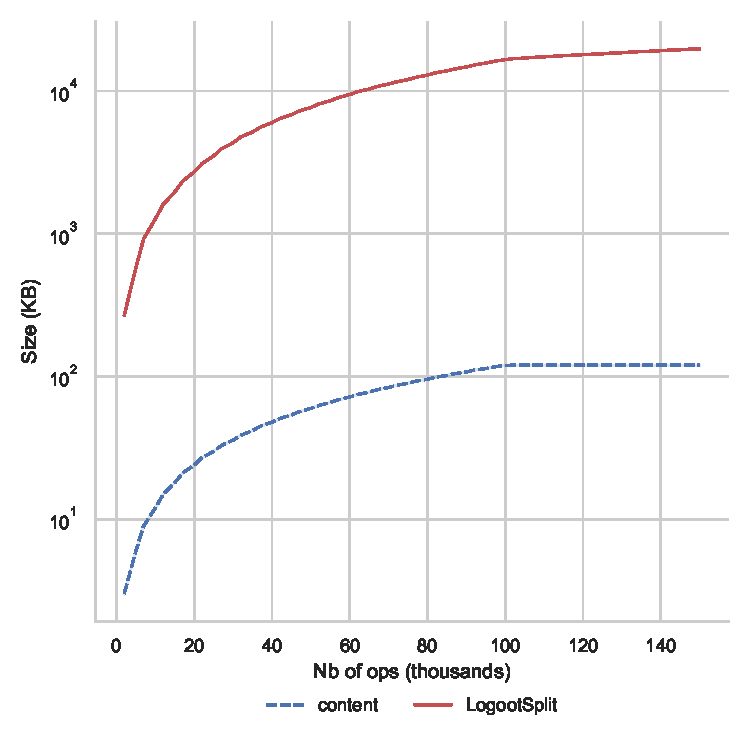
\includegraphics{img/ls-vs-content-snapshot-sizes-7k5.pdf}
  }
  \caption{Taille du contenu comparé à la taille de la séquence LogootSplit}
  \label{fig:size-snapshots-content-vs-ls}
\end{figure}

Sur cette figure, nous représentons l'évolution de la taille en mémoire d'une séquence au fur et à mesure que des modifications sont effectuées sur cette dernière.
Les mesures de la taille de la séquence sont effectuées toutes les 10k modifications.
À partir des résultats obtenus, nous présentons les courbes suivantes :
\begin{enumerate}
  \item La courbe pointillée bleu représente la taille du contenu.
    Ainsi, elle correspond à la taille en mémoire nécessaire pour stocker les éléments en utilisant le type Séquence séquentiel.
  \item La courbe continue rouge représente la taille en mémoire de la séquence LogootSplit complète, \ie la taille de son contenu et de ses métadonnées (identifiants, blocs\dots).
\end{enumerate}

Nous constatons que le contenu représente à terme moins de 1\% de taille de la structure de données.
Les 99\% restants correspondent aux métadonnées utilisées par la séquence répliquée, \ie la taille des identifiants, les blocs composant la séquence LogootSplit, mais aussi la structure de données utilisée en interne pour représenter la séquence de manière efficace.

Nous jugeons donc nécessaire de proposer des mécanismes et techniques afin de mitiger le surcoût des \acp{CRDT} pour le type Séquence et sa croissance.

\mnnote{
  TODO: Serait plus intéressant de proposer des stats sur la taille des ids, le nombre de blocs composant la séquence, le nombre d'éléments par blocs et la proportion de la taille du contenu sur la taille de la structure de données en fonction du nombre d'opérations jouées.
  Pose la question de quand introduire le protocole suivi pour générer les traces.
}


\section{Mitigation du surcoût des séquences répliquées sans conflits}

\begin{itemize}
  \item Plusieurs approches ont été proposées pour réduire croissance des métadonnées dans Sequence \acp{CRDT}
  \item \ac{RGA} (et RGASplit) propose un mécanisme de GC des pierres tombales.
    Nécessite cependant stabilité causale des opérations de suppression.
    S'agit d'une contrainte forte, peu adaptée aux systèmes dynamiques à large échelle.
    \mnnote{TODO: Trouver référence sur la stabilité causale dans systèmes dynamiques}
  \item Core \& Nebula propose un mécanisme de ré-équilibrage de l'arbre pour Treedoc.
    Le ré-équilibrage a pour effet de supprimer des potentielles pierres tombales et de réduire la taille des identifiants.
    Repose sur un algorithme de consensus.
    S'agit de nouveau d'une contrainte forte pour systèmes dynamique à large échelle.
    Pour y pallier, propose de séparer les pairs entre deux ensembles : Core et Nebula.
    Permet de limiter le nombre participant au consensus.
    Un protocole de rattrapage permet aux noeuds de la Nebula de mettre à jour leurs modifications concurrentes à un ré-équilibrage.
  \item LSEQ adopte une autre approche.
    Part du constat que les identifiants dans Logoot croissent de manière linéaire.
    Vise une croissance logarithmique des identifiants.
    Pour cela, propose de nouvelles fonctions d'allocation des identifiants visant à maximiser le nombre d'identifiants insérés avant de devoir augmenter la taille de l'identifiant.
    Propose aussi d'utiliser une base exponentielle pour la valeur \emph{position} des identifiants.
    Atteint ainsi la croissance polylogarithmique des identifiants, sans coordination requise entre les noeuds et mécanisme supplémentaire.
    Solution adaptée aux systèmes distribués à large échelle.
    Conjecture cependant que cette approche se marie mal avec les Sequence \acp{CRDT} utilisant des blocs.
    En effet, ajoute une raison supplémentaire à la croissance des identifiants : l'insertion entre identifiants contigus.
    Force alors la croissance des identifiants.
\end{itemize}

\section{Synthèse}

\begin{itemize}
  \item Systèmes distribués adoptent le modèle de la réplication optimiste pour offrir de meilleures performances, \ie disponibilité et latence, et assurer la résilience du système, \ie accroître la capacité de tolérance aux pannes.
  \item Ce modèle autorise les noeuds à modifier leur copie sans coordination, provoquant ainsi des divergences temporaires.
    Pour résoudre les potentiels conflits et assurer la convergence à terme des copies, systèmes utilisent les \acp{CRDT} en place et lieu des types de données séquentiels.
  \item \acp{CRDT} pour Séquence ont été proposés pour conception d'éditeurs collaboratifs pair-à-pair.
    Deux approches sont utilisées pour concevoir leur mécanismes de résolution de conflits : l'approche basée sur les pierres tombales et l'approche basée sur les identifiants densément ordonnés.
  \item Chacune de ces approches introduit un surcoût croissant, pénalisant leurs performances à terme.
    Plusieurs travaux ont été proposés pour limiter ce surcoût, notamment \cite{letia:hal-01248270, zawirski:hal-01248197} qui présentent un mécanisme de renommage des identifiants pour les \acp{CRDT} pour Séquence basés sur identifiants densément ordonnés.
  \item Mais cette approche requiert un mécanisme de consensus, des renommages concurrents provoquant un nouveau conflit.
    Cette contrainte empêche son utilisation dans les systèmes pair-à-pair ne disposant pas de noeuds suffisamment stables et bien connectés pour exécuter le mécanisme de consensus.
\end{itemize}

\section{Proposition}

\begin{itemize}
  \item Dans ce manuscrit, nous proposons et présentons un nouveau mécanisme de renommage pour \acp{CRDT} pour Séquence, ne nécessitant pas de coordination synchrone entre les noeuds.
  \item Concevons ce mécanisme pour le \ac{CRDT} pour Séquence LogootSplit, mais principe de notre approche est générique.
    Pourrait ainsi l'adapter et proposer un équivalent pour autres \acp{CRDT} pour Séquence, \eg RGASplit.
  \item Présentons et détaillons notre contribution dans le chapitre suivant.
\end{itemize}

% \import{chapters/}{rls}
% \import{chapters/}{mute}

\NumberThisInToc
\chapter{Conclusions et perspectives}
\minitoc
\section{Résumé des contributions}
\section{Perspectives}

% \begin{itemize}
%   \item Définir stratégie pour déclenchement de l'opération \emph{rename}
%   \item Proposer nouvelles relations \emph{priority} \lepoch
%   \item Utiliser combinaison de CRDT et OT pour concevoir structures de données répliquées complexes (move dans Sequence, DFS...)
% \end{itemize}

\subsection{Définition de relations de priorité pour minimiser les traitements}
\subsection{Redéfinition de la sémantique du renommage en déplacement d'éléments}
\subsection{Définition de types de données répliquées sans conflits plus complexes}

\subsection{Étude comparative des différentes familles de CRDTs}

\begin{itemize}
  \item La spécification récente des Delta-based CRDTs .
    Ce nouveau type de CRDTs se base sur celui des State-based CRDTs.
    Partage donc les mêmes pré-requis :
    \begin{itemize}
      \item États du type de données répliqué forment un sup-demi-treillis
      \item Modifications locales entraînent une inflation de l'état
      \item Possède une fonction de \texttt{merge}, permettant de fusionner deux états S et S', et qui
      \begin{itemize}
        \item Est associative, commutative et idempotente
        \item Retourne S", la \ac{LUB} de S et S' (\ie $\nexists S''' \cdot merge(S, S') < S''' < S''$)
      \end{itemize}
    \end{itemize}
    Et bénéficie de son principal avantage : synchronisation possible entre deux pairs en fusionnant leur états, peu importe le nombre de modifications les séparant.
  \item Spécificité des Delta-based CRDTs est de proposer une synchronisation par différence d'états.
    Plutôt que de diffuser l'entièreté de l'état pour permettre aux autres pairs de se mettre à jour, idée est de seulement transmettre la partie de l'état ayant été mise à jour.
    Correspond à un élément irréductible du sup-demi-treillis.
    Permet ainsi de mettre en place une synchronisation en temps réel de manière efficace.
    Et d'utiliser la synchronisation par fusion d'états complets pour compenser les défaillances du réseau
  \item Ainsi, ce nouveau type de CRDTs semble allier le meilleur des deux mondes :
    \begin{itemize}
      \item Absence de contrainte sur le réseau autre que la livraison à terme
      \item Propagation possible en temps réel des modifications
    \end{itemize}
    Semble donc être une solution universelle :
    \begin{itemize}
      \item Utilisable peu importe la fiabilité réseau à disposition
      \item Empreinte réseau du même ordre de grandeur qu'un Op-based CRDT
      \item Utilisable peu importe la fréquence de synchronisation désirée
    \end{itemize}
    Pose la question de l'intérêt des autres types de CRDTs.
  \item Delta-based CRDT est un State-based CRDT dont on a identifié les éléments irréductibles et qui utilise ces derniers pour la propagation des modifications plutôt que l'état complet.
    Famille des State-based CRDTs semble donc rendue obsolète par celle des Delta-based CRDTs.
    À confirmer.
  \item Les Op-based CRDTs proposent une spécification différente du type répliqué de leur équivalent Delta-based, généralement plus simple.
    À première vue, famille des Op-based CRDTs semble donc avoir la simplicité comme avantage par rapport à celle des Delta-based CRDTs.
    S'agit d'un paramètre difficilement mesurable et auquel on peut objecter si on considère qu'un Op-based CRDT s'accompagne d'une couche livraison de messages, qui cache sa part de complexité.
    Intéressant d'étudier si la spécification différente des Op-based CRDTs présente d'autres avantages par rapport aux Delta-based CRDTs : performances (temps d'intégration des modifications, délai de convergence...), fonctionnalités spécifiques (composition, undo...)
  \item But serait de fournir des guidelines sur la famille de CRDT à adopter en fonction du cas d'utilisation.
\end{itemize}

\subsection{Définition d'opérations supplémentaires pour fonctionnalités liées à l'édition collaborative}

\begin{itemize}
  \item Commentaires
  \item Suggestions
\end{itemize}

\subsection{Conduction d'expériences utilisateurs d'édition collaborative}

\begin{itemize}
  \item Absence d'un dataset réel et réutilisable sur les sessions d'édition collaborative
  \item Généralement, expériences utilisent données d'articles de Wikipédia \mnnote{TODO: Revoir références, mais me semble que c'est celui utilisé pour Logoot, LogootSplit et RGASplit entre autres}.
    Mais ces données correspondent à une exécution séquentielle, \ie aucune édition concurrente ne peut être réalisée avec le système de résolution de conflits de Wikipédia.
    \mnnote{TODO:
      Me semble que Kleppmann a aussi utilisé et mis à disposition ses traces correspondant à la rédaction d'un de ses articles.
      Mais que cet article n'était rédigé que par lui.
      Peu de chances de présence d'éditions concurrentes.
      À retrouver et vérifier.
    }
  \item Inspiré par expériences de Claudia, pourrait mener des sessions d'édition collaborative sur des outils orchestrés pour produire ce dataset
  \item Devrait rendre ce dataset agnostique de l'approche choisie pour la résolution automatique de conflits
  \item Absence de retours sur les collaborations à grande échelle
  \item Comment on collabore lorsque plusieurs centaines d'utilisateur-rices ?
\end{itemize}

\subsection{Comparaison des mécanismes de synchronisation}

Serait intéressant de comparer à d'autres méthodes de synchronisation : mécanisme d'anti-entropie basé sur un Merkle Tree\cite{2007-dynamo, 2015-approximate-hash-based-set-reconciliation, 2017-anti-entropy-without-merkle-trees}, synchronisation par états (state/delta-based \acp{CRDT}).
Dans le cadre des Delta-based \acp{CRDT}, pourrait évaluer un protocole de diffusion épidémique des deltas comme celui proposé par SWIM\cite{swim2002}.

\subsection{Distance entre versions d'un document}

\begin{itemize}
  \item Est-ce que ça a vraiment du sens d'intégrer automatiquement des modifications ayant été généré sur une version du document distante de l'état actuel du document (voir distance de Hamming, Levenstein, String-to-string correction problem (Tichy et al))
  \item Jusqu'à quelle distance est-ce que la fusion automatique a encore du sens ?
  \mnnote{NOTE: Peut connecter ça à la nécessité de conserver un chemin d'une époque à l'autre : si les opérations émises depuis cette époque ont probablement plus d'intérêt pour l'état actuel, couper l'arbre ?}
\end{itemize}

\subsection{Contrôle d'accès}

\begin{itemize}
  \item Pour le moment, n'importe quel utilisateur ayant l'URL du document peut y accéder dans MUTE
  \item Pour des raisons de confidentialité, peut vouloir contrôler quels utilisateurs ont accès à un document
  \item Nécessite l'implémentation de liste de contrôle d'accès
  \item Mais s'agit d'une tâche complexe dans le cadre d'un système distribué
  \item Peut s'inspirer des travaux réalisés au sein de la communautée \acp{CRDT} \cite{2021-access-control-crdts, 2022-dist-access-control-pa} pour cela
\end{itemize}

\subsection{Détection et éviction de pairs malhonnêtes}

\begin{itemize}
  \item À l'heure actuelle, MUTE suppose qu'ensemble des collaborateurs honnêtes
  \item Vulnérable à plusieurs types d'attaques par des adversaires byzantins, tel que l'équivoque
  \item Ce type d'attaque peut provoquer des divergences durables et faire échouer des collaborations
  \item \textcite{2021-these-vic} propose un mécanisme permettant de maintenir des logs authentifiés dans un système distribué
  \item Les logs authentifiés permettent de mettre en lumière les comportements malveillants des adversaires et de borner le nombre d'actions malveillantes qu'ils peuvent effectuer avant d'être évincé
  \item Implémenter ce mécanisme permettrait de rendre compatible MUTE avec des environnements avec adversaires byzantins
  \item Nécessiterait tout de même de faire évoluer le \ac{CRDT} pour résoudre les équivoques détectés
\end{itemize}

\subsection{Vecteur de version \emph{epoch-based}}

\begin{itemize}
  \item S'agit d'une structure primordiale dans les systèmes distribués, dont pouvons difficilement nous passer.
    Utilisé notamment pour représenter le contexte causal de l'état d'un noeud, nécessaire pour :
    \begin{enumerate}
      \item Déterminer quelles opérations ont été observées (anti-entropie et couche de livraison)
      \item Déterminer quelles opérations ont observé les autres noeuds (stabilité causale)
      \item Préciser les dépendances causales d'un message
    \end{enumerate}
  \item Comme présenté précédemment, nous utilisons plusieurs vecteurs pour représenter des données dans l'application MUTE
  \item Notamment pour le vecteur de version, utilisé pour respecter le modèle de livraison requis par le \ac{CRDT}
  \item Et pour la liste des collaborateurs, utilisé pour offrir des informations nécessaires à la conscience de groupe aux utilisateurs
  \item Ces vecteurs sont maintenus localement par chacun des noeuds et sont échangés de manière périodique
  \item Cependant, la taille de ces vecteurs croit de manière linéaire au nombre de noeuds impliqués dans la collaboration
  \item Les systèmes \ac{P2P} à large échelle sont sujets au \emph{churn}
  \item Dans le cadre d'un tel système, ces structures croissent de manière non-bornée
  \item Ceci pose un problème de performances, notamment d'un point de vue consommation en bande-passante
  \item Cependant, même si on observe un grand nombre de pairs différents dans le cadre d'une collaboration à large échelle
  \item Intuition est qu'une collaboration repose en fait sur un petit noyau de collaborateurs principaux
  \item Et que majorité des collaborateurs se connectent de manière éphèmère
  \item Serait intéressant de pouvoir réduire la taille des vecteurs en oubliant les collaborateurs éphèmères
  \item Dynamo\cite{2007-dynamo} tronque le vecteur de version lorsqu'il dépasse une taille seuil
  \item Conduit alors à une perte d'informations
  \item Pour la liste des collaborateurs, approche peut être adoptée (pas forcément gênant de limiter à 100 la taille de la liste)
  \item Mais pour vecteur de version, conduirait à une relivraison d'opérations déjà observées
  \item Approche donc pas applicable pour cette partie
  \item Autre approche possible est de réutiliser le système d'époque
  \item Idée serait de ACK un vecteur avec un changement d'époque
  \item Et de ne diffuser à partir de là que les différences
  \item Un mécanisme de transformation (une simple soustraction) permettrait d'obtenir le dot dans la nouvelle époque d'une opération concurrente au renommage
  \item Peut facilement mettre en place un mécanisme d'inversion du renommage (une simple addition) pour revenir à une époque précédente
  \item Et ainsi pouvoir circuler librement dans l'arbre des époques et gérer les opérations \emph{rename} concurrentes
  \item Serait intéressant d'étudier si on peut aller plus loin dans le cadre de cette structure de données et notamment rendre commutatives les opérations de renommage concurrentes
\end{itemize}

\subsection{Fusion de versions distantes d'un document collaboratif}

\subsection{Rôles et places des bots dans systèmes collaboratifs}
\begin{itemize}
  \item Stockage du document pour améliorer sa disponibilité
  \item Overleaf en P2P ?
  \item Comment réinsérer des bots dans la collaboration sans en faire des éléments centraux, sans créer des failles de confidentialité, et tout en rendant ces fonctionnalités accessibles ?
\end{itemize}

\Annex{Entrelacement d'insertions concurrentes dans Treedoc}

\label{app:treedoc-interleaving}

\begin{figure}[!ht]

  \centering
  \resizebox{\columnwidth}{!}{
    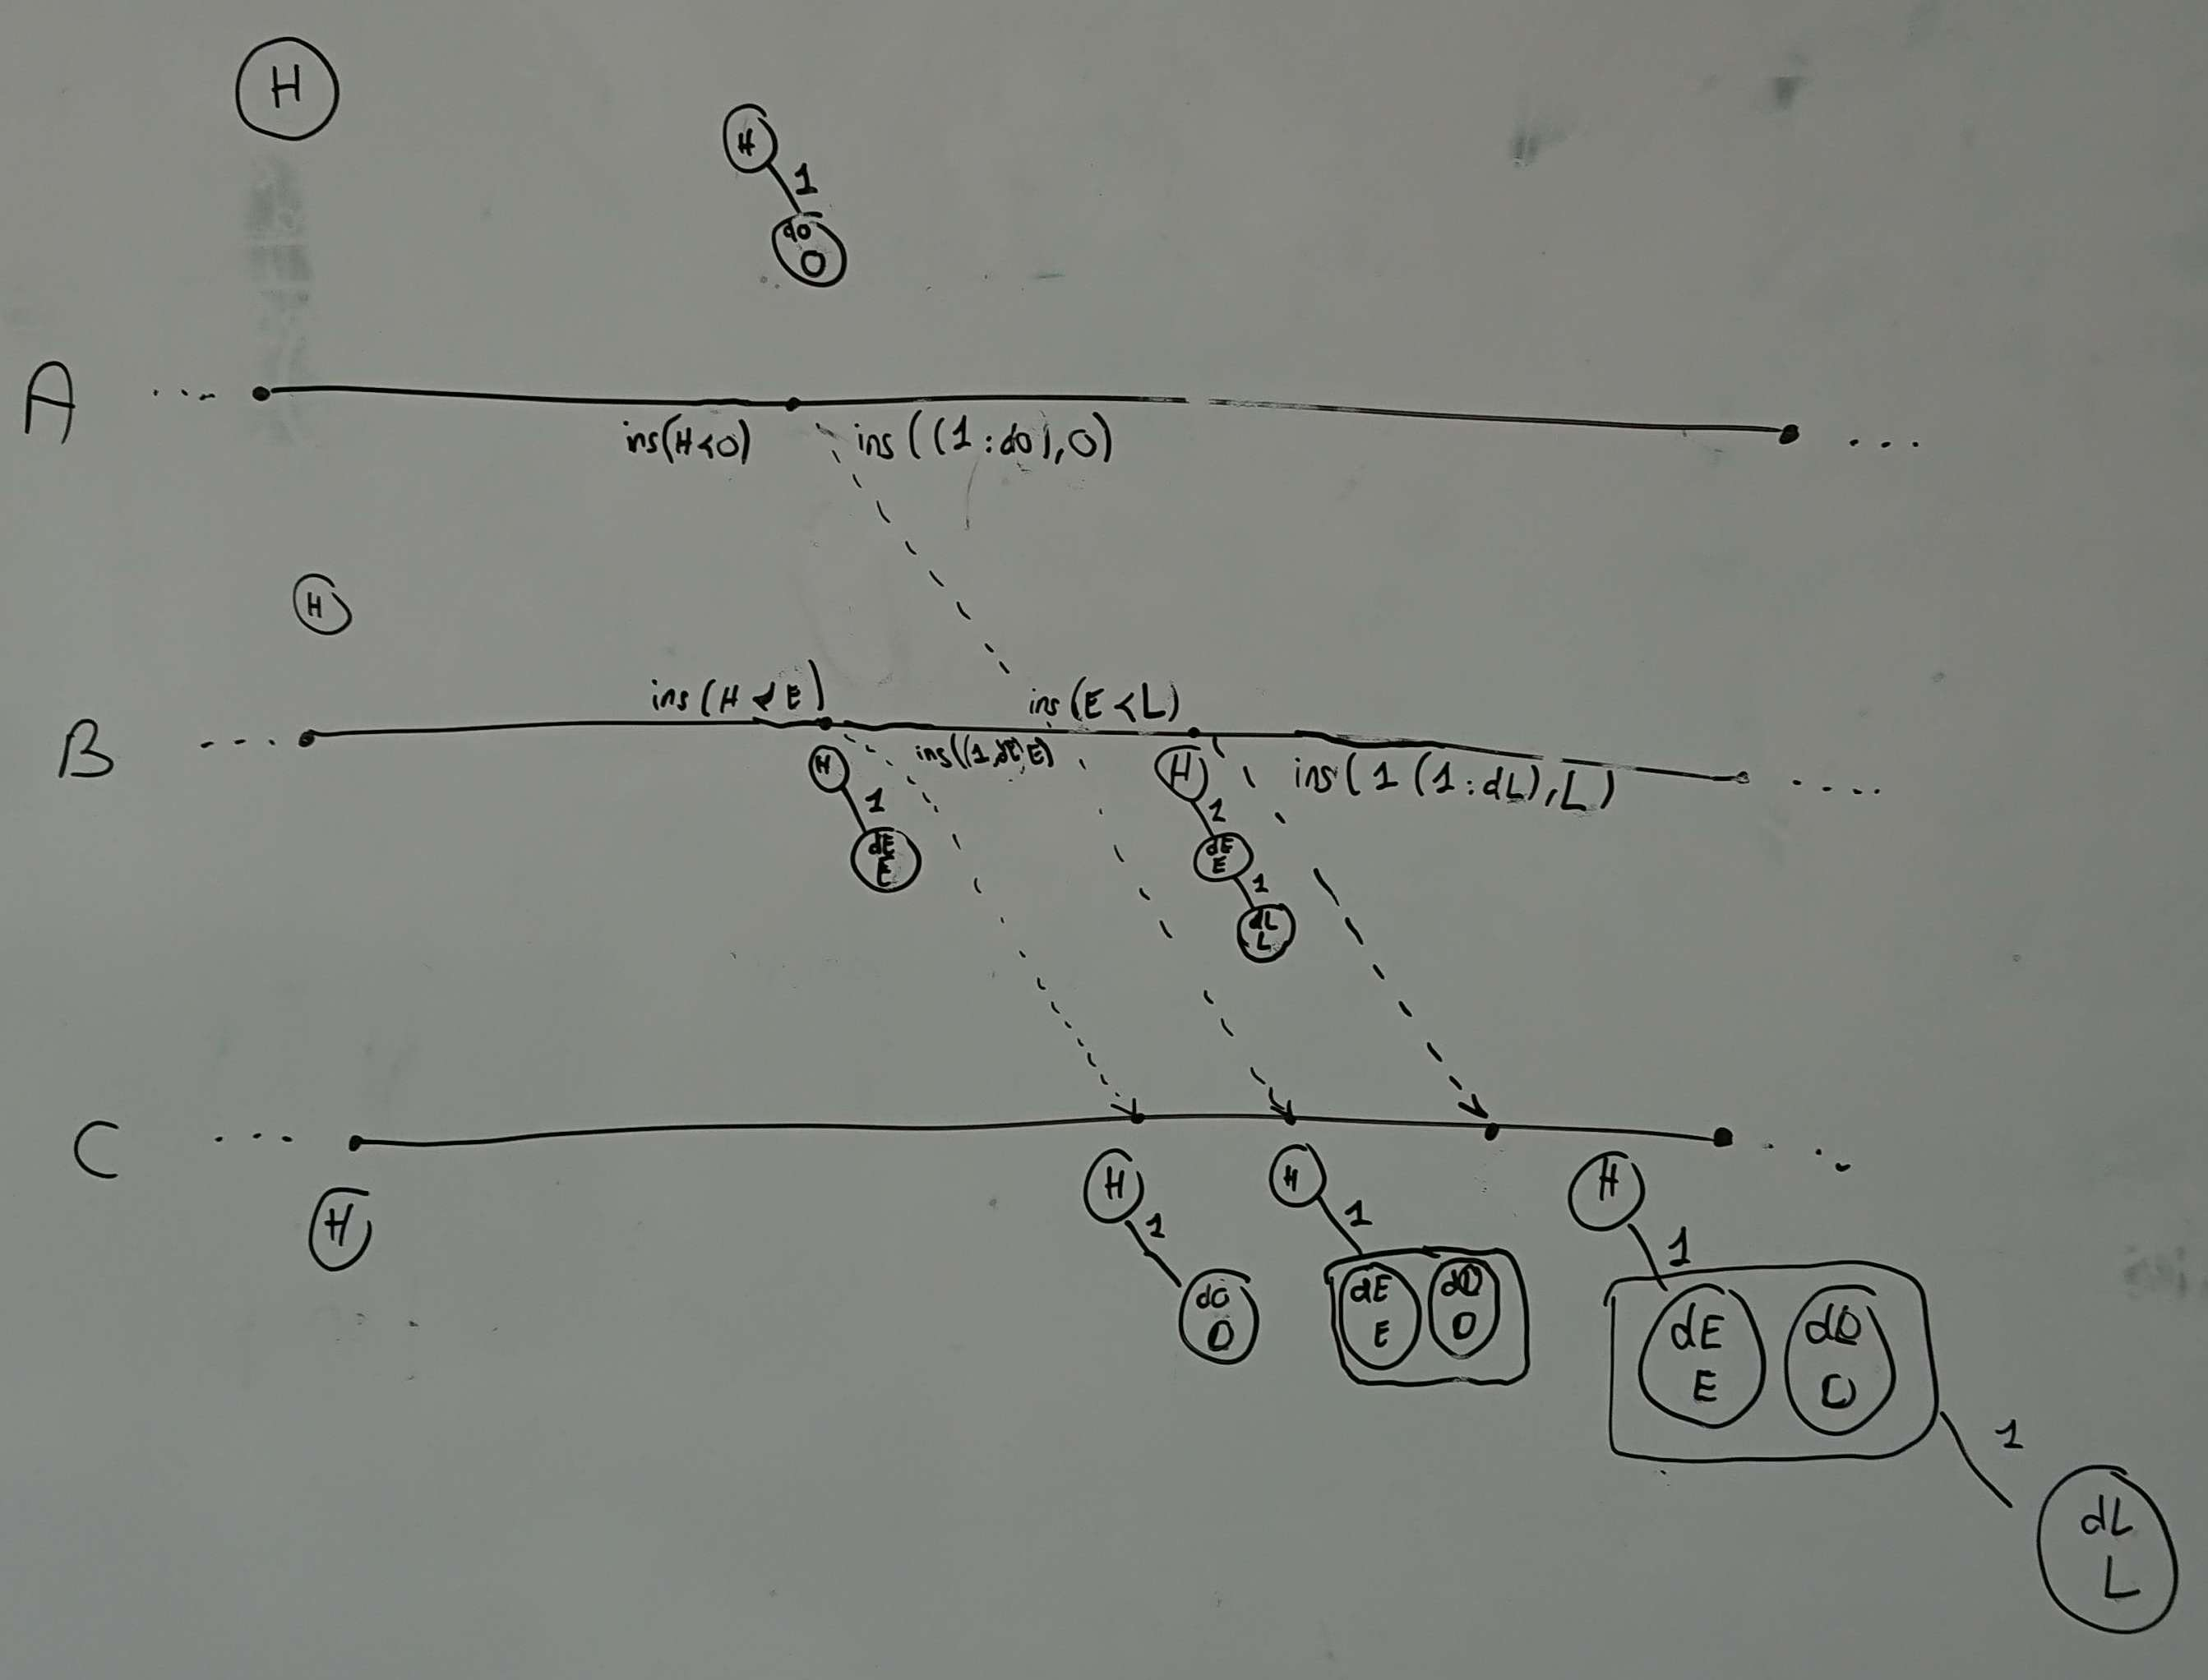
\includegraphics{img/contre-exemple-treedoc}
  }
  \caption{Modifications concurrentes d'une séquence Treedoc résultant en un entrelacement}
\end{figure}

\mnnote{
  TODO: Réaliser au propre contre-exemple.
  Nécessite que $d_E < d_O$, inverser A et B histoire d'éviter toute confusion.
  En soi, C pas nécessaire, à voir si le conserve.
}

\Annex{Algorithmes \textsc{renameId}}

\label{app:rename-id}

\begin{algorithm}[!ht]
  \footnotesize
  \begin{algorithmic}
      \Function{renIdLessThanFirstId}{id, newFirstId}
      \If{id < newFirstId}
          \State \Return id
      \Else
          \State pos $\gets$ position(newFirstId)
          \State nId $\gets$ nodeId(newFirstId)
          \State nSeq $\gets$ nodeSeq(newFirstId)
          \State predNewFirstId $\gets$ \new~Id(pos, nId, nSeq, -1)
          \\
          \State \Return concat(predNewFirstId, id)
          \EndIf
      \EndFunction
      \\
      \Function{renIdGreaterThanLastId}{id, newLastId}
          \If{id < newLastId}
              \State \Return concat(newLastId, id)
          \Else
              \State \Return id
          \EndIf
      \EndFunction
  \end{algorithmic}
  \caption{Remaining functions to rename an identifier}
  \label{alg:appendix-rename-id}
\end{algorithm}

\Annex{Algorithmes \textsc{revertRenameId}}

\label{app:revert-rename-id}

\begin{algorithm}[!ht]
  \footnotesize
  \begin{algorithmic}
      \Function{revRenIdLessThanNewFirstId}{id, firstId, newFirstId}
          \State predNewFirstId $\gets$ createIdFromBase(newFirstId, -1)
          \If{isPrefix(predNewFirstId, id)}
              \State tail $\gets$ getTail(id, 1)
              \If{tail < firstId}
                  \State \Return tail
              \Else
                  \State \Comment{$id$ has been inserted causally after the \emph{rename} op}
                  \State offset $\gets$ getLastOffset(firstId)
                  \State predFirstId $\gets$ createIdFromBase(firstId, offset)
                  \State \Return concat(predFirstId, MAX\_TUPLE, tail)
              \EndIf
          \Else
              \State \Return id
          \EndIf
      \EndFunction
      \\
      \Function{revRenIdGreaterThanNewLastId}{id, lastId}
          \If{id < lastId}
              \State \Comment{$id$ has been inserted causally after the \emph{rename} op}
              \State \Return concat(lastId, MIN\_TUPLE, id)
          \ElsIf{isPrefix(newLastId, id)}
              \State tail $\gets$ getTail(id, 1)
              \If{tail < lastId}
                  \State \Comment{$id$ has been inserted causally after the \emph{rename} op}
                  \State \Return concat(lastId, MIN\_TUPLE, tail)
              \ElsIf{tail < newLastId}
                  \State \Return tail
              \Else
                  \State \Comment{$id$ has been inserted causally after the \emph{rename} op}
                  \State \Return id
              \EndIf
          \Else
              \State \Return id
          \EndIf
      \EndFunction
  \end{algorithmic}
  \caption{Remaining functions to revert an identifier renaming}
  \label{alg:appendix-revert-rename-id}
\end{algorithm}

%
%%-------------------------------------------------------------------
%%                         Le glossaire
%%-------------------------------------------------------------------
%\BeginGloWith{Voici un glossaire tout-à-fait fictif,
%              introduit par un texte sur toute la largeur
%              des deux colonnes.}
%\twocolumn
%\PrintGlossary

%-------------------------------------------------------------------
%              L'index (toujours sur deux colonnes)
%-------------------------------------------------------------------
\BeginIndWith{Voici un index}
\PrintIndex

\onecolumn

%-------------------------------------------------------------------
%                       La bibliographie
%-------------------------------------------------------------------

% La bibliographie (comme d'habitude)

%\nocite{*}
%\bibliographystyle{named}

\printbibliography

%-------------------------------------------------------------------
%                          Les résumés
%-------------------------------------------------------------------
% (si le résumé apparaît sur une colonne étroite, avec la
% bibliographie à gauche, c'est sans doute parce que vous avez
% oublié de générer les fichiers d'index et de glossaire...)

\NumberAbstractPages
\begin{ThesisAbstract}
  \begin{FrenchAbstract}
    Afin d'assurer leur haute disponibilité, les systèmes distribués à large échelle se doivent de répliquer leurs données tout en minimisant les coordinations nécessaires entre noeuds.
    Pour concevoir de tels systèmes, la littérature et l'industrie adoptent de plus en plus l'utilisation de types de données répliquées sans conflits (CRDTs).
    Les CRDTs sont des types de données qui offrent des comportements similaires aux types existants, tel l'Ensemble ou la Séquence.
    Ils se distinguent cependant des types traditionnels par leur spécification, qui supporte nativement les modifications concurrentes.
    À cette fin, les CRDTs incorporent un mécanisme de résolution de conflits au sein de leur spécification.

    Afin de résoudre les conflits de manière déterministe, les CRDTs associent généralement des identifiants aux éléments stockés au sein de la structure de données.
    Les identifiants doivent respecter un ensemble de contraintes en fonction du CRDT, telles que l'unicité ou l'appartenance à un ordre dense.
    Ces contraintes empêchent de borner la taille des identifiants.
    La taille des identifiants utilisés croît alors continuellement avec le nombre de modifications effectuées, aggravant le surcoût lié à l'utilisation des CRDTs par rapport aux structures de données traditionnelles.
    Le but de cette thèse est de proposer des solutions pour pallier ce problème.

    Nous présentons dans cette thèse deux contributions visant à répondre à ce problème :
    \begin{enumerate*}
      \item Un nouveau CRDT pour Séquence, RenamableLogootSplit, qui intègre un mécanisme de renommage à sa spécification.
      Ce mécanisme de renommage permet aux noeuds du système de réattribuer des identifiants de taille minimale aux éléments de la séquence.
      Cependant, cette première version requiert une coordination entre les noeuds pour effectuer un renommage.
      L'évaluation expérimentale montre que le mécanisme de renommage permet de réinitialiser à chaque renommage le surcoût lié à l'utilisation du CRDT.
      \item Une seconde version de RenamableLogootSplit conçue pour une utilisation dans un système distribué.
      Cette nouvelle version permet aux noeuds de déclencher un renommage sans coordination préalable.
      L'évaluation expérimentale montre que cette nouvelle version présente un surcoût temporaire en cas de renommages concurrents, mais que ce surcoût est à terme.
    \end{enumerate*}
    \KeyWords{CRDTs, édition collaborative en temps réel, cohérence à terme, optimisation mémoire, performance}
  \end{FrenchAbstract}
  \begin{EnglishAbstract}
    \KeyWords{CRDTs, real-time collaborative editing, eventual consistency, memory-wise optimisation, performance}
  \end{EnglishAbstract}
\end{ThesisAbstract}


\end{document}



